\documentclass[a4paper,12pt,openright,notitlepage,twoside]{book}
\raggedbottom % lascia alla fine delle pagine lo spazio invece che adattarle


% pacchetti da caricare
\usepackage[T1]{fontenc} % definisce i caratteri di output
\usepackage[utf8]{inputenc} % definisce i caratteri di input
\usepackage[italian,english]{babel} % definisce la lingua del documento
\usepackage{float}
\usepackage[headheight=15pt]{geometry} % definisce i margini del documento
\geometry{a4paper,top=30mm,bottom=30mm,left=30mm,right=25mm,heightrounded,bindingoffset=3mm}
\usepackage{fancyhdr} % serve per gestire intestazione e piè di pagina
\pagestyle{fancy}
\usepackage{multirow}
\usepackage{setspace} % interlinea
\DeclareMathSymbol{\mh}{\mathord}{operators}{`\-}
\usepackage{emptypage} % serve per fare le pagine vuote
\usepackage[pdftex]{hyperref} % serve per ottenere links e indice cliccabili
\hypersetup{colorlinks=true,allcolors=black}
\usepackage{microtype} % migliora la scrittura del testo
\usepackage{appendix} % serve per personalizzare l'appendice
\usepackage[printonlyused]{acronym} % serve per creare l'elenco degli acronimi
\usepackage{eurosym} % serve per scrivere il singolo dell'euro
\usepackage{siunitx} % serve per mettere le unita` di misura nel SI
\usepackage{mathtools} % serve per fare le formule matematiche (carica anche AMSMATH)
\usepackage{booktabs} % serve per fare le tabelle più belle
\usepackage{multirow} % serve per fare le tabelle con righe complesse
\usepackage{pgfplotstable} % serve per fare tabelle da file con dati tabulati
\usepackage{graphicx} % serve per fare le figure
\usepackage{tikz} % serve per fare i grafici
\usepackage{pgfplots} % serve a fare i grafici anche lui
\pgfplotsset{compat=1.14}
\usepackage{subcaption} % serve per aggiungere la didascalia alle figure composte (carica anche CAPTION)
\captionsetup{font=small,labelsep=period,format=hang}
\usepackage{tocloft} % serve per fare le liste di figure e tabelle più belle
\usepackage{cite} % serve per mettere le citazioni bibliografiche

% and from https://tex.stackexchange.com/questions/319805/how-to-include-bibliography-in-table-of-content:
\usepackage[nottoc,notlot,notlof]{tocbibind}

%\usepackage{eurosym}
%\usepackage{mathabx}
\usepackage{amsmath,amssymb}

% modifiche dei comandi
\renewcommand{\chaptermark}[1]{\markboth{\chaptername\ \thechapter.\ #1}{}} % modifica l'intestazione con il nome/numero del capitolo
\renewcommand{\sectionmark}[1]{\markright{\thesection.\ #1}} % modifica l'intestazione con il nome/numero dela sezione
\renewcommand{\cftfigfont}{Figure } % per aggiungere "Figure " nella lista delle figure
\renewcommand{\cfttabfont}{Table } % per aggiungere "Table " nella lista delle tabelle



% dichiarazioni personalizzate
\DeclarePairedDelimiter{\abs}{\lvert}{\rvert} % per fare il valore assoluto
\DeclarePairedDelimiter{\norma}{\lVert}{\rVert} % per fare la norma



\begin{document}

%\frontmatter % serve per mettere i numeri romani come numeri di pagina 
\thispagestyle{empty} % serve per rimuovere tutte le impostazioni delle pagine dalla prima pagina

% FRONTESPIZIO
\begin{center}
% Intestazione
\Large{\textbf{Politecnico di Milano}} \\
\vspace{-2mm}
\rule{\textwidth}{0.4pt}
\normalsize{SCHOOL OF INDUSTRIAL AND INFORMATION ENGINEERING} \\
\normalsize{Master of Science in Computer Science and Engineering} \\
\vspace{20mm}
% Logo Politecnico
\begin{figure}[h!]
\centering

\includegraphics[height=0.20\textheight]{images/logo_poli_bianco}
\end{figure}
\vspace{12mm}
% Titolo Tesi
\huge{\textbf{Brain Magnetic Resonance Imaging Generation using Generative Adversarial Networks}} \\
\vspace{22mm}
\end{center}

% Relatore/Correlatore
\begin{flushleft}
\normalsize{Supervisor} \\
\small{\textbf{Daniele LOIACONO}} \\
\vspace{5mm}
\normalsize{Co-Supervisor} \\
\small{\textbf{Edoardo GIACOMELLO}} \\
\end{flushleft}
\vspace{10mm}

% Autore
\begin{flushright}
\normalsize{Candidate} \\
\small{\textbf{Emanuel ALOGNA -- 893592}} \\
\end{flushright}
\vspace{15mm}

% Piè Di Pagina
\begin{center}
\rule{\textwidth}{0.4pt}
\small{\textbf{Academic Year 2018 -- 2019}}
\end{center}


% modifica intestazione e piè di pagina del corpo del documento
\fancyhead{} % cancella tutti i campi dell'intestazione
\fancyfoot{} % cancella tutti i campi del piè di pagina
\fancyhead[LE,RO]{\leftmark}
\fancyfoot[LE,RO]{\thepage}
\renewcommand{\headrulewidth}{0.4pt}
\renewcommand{\footrulewidth}{0pt}


% carico le varie parti della tesi

\chapter*{ }
\label{cha:dedication}
%\markboth{Abstract}{}
%\thispagestyle{empty}
\begin{flushright}
\textit{To the ones that never stop believing in themselves.}

\vspace{3mm}
\textit{To the fools who always dream.}

% To the ones that never stop to believe in themselves. To the fools who dream, always.
\end{flushright}



%\mainmatter
\chapter*{Ringraziamenti}
\label{cha:acknowledgements}
\markboth{Ringraziamenti}{}
%\addcontentsline{toc}{chapter}{Acknowledgements}

\textit{Prima di tutto vorrei ringraziare il Prof. Daniele Loiacono, mio relatore e guida in questo percorso non privo di difficoltà, e il Dott. Edoardo Giacomello per la loro grande disponibilità durante questi mesi di lavoro ma anche per la pazienza mostrata, il continuo supporto, gli spunti fondamentali e i confronti costruttivi che mi hanno permesso di realizzare questa tesi. Grazie per avermi stimolato e permesso di appassionarmi ancora di più a questa materia.}

\vspace{5mm}
\noindent\textit{Grazie a mia mamma e mio papà, che non hanno mai smesso di incoraggiarmi e mi hanno supportato (e sopportato) in ogni modo possibile durante questi anni, permettendomi di concentrarmi sullo studio a tempo pieno e dandomi la possibilità di vivere una bellissima esperienza all'estero. Tutto questo, senza di loro, non sarebbe stato possibile.}

\vspace{5mm}
\noindent \textit{Un ringraziamento speciale ai miei fratelli che mi spingono a mettermi sempre in gioco: a Dani, la persona con la quale ho sempre potuto parlare di qualsiasi cosa, e a Mirko che, nonostante la distanza, non ha mai fatto mancare i suoi preziosi consigli. Grazie a Simona, che ormai è come una sorella, e grazie a nonna Uccia, che aspettava più di chiunque altro questo momento.}

\vspace{5mm}
\noindent \textit{Ringrazio Liuch, collega nonchè uno dei miei migliori amici, con cui ho avuto la fortuna di condividere questi cinque anni universitari, un progetto dopo l'altro, esame dopo esame. Finalmente siamo riusciti a tagliare questo traguardo. }


\noindent \textit{Un grazie speciale anche a Ippo, Rich, Erik e Barte per esserci sempre stati, anche nei momenti difficili. Amici di una vita, con cui spero di condividere ancora tanti momenti come questo.}

\vspace{5mm}
\noindent \textit{Desidero inoltre ringraziare Lollo e Lello, compagni di studio in biblioteca fino a tarda notte, e grazie a Gio, per le domeniche passate in aula studio sin dalla mattina e per le sciate in montagna in uno dei momenti di maggiore stress di questi mesi. Grazie infine a Salva, Dave, Mutto e Fabio che, tra calcetti e pause in biblioteca, hanno reso più leggeri gli ultimi anni di questo viaggio.}
%\setcounter{page}{1}
\cleardoublepage

% Indice 
\phantomsection
\addcontentsline{toc}{chapter}{\contentsname}
\tableofcontents
\cleardoublepage

% Lista delle Figure
\phantomsection
\addcontentsline{toc}{chapter}{\listfigurename}
\listoffigures
\cleardoublepage


% Lista delle Tabelle
\phantomsection
\addcontentsline{toc}{chapter}{\listtablename}
\listoftables
\cleardoublepage



\chapter*{Abstract}
\label{cha:abstract}
\markboth{Abstract}{}
\addcontentsline{toc}{chapter}{Abstract}
\onehalfspace
\ac{MRI} is nowadays one of the most common medical imaging techniques, due to the non-invasive nature of this type of scan that can acquire many modalities (or sequences), each one with a different image appearance and unique insights about a particular disease. However, it is not always possible to obtain all the sequences required, due to many issues such as prohibitive scan times or allergies to contrast agents. To overcome this problem and thanks to the recent improvements in Deep Learning, in the last few years researchers have been studying the applicability of \ac{GAN} to synthesize the missing modalities. Our work proposes a detailed study that aims to demonstrate the power of GANs in generating realistic \ac{MRI} scans of brain tumors through the implementation of different models.  We trained in particular two kind of networks which differ from the number of sequences received in input, using a dataset composed by 274 different volumes from subjects with brain tumor, and, among a set of different evaluation metrics implemented to test our results, we validated the quality of the predicted images using also a segmentation model.
In addition, we analysed the \ac{GAN}s trained by performing some experiments to understand how the information passes through the generator network. Our results show that the synthesized sequences are highly accurate, realistic and in some cases indistinguishable from true brain slices of the dataset, highlighting the advantage of multi-modal models that, compared to the unimodal ones, can exploit the correlation between available sequences. Moreover, they demonstrate the effectiveness of skip connections and their crucial role in the generative process by showing the significant degradation in the performances, analysed in both a qualitative and quantitative way, when these channels are turned off or perturbed.
\chapter*{Estratto in lingua Italiana}
\label{cha:estratto}
\markboth{Estratto}{}
\addcontentsline{toc}{chapter}{Estratto in lingua Italiana}

L'imaging a risonanza magnetica (\ac{MRI}) è oggi una delle più comuni tecniche di generazione di immagini mediche, per via della natura non invasiva di questo tipo di scansione che permette di acquisire varie modalità (o sequenze) della parte del corpo scansionata, ognuna diversa dall'altra per livello di risoluzione e contrasto utilizzato.  Tuttavia, non è sempre possibile ottenere tutte le sequenze richieste, a causa di molteplici problemi, tra cui i tempi di scansione proibitivi o le allergie dei pazienti agli agenti di contrasto. Per ovviare a questo problema e grazie ai recenti miglioramenti nel campo del Deep Learning, negli ultimi anni i ricercatori hanno studiato l'applicabilità delle Reti Antagoniste Generative (\ac{GAN}) alla generazione delle modalità mancanti. Il nostro lavoro propone uno studio dettagliato che mira a dimostrare l'abilità delle GAN nel generare scansioni MRI realistiche di tumori cerebrali attraverso l'implementazione di diversi modelli. Abbiamo allenato in particolare due tipi di reti che differiscono per il numero di sequenze ricevute in input, utilizzando un dataset composto da 274 diversi volumi appartenenti a pazienti con tumori cerebrali e, tra una serie di diverse metriche implementate per valutare i nostri risultati, abbiamo validato la qualità dell'immagine generata dalla rete usando anche un modello di segmentazione.
Inoltre, abbiamo analizzato le \ac{GAN} addestrate, eseguendo alcuni esperimenti per capire come il contenuto informativo ricevuto in input passi attraverso il generatore, ovvero una delle due reti neurali che compongono una GAN. I nostri risultati dimostrano che le sequenze sintetizzate sono altamente accurate, realistiche e in alcuni casi indistinguibili dalle immagini provenienti dal dataset, evidenziando il vantaggio dei modelli multi-input che, rispetto a quelli single-input, possono sfruttare la correlazione presente tra le sequenze che sono disponibili. Inoltre, dimostrano l'efficacia delle skip connections e il loro ruolo fondamentale nel processo generativo mostrando come, spegnendo o perturbando i canali, le prestazioni della rete subiscano un calo significativo.



%\chapter*{Extended Abstract}
\label{cha:extended_abstract}
\markboth{Extended Abstract}{}
\addcontentsline{toc}{chapter}{Extended Abstract}
\onehalfspace
Lorem ipsum dolor sit amet, consectetur adipisci elit, quis nostrum exercitationem ullam corporis suscipit laboriosam, nisi ut aliquid ex ea commodi consequatur.
\cleardoublepage


% modifica intestazione indice
\fancyhead[LE,RO]{\nouppercase{\leftmark}} % cancella il tutto maiuscolo


\fancyhead[LE]{\leftmark}
\fancyhead[RO]{\rightmark}
\fancyfoot[LE,RO]{\thepage}

%\mainmatter % serve per mettere i numeri arabi come numeri di pagina

\onehalfspace
% Capitoli Tesi
\chapter{Introduction}
\label{cha:first_chapter}
Medical imaging is crucial for clinical analysis and medical intervention since it gives important insights about some diseases whose structures might be hidden by the skin or by the bones. 
One of the most common techniques used nowadays is the Magnetic Resonance Imaging (~\ac{MRI}), ubiquitous in hospitals and medical centers, first because of its non-invasive nature, since, differently from other imaging technologies, doesn't make use of X-ray radiography and secondly because of the recent improvements in the software and hardware instrumentation used.
In this type of imaging, various sequences (or modalities) can be acquired and each sequence can give useful and different insights about a particular problem of the patient. For example the $T_{1}$-weighted sequence can distinguish between gray and white matter tissues while $T_{2}$-weighted is more indicated to highlight fluid from cortical issue.

\vspace{5mm} %5mm vertical space
The problem about MRI is that sometimes there isn't the possibility to acquire all the sequences that would be required in order to diagnose a disease and this is due to different reasons: sometimes there isn't enough time to collect all the needed sequences, sometimes it's too expensive to acquire all of them. Furthermore, missing sequences might occur because of allergies in the patient that don't allow to obtain modalities where an exogenous contrast agent, a substance useful to increase the contrast between structures or fluids within the target area, is used to make the image clearer. It can also happen that, for a given patient, some scans might be unusable due to the presence of errors, corruptions or machine settings not defined in the proper way\cite{migan}.

\vspace{5mm} %5mm vertical space
It would be useful, then, to find a way to generate a prediction of the missing sequences by using the modalities already acquired for a given patient.
These generated predictions then could be used either as direct aid to the doctor that has to make a diagnosis for a patient that maybe can't have injected into his body any kind of contrast agent, or could be used as one of the input pieces of a bigger pipeline.

\vspace{5mm} %5mm vertical space
Thanks to the recent improvements in Machine Learning, but more in particular in the~\ac{DL} field, the generation of missing modalities has become an objective feasible to reach, both in terms of efficiency of the obtained result and in terms of time spent in order to reach something meaningful.

\vspace{5mm} %5mm vertical space
In the last few years interest toward Machine Learning and Deep Learning has grown exponentially: just to give an idea to the incredible spread that is having this~\ac{AI} research area, in the 2016 and 2017 over 400 contributions related to Deep Learning applied to Medical Image Analysis were published\cite{Yi_2019}.
%In the \cite{review}
It has been shown that~\ac{DL} has been able to reach very competitive results in many medical task: classification, detection, segmentation, registration of different areas and structures within the human body.
Many progresses have been done and further are yet to come in order to reach results as accurate and precise as possible in crucial applications such as cancer cell classification, lesion detection, organ segmentation and image enhancement\cite{Litjens_2017}.

\vspace{5mm} %5mm vertical space
The most successful~\ac{DL} architecture in medical image analysis is the \ac{CNN}: a neural network with multiple hidden layers between the input and the output layers. The initial problem with this type of architecture was that researchers weren't able to train these deep neural networks in an efficient way.
A breakthrough was the work described in\cite{dl} that represents a huge contribution to the field since the proposed CNN, called AlexNet, won the ImageNet competition in 2012 by a large margin. The peculiarity of AlexNet was that its competitive results and high performances were obtained in relative short time, due to the fact that the designer of this network made the training feasible by the utilization of a~\ac{GPU}.

\vspace{5mm} %5mm vertical space
Another important breakthrough in the field was represented by the introduction of Generative Adversarial Networks, a class of machine learning systems invented by Ian J. GoodFellow in 2014\cite{gan} that we used in this work to solve the problem of missing modalities.

\section{Scope}
\label{sec:scope}
In this work we study the applicability of Generative Adversarial Networks to the domain of medical imaging, by focusing on the generation of brain MRI sequences in order to overcome the problem of missing or unusable modalities and so to avoid repeating the exams multiple times.
In particular, we propose a detailed study on the predictive power of three different \ac{GAN} implemented: the first one is a unimodal model proposed by Isola et al. and called pix2pix \cite{pix2pix}, while the other two networks are MI-pix2pix, a multi-input version of pix2pix, and MI-GAN, a modified version of the MM-GAN proposed by Sharma et al. in \cite{migan}, adapted to the multi-input single-output scenario. 

We evaluate, then, the results obtained from the trained networks by assessing the performances in both a qualitative way, so with human perception, and a quantitative way, through different metrics implemented to test the generated quality of the tumor area, that needs to be synthesized with high accuracy, as well as the overall quality of the whole image. 

Moreover, for studying the capabilities of the network and how skip connections affect the generative process, we show how much the performances can deteriorate by switching off or perturbing the channels in the generator network.  

The two main contributions of this work can be summarized as follows:

\begin{itemize}
\item We define and compare two multi-modal \ac{GAN}s, MI-pix2pix and MI-GAN, that receive the same number of inputs but have different architectures and use different loss functions.
\item We present a systematic analysis of skip connections that extends the analysis of the generator architecture in \cite{pix2pix}.
\end{itemize}


\vspace{5mm} %5mm vertical space


\section{Thesis Structure}
\label{sec:third_section}
In Chapter \ref{cha:2nd_chapter} we present the related work and the theoretical background needed to make more understandable the work discussed in the following chapters. Chapter \ref{cha:3rd_chapter} describes in detail the dataset used and how it has been preprocessed in order to make it work with our models.
In Chapter \ref{cha:4th_chapter} we present to the reader the neural network architecture implemented, along with the training algorithm and the metrics that we decided to use in order to evaluate, quantitatively, the results obtained, that are presented in Chapter \ref{cha:5th_chapter}. In Chapter \ref{cha:6th_chapter} further experiments on our trained models are described. Finally, Chapter \ref{cha:7th_chapter} contains our general considerations about this work, a description of the open problems related to the topic and a discussion on possible applications and future develops.
\chapter{State of the Art}
\label{cha:2nd_chapter}
In this chapter we first present the related work on the Generative Adversarial Networks in the literature (\ref{sec:related_work}) and then, in Section \ref{sec:theoretical_background}, we introduce the theoretical aspects our work is based upon, while giving the reader an overview of the tools and techniques we applied in our models, in order to better understand the setting in which our work takes place.

\section{Related Work}
\label{sec:related_work}
\ac{GAN}s have been used in many data domains, but the images one is where this type of neural network obtained the most significant results so far. In \cite{gan} this architecture has been tested for the first time on a range of image datasets including MNIST\cite{lecun}, the Toronto Face Database\cite{tfd} and CIFAR-10\cite{cifar}. Isola et al. applied \ac{GAN}s to the image-to-image translation task and, in order to explore the generality of their work\cite{pix2pix}, experimented with a variety of settings and datasets such as generating the night version of an image whose daily version was given as input to the network or synthesizing the picture of a building by only observing its relative architecture label as input after a training performed on CMP Facades 
(Figure~\ref{fig:first_figure}).
\begin{figure}[htbp!]
\centering
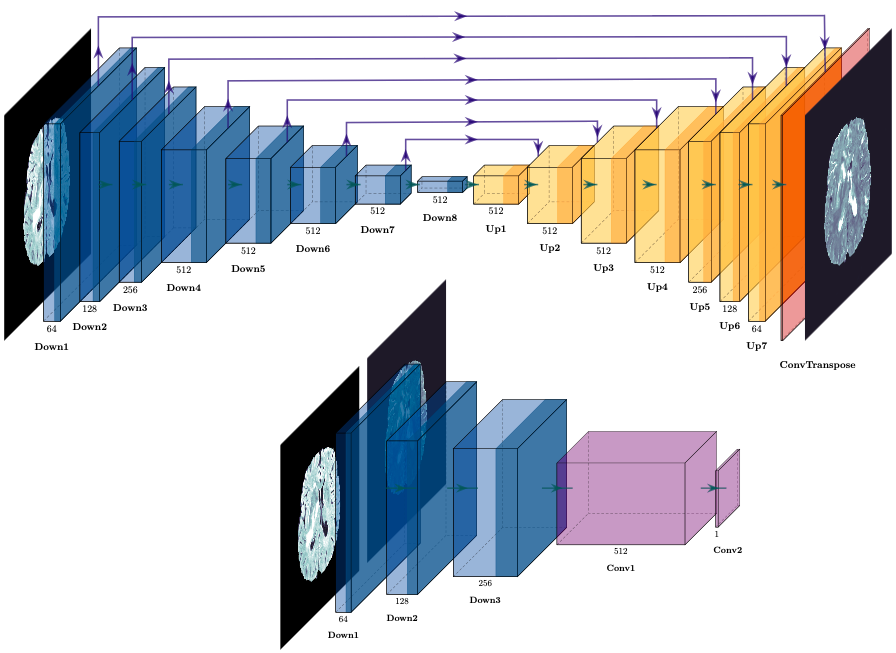
\includegraphics[height=0.235\textheight]{images/pix2pix}
\caption[Pix2Pix example from Isola et al.]{Examples of image-to-image translation from the work of Isola et al. \cite{pix2pix}}
\label{fig:first_figure}
\end{figure}
\subsection{GANs in Medical Imaging}
\label{subsec:gans_medical_imaging}
Countless studies about medical image synthesis were approached using \ac{GAN}s. In particular, cross modality image synthesis (so the conversion of the input image of one modality to the output of another modality) is the most important application of this architecture: in 2018, was even published a review\cite{Yi_2019} about all the work and progresses that have been done in the field of medical imaging through the application of~\ac{GAN}s. The authors described the magnetic resonance as the most common imaging modality explored in the literature related to this generative approach invented by Goodfellow and this is probably due to the fact that~\ac{GAN}s, through the cross modality synthesis, can reduce the excessive amount of time requested from~\ac{MR} acquisition.

\vspace{5mm} %5mm vertical space
Many different approaches and datasets have been used in the literature in order to overcome the problem of missing modalities. Orbes-Arteaga et al., in \cite{flair&t1}, since most of the datasets contain only $T_1$ or $T_1$/$T_2$/PD scans due to logistical reasons, implemented a~\ac{GAN} that generates $T_{2flair}$ of the brain using $T_1$ modality. 
In \cite{lapgan}, Camileri et al. developed a variant of the original GAN, called Laplacian pyramid framework (LAPGAN) that synthesizes images in a coarse-to-fine way. This method, as the name suggests, is based on Laplacian pyramid and allows to generate initially an image with low resolution and then, incrementally, add details to it. Another approach to generate missing modalities was proposed in \cite{double_scenario} where they presented two possible scenarios, based on the given dataset: they use a model called pGAN (that incorporates a pixel-wise loss into the objective function) when the multi-contrast images are spatially registered while they adopt a cycleGAN\cite{cycle_gan}  in the more realistic scenario in which pixels are not aligned between contrasts. A cycleGAN is a~\ac{GAN} variant characterized by the fact that has two generators, two discriminators and uses a cycle consistency loss with a collection of training images from the source and target domain that don't need to be related in any way.

Most of the papers about Generative Adversarial Networks, and also this work, though, are based on a training performed using paired examples, with input image and target image perfectly aligned. 

\vspace{5mm} %5mm vertical space
It is worth to cite also the work done by Anmol Sharma and Ghassan Hamarneh that were, to the best of their knowledge\cite{migan}, the first to propose a many to many generative model, capable of synthesize multiple missing sequences given a combination of various input sequences. Furthermore, they were the first to apply the concept of curriculum learning, based on the variation of the difficulty of the examples that are shown during the network training.

\vspace{5mm} %5mm vertical space
MRI isn't the only imaging technique where~\ac{GAN} has been applied to: in literature is possible to find various publications of generative models that use~\ac{PET},~\ac{CT} or~\ac{MRA} images. 
Olut et al., in 2018, demonstrated that~\ac{GAN} works efficiently even when the source imaging technique is different from the target one: they were the first ones to synthesize~\ac{MRA} brain images from $T_1$ and $T_2$ MRI modalities\cite{mra&mri}. Ben-Cohen et al. published in the same year an article\cite{ct&pet} explaining how to generate~\ac{PET} images using~\ac{CT} scans through a fully connected neural network, whose output is improved and refined by a~\ac{cGAN}\cite{cgan}.


\vspace{5mm} %5mm vertical space
The work related to the generation of medical image is huge and new papers about the topic are being published every week. Many approaches have been already tested and many datasets have been used but there are still lots of challenges that need to be solved in order to be able to be employed in medical imaging\cite{Yi_2019} and since there is still room for improvements in the application of generative models in medical imaging, we present in this work a complete study on different architectures of~\ac{GAN} used to generate missing modalities of brain scans, followed by an analysis of the information that passes through the inner channels and through the skip connections of the generator networks.


\section{Theoretical Background}
\label{sec:theoretical_background}
The architecture of the main model used in our work, the Generative Adversarial Network, is based on the Convolutional Neural Network: a deep neural network with many hidden layers that nowadays is proved successful in many application going from Image Recognition to Video Analysis, passing through Natural Language Processing, Anomaly detection, Drug Discovery, etc.

\subsection{Convolutional Neural Network}
\label{sec:convolutional_neural_network}
The 1980, period in which David H. Hubel and Torsten Wiesel gave crucial insights about the structure of the visual cortex (the researchers are winners of the 1981 Nobel Price in Physiology or Medicine for their work), is the starting point from which \textit{convolutional neural networks} started to gradually evolve into what is today the architecture most used in~\ac{DL}.

\vspace{5mm} %5mm vertical space
The milestone is represented by the work of Yann LeCun that in 1998 developed a model, LeNet-5, to identify handwritten digits for zip code recognition in the postal service\cite{lecun}.
This model was composed by traditional building blocks such as fully connected layers and sigmoid activation functions but also by convolutional layers and pooling layers, introduced for the first time.

The most important building block is the convolutional layer, based on the mathematical operation from which~\ac{CNN} take its name. This layer allows to extract features by convolving the input with a certain number of filters, producing a stack of feature maps, one per each filter that was convolved with the input image.
Each filter basically tries to capture, in the first layers of the network, low-details of the image by producing this feature map that highlights which are the areas on the input that were activated by the filter the most.
In the the next hidden layers this small low-level features are assembled into higher-level features and this hierarchical structure is one of the reason why~\ac{CNN}s work so well and are so widely used\cite{lecun}.

\subsection{Generative Adversarial Network}
\label{subsec:gan}
Generative Adversarial Network was proposed in 2014 by Ian J. GoodFellow\cite{gan} and represents a new framework for estimating generative models in an adversarial setting. The system is composed by two neural networks: a discriminator D, typically a~\ac{CNN}, and a generator G that are trained simultaneously. 

\begin{figure}[H]
\centering
\includegraphics[height=0.27\textheight]{images/GANs.pdf}
\caption[Generative Adversarial Network Framework]{Generative Adversarial Network Framework \cite{GAN_image}.}
\label{fig:GANs}
\end{figure}
In particular, G is trained to learn the probability distribution of the data given as input and to generate synthesized data that exhibits similar characteristics to the authentic data while the discriminative model estimates the probability that a sample came from the training data rather than G.

\vspace{5mm} %5mm vertical space
This adversarial setting is usually explained through the example of the counterfeiter (generator) that tries to produce and use fake money without being caught from the police (discriminator) that, on the other hand, tries to detect the counterfeiter fake currency. The process continues until the counterfeiter becomes able to trick the police with success. \ac{GAN}s work in the same way, with the two networks that compete with each other in a game (corresponding to what is called minimax two-player game in Game Theory \cite[p.~276]{optimization}): the discriminator tries to distinguish true images, belonging to the input dataset, from fake images produced by the generator, whose objective is instead to learn to generate the most realistic data possible to be able to fool D.

Equation~\ref{eq:first_equation} shows the losses for D and G used in the original architecture\cite{gan}.

\begin{equation} \label{eq:first_equation}
\begin{gathered}
L_D^i \leftarrow \frac{1}{m} \sum_{i=1}^{m} [\log D(x^{(i)}) + \log(1 - D(G(z^{(i)})))] \\
L_G^i \leftarrow \frac{1}{m} \sum_{i=1}^{m} \log(1 - D(G(z^{(i)})))
\end{gathered}
\end{equation}
where $z^i$ is a batch of random noise and $x^i$ is a batch of true \textit{m} data samples.
The two networks are trained alternately using \textit{Backpropagation}, in such a way that the generator can learn to synthesize the images based on the discriminator feedback. 

It's important to highlight that the G never sees real images: it just learns the gradients flowing back through the discriminator. The better the discriminator gets, the more information about real images is contained in these secondhand gradients, so the generator can make significant progress\cite[p.~1301]{hands_on_ml}.
As the training advances, the~\ac{GAN} may end up in a situation that is called \textit{Nash equilibrium}, so a situation in which the generator produces perfectly realistic images while the discriminator is forced to guess (50\% real and 50\% fake). Unfortunately, even training a GAN for a long time, there is no guarantee to reach this equilibrium\cite[p.~1307]{hands_on_ml}. 

\subsection{Deep Convolutional GAN (DCGAN)}
\label{subsec:dcgan}
The problem with the original~\ac{GAN} paper \cite{gan} is that GoodFellow et al. experimented with convolutional layers but only with small images.
In the following months researchers tried to work with deeper neural networks for larger images and, in 2015, Radfrod, Metz and Chintala presented an improved version of the original architecture with some tricks and variations\cite{dcgan}.


The guidelines proposed, that we followed in our work, in order to obtain a stable training even with large images, are: 
\begin{itemize}
  \item Replacement of any pooling layers (downsampling layers that allow to reduce the spatial information of the image) with strided convolutions in the discriminator and with transposed convolutions (similar to the convolution layer but goes in the opposite direction by enlarging the spatial dimensions) in the generator.
  \item Batch normalization\cite{batchnormalization} - a normalization of the input computed across the whole batch - in every layer (with the exception of the generator output layer and the discriminator input layer).
  \item Remove fully connected hidden layers (whose neurons are connected to every node of the previous layer), both in G and D.
  \item ReLu as activation functions\cite{relu} in G for all layers except for the output, which uses tanh (hyperbolic tangent activation function with an output range from -1 to +1). ReLu is a non linear function that maps its input between 0 to infinity.
  \item use of Leaky ReLU: activation function similar to ReLU but with a small slope for negative values that avoid neurons to stop outputting anything other than a 0 value. It is used in D for all layers.
\end{itemize}

\begin{figure}[htbp!]
\centering
\includegraphics[height=0.25\textheight]{images/dcgan}
\caption[Layers from DCGAN, Radford, Metz, and Chintala]{DCGAN generator used in the work of Radford, Metz and Chintala.}
\label{fig:dcgan}
\end{figure}

\subsection{Conditional GAN}
\label{subsec:conditional_gan}
In the \textit{Conclusions and future work} of the original~\ac{GAN} paper\cite{cgan}, GoodFellow et al. suggested that the proposed framework could have been extended by conditioning the input of both G and D.
This extension was realized by Mehdi Mirza and Simon Osindero that developed a Conditional Generative Adversarial Net.
The authors explain that in a unconditioned generative setting there is no possibility to control the modes of the data that is generated, while, by conditioning the input with some extra information \textit{y}, it's possible to direct the data generation process\cite{cgan}.

Such extra input can be any kind of auxiliary information, such as class labels or data coming from other modalities (in our work we conditioned the input with images as extra information), so the prior noise \textit{z} is combined to \textit{y} as input to the generator while the discriminator takes as input data \textit{x} and \textit{y.}


\subsection{Image-to-Image translation with Conditional GAN}
\label{subsec:image-to-image_translation}
After the publication, in 2015, of \textit{Conditional Adversarial Nets}\cite{cgan}, many researchers started to apply this kind of architecture to the \textit{Image-to-Image translation}, the task of translating one possible representation of a scene into another one,  using images as auxiliary information to control the data generation. An important contribute was given by Phillip Isola et al. that developed a general framework that is not application-specific and is generally known as Pix2Pix\cite{pix2pix}.

\vspace{5mm} %5mm vertical space
Pix2Pix works so well in many domains because of several architectural choices that were adopted both in the generator and in the discriminator.

\begin{figure}[htbp!]
\centering
\includegraphics[height=0.165\textheight]{images/pix2pix_2}
\caption[Samples from Pix2Pix, Isola et al.]{Thermal images translated to RGB photos: an example of Image-to-Image translation using Pix2Pix\cite{pix2pix}.}
\label{fig:pix2pix_2}
\end{figure}


None of these architectural choices were introduced for the first time by the authors of Pix2Pix: they have been already explored in many papers related to~\ac{GAN} and focused on specific applications, but for the first time they have been used for a general-purpose solution to image-to-image translation.
The neural networks chosen by Isola et al. are the same ones that have been used in our work: a "U-Net"-based architecture\cite{unet} as generator and a "PatchGAN" classifier, similar to the one proposed in\cite{patchgan}, as discriminator. 

Furthermore, the authors found beneficial to mix the~\ac{GAN} objective to a more traditional loss such as the L1 loss.
So, in addition to the objective of a conditional GAN, that can be expressed as
%\Bigg
\begin{equation} \label{eq:objective_gan}
\mathcal{L}_{cGAN}(G,D) = \mathbb{E}_{x,y} [\log D(x, y)] + \mathbb{E}_{x,z} [\log (1 - D(x, G(x, z)))], 
\end{equation}

where G tries to maximize the objective against the adversarial D that tries to minimize it, a L1 loss was used in order to measure the distance between the ground truth image and the generated image:

\begin{equation} \label{eq:l1_loss}
\mathcal{L}_{L1}(G) = \mathbb{E}_{x,y,z} [\| y - G(x,z) \|_1].
\end{equation}

L1 loss is preferred to the L2 one, since it produces results less blurred. 
The final objective, then, is:

\begin{equation} \label{eq:final_objective}
G^* = \arg\min_{G}\max_{D} \mathcal{L}_{cGAN}(G,D) + \lambda \mathcal{L}_{L1}(G).
\end{equation}

Pix2pix is the model whose performances are used as baseline in our work and, because of this, we present below further details on the U-Net architecture and on the PatchGAN architecture, in order to make more understable the next chapters.

\vspace{6mm} %5mm vertical space
\noindent\textbf{U-Net}

\vspace{2mm} %5mm vertical space
\noindent Pix2pix adopts as generator a U-Net architecture\cite{unet}, that allows to obtain better results with respect to the ones reached by generators composed by an encoder-decoder network (Figure \ref{fig:unet2}).


The important problem in image-to-image translation, so in a setting where we need to map a high resolution input grid to a high resolution output grid, by maintaining the same underlying structure between an input and output image that differ in surface appearance\cite{pix2pix}, is that, using an encoder-decoder network, the input image is simply downsampled progressively until a bottleneck layer, after which the process is reversed and the information passes through many upsample layers.

Because of this bottleneck layer, it would be preferable to have to shuttle all this information directly across the net: this is obtained adding to the network some links, called \textbf{skip connections} between, for example, the \textit{i} layer and the \textit{n-i} layer, where \textit{n} is the total number of layers. 

\vspace{6mm} %5mm vertical space
Skip connections result very useful in tasks such as image colorization, where input and output share the location of the prominent pixels, and are able to prevent the problem of losing information through the bottleneck.

\begin{figure}[H]
\centering
\includegraphics[height=0.18\textheight]{images/unet2.pdf}
\caption[Generator architectures in Pix2Pix network]{Two choices for the generator architecture. U-Net has skip connections between mirrored layers\cite{pix2pix}.}
\label{fig:unet2}
\end{figure}


%\vspace{6mm} %5mm vertical space
\noindent\textbf{PatchGAN}

\vspace{2mm} %5mm vertical space
\noindent Isola et al. explain that, since L1 loss (Eqn.~\ref{eq:l1_loss}) is able to capture accurately low-level frequencies, it's sufficient to restrict the~\ac{GAN} discriminator focus only on the high frequencies.
High frequencies can be captured by using a~\ac{CNN}, called \textit{Patch}GAN\cite{patchgan}, that is able to discriminate small local \textit{NxN} patches of the images and assign to these a fake or true label. Averaging all the responses across the image provides then the ultimate output of D\cite{pix2pix}.

The authors demonstrate, after testing various kinds of patches, such as a 1x1 "PixelGAN" and a 286x286 "ImageGAN", that a 70x70 PatchGAN gives the best results in terms of blurriness, sharpness, general quality of the image and presence of any artifacts (Fig.\ref{fig:nxn})

\begin{figure}[H]
\centering
\includegraphics[height=0.079\textheight]{images/nxn.pdf}
\caption[Patch size variations in PatchGAN discriminator]{Path size variations going from 1x1 "PixelGAN" to "286x286" "ImageGAN" passing through the 70x70 PatchGAN that produces sharp results in both the spatial and spectral (colorfulness) dimensions\cite{pix2pix}.}
\label{fig:nxn}
\end{figure}

Furthermore, scaling the patch beyond 70x70 doesn't improve the quality of the output and has the downside of a longer training needed, because of the larger number of parameters.

\section{Summary}
\label{sec:2nd_section_summary}
In this chapter we presented the solution proposed in the last years, thanks to recent improvements in \ac{DL}, to the problem of missing modalities.

After this, we described the main architectures upon which is based our work, starting from the original~\ac{GAN} and going through all the theory behind generative adversarial networks, giving to the reader a solid background about Deep Convolutional~\ac{GAN}, Conditional~\ac{GAN} and the two networks that compose Pix2Pix: U-Net as generator and PatchGAN as discriminator. Theory that is needed in order to understand the next chapters and in particular chapter 4 that shows how we implemented the network architecture in our system.
\chapter{Brain Tumor MRI}
\label{cha:3rd_chapter}
In this chapter we first give some details about Magnetic Resonance Imaging (Section \ref{sec:mri}) and then we discuss about the problem of missing modalities, with a particular focus on brain tumor imaging (Section \ref{sec:brain_mri_generation}). We also describe the data used in our experiments, by presenting details of the dataset: in Section \ref{sec:dataset} we illustrate how it is organized and which modalities contains while Section \ref{sec:preprocessing} gives a detailed description about the preprocessing steps applied in order to prepare the images before being used in our models.


\section{Magnetic Resonance Imaging}
\label{sec:mri}
We already discussed, in Chapter \ref{cha:first_chapter}, why Magnetic Resonance Imaging (\ac{MRI}) nowadays is so important and so widely used in every hospital and medical center: first of all it's a non-invasive procedure, since it doesn't make use neither of X-ray nor of ionizing radiation. 

In order to scan a portion of the body radio waves are used: they interact with specific molecules in the body (protons, the nuclei of hydrogen atoms) and these radio signals are turned on and off. The energy in the waves is absorbed by the atoms in the target area and then reflected back, through the tissues, out of the body: when this happens, the signals coming out are captured by the~\ac{MRI} machine. Finally these captured signals are sent to the~\ac{MRI} computer and combined together in a 3D image. 

\vspace{2mm} %5mm vertical space
This medical imaging technique has also the benefit of being extremely clear in details belonging to soft-tissues. Furthermore, it can scan larger parts of the body with respect to other imaging techniques, can produce hundreds of scans from almost any direction and in any orientation and the contrast agents used to obtain some particular sequences are less likely to cause some allergic reactions that may occur when iodine-based substances are used, for example for X-rays and CT\cite{mri_benefits}.

\vspace{2mm} %5mm vertical space
What makes very interesting this imaging technique is that a single~\ac{MRI} scan is a grouping of multiple pulse sequences (modalities), each one highlighting different tissue contrast views and spatial resolution, allowing to give to the doctor various insights about a possible disease, since each modality presents a particular, and sometimes unique, image appearance, that is not possible to observe in other modalities: a clear example of it is the $T_{2}$-fluid-attenuant inversion recovery ($T_{2\textit{flair}}$), used in brain imaging. This modality is very similar to $T_{2}$-weighted ($T_{2}$) beside the fact that, as the name suggests, the~\ac{CSF} effect on the image is suppressed and allows to see clearly the tumor area. 
Figure~\ref{fig:t2_vs_t2flair} shows two brain MRI sequences belonging to the same patient, from the dataset BRATS2015, where is possible to see how the sequence on the right, $T_{2\textit{flair}}$, is able to highlight the tumor (white color) in a better way than the sequence on the left, $T_{2}$, by suppressing the~\ac{CSF}: in order to obtain the scan on the right, the ventricular~\ac{CSF} signal is dampened and this causes the highest signals, belonging to tumors or other brain abnormalities, to have a light color, while the~\ac{CSF} appears black.

\begin{figure}[htbp!]
\centering
\includegraphics[height=0.20\textheight]{images/t2_vs_t2flair.pdf}
\caption[Brain MRI sequences from BRATS2015: $T_{2}$ and $T_{2\textit{flair}}$]{Brain MRI sequences - $T_{2}$ and $T_{2\textit{flair}}$ - of the same patient, from BRATS2015.}
\label{fig:t2_vs_t2flair}
\end{figure}

\section{Brain MRI Generation}
\label{sec:brain_mri_generation}
The problem of \ac{MRI} is that often not all the sequences are available. Sometimes there isn't the possibility to acquire all the scans required for a diagnosis: prohibitive scan times, for instance, is one of the main issues in the magnetic resonance imaging acquisition. Moreover, modalities might be missing or unusable because of scan corruption, artifacts, incorrect machine settings but also due to high costs in terms of money to perform the screening.
Another important issue is represented by contrast allergies: certain modalities can't be obtained from patients that can't have injected into their body a contrast agent.

Being able to generate realistic \ac{MRI} scans would allow, first, to use these sequences as a direct aid to the doctor that might need more information to diagnose a specific disease and, secondly, to use the new images as input of a downstream analysis tool such as a segmentation model that might require to receive all the sequences in order to segment, for example, a tumor and to distinguish between unhealthy cells from healthy ones.

A possible solution comes from the field of Deep Learning where a recent breakthrough opened the possibility of generating missing modalities: Generative Adversarial Networks, whose theory behind has been extensively described in Subsection \ref{subsec:gan}.
In this work we study the generative power of \ac{GAN}s applied to the \ac{MRI} domain. In particular our focus is on brain tumor imaging (also known as neuroimaging): the incidence of brain tumors has been increasing in the last 20 years and it is one of the most common type of tumor in the world, according to an epidemiological review from the World Cancer Research Journal \cite{epidemiological_review}. Because of this an early detection of the tumor, after generating all the sequences required for a diagnosis, as well as preventive measures to reduce the risk factors of this disease, are crucial.

\section{Dataset}
\label{sec:dataset}
The dataset used in this work comes from the Multimodal Brain Tumor Segmentation Challenge 2015 (known as BRATS2015)\cite{brats2015_1, brats2015_2}. Challenge with the purpose of focusing on the evaluation of state-of-the-art methods for the segmentation of multimodal~\ac{MRI} scans of the brain. 

Even though BRATS2015 comes with a training and a test set, for our work we used only the information contained in the first set, since the training includes, per each scan, also the ground truth, so a segmented image of the tumor, that we used in order to measure, during the training but also during the evaluation phase, the quality of the synthesized brain image in the tumor area. 

\subsection{Dataset Organization}
\label{sec:dataset_organization}
BRATS 2015 is composed by fully anonymized images of the Cancer Imaging Archive from 274 patients.
In particular, there are 220 high grade subjects (HG) and 54 low grade subjects (LG): the purpose of a grading system for the tumors is to indicate the growth rate and how much is likely the spread into the whole brain. 

Brain tumors are classified on a scale from 1 to 4: the ones corresponding to a spread level of 1 or 2 are considered LG, while the ones classified as level 3 or 4 are indicated as HG and are the most aggressive and malignant brain tumors\cite{grade_cancer}.

\vspace{2mm} %5mm vertical space
Figure~\ref{fig:low_high} shows a $T_{1c}$ slice and the relative tumor area from two different patients: the first one (above) is a high grade subject while the second one (below) belongs to a low grade subject. Looking at this example it is easy to understand that the tumor grade isn't just a measure of the overall dimensions: it's a measure of how aggressive is this disease based on the appearance of the cells under a microscope and how malignant they look (cells and the organization of the tissue of an high grade do not look like normal cells). \cite{grade_cancer2}.

\begin{figure}[htbp!]
\centering
\includegraphics[height=0.42\textheight]{images/low_high_differences.pdf}
\caption[$T_{1c}$ slice in HG and LG subjects ]{$T_{1c}$ tumor slice in HG (above) and LG (below) subjects.}
\label{fig:low_high}
\end{figure}

\vspace{2mm} %5mm vertical space
Since we believe it is important to maintain the balance between HG and LG subjects during training and evaluation phases, we applied stratified sampling, following the approach of \cite{Xue_2018}, in the splitting of the dataset in three different sets: training (80\% of the original dataset was assigned to this set), validation (10\%) and test (10\%) with 219 patients assigned to the first set, 27 to the validation one and 28 to the test.

Stratified sampling was used in order to show to the model, during training, the right amount of HG and LG without the risk of wrong generations once the model would have been used with the test set. 

\vspace{2mm} %5mm vertical space
For example, let's suppose that a generator of~\ac{MRI} scans is trained with a set containing only LG tumors. Then, when it comes the time to test this model with a new set, with completely unseen images of HG and LG tumors, our trained model would probably be able to generate good results when it receives a LG patient as input, while it would produce wrong synthesized images, especially in the tumor area, when it comes to generate the missing modality for a HG patient.


This explains why, in the splitting of the dataset, we chose to maintain a balance in the number of instances belonging to the two types of patient: stratified sampling allowed us to have HG and LG subjects represented with approximately equal proportions in all the three subsets, as it is shown in Figure~\ref{fig:barplot_split}.

\begin{figure}[H]
\centering
\includegraphics[height=0.51\textheight]{images/barplot_split.pdf}
\caption[Data distribution by set and tumor grade]{Data distribution by set and tumor grade, after the split of BRATS2015 in Training (80\%), Validation (10\%) and Test (10\%) using stratified sampling.}
\label{fig:barplot_split}
\end{figure}

BRATS2015 contains basically images and few additional information about the patient: a unique identifier, not much useful, since data are anonymized (beside the fact we used it to find the correct ground truth folder of each volume), and whether the subject is a low grade or a high grade. 

\subsection{Images}
\label{sec:images_dataset}
The images are the most interesting part of the dataset: in total there are 1370 volumes and since, from each volume of the brain, it's possible to extract 155 2D axial slices, with dimension 240x240 (an axial slice is one of the possible perspectives from which is possible to represent the brain in two dimensions. The other two principal planes are the coronal and sagittal ones.), the number of available images is 212.350. 
The images are grayscale, so, instead of multiple color channels, there is just one channel that carries information and each value of a pixel represents only an amount of light.

\vspace{2mm} %5mm vertical space
Per each patient there are 5 volumes: 4 of these contain the different~\ac{MRI} sequences of the dataset ($T_{1}$, $T_{2}$, $T_{1\textit{c}}$, $T_{2\textit{flair}}$) while the last volume corresponds to the segmented area of the tumor (in BRATS2015 this volume is called \textit{Ground Truth}).
 
\begin{figure}
\centering
\includegraphics[height=0.74\textheight]{images/all_sequences2.pdf}
\caption[The four MRI sequences: $T_{1}$, $T_{2}$, $T_{1\textit{c}}$, $T_{2\textit{flair}}$]{Brain MRI sequences - $T_{1}$, $T_{2}$, $T_{1\textit{c}}$, $T_{2\textit{flair}}$ - from four different patients.}
\label{fig:all_sequences}
\end{figure}

The modalities contained in the dataset are some of the most commonly acquired MRI sequences: we already discussed about $T_{2}$-weighted ($T_{2}$) and $T_{2}$-fluid-attenuant inversion recovery ($T_{2\textit{flair}}$). In addition to these two, we have $T_{1}$-weighted ($T_{1}$) and $T_{1}$-with-contrast-enhanced ($T_{1\textit{c}}$).
These four scans provide both redundant and complementary information about the imaged tissue and each one of this can give important and unique insights about the interested zone, in our case the brain.

\vspace{2mm} %5mm vertical space
$T_{1}$ and $T_{2flair}$, for example, give meaningful information of the edema region of tumor in case of glioblastoma. $T_{1c}$ on the other hand can become become very useful when a contrast agent can be used with the patient, since it defines a clear demarcation of enhancing region around the tumor that can be used as an indicator to assess growth/shrinkage. $T_{2}$ is used instead to detect hyperintensities that can lead to the diagnosis of vascular dementia\cite{migan}.

\vspace{2mm} %5mm vertical space
The 5th type of image given in this dataset is the one representing the tumor area (in BRATS2015 every subject has a brain tumor) that was used in this work to evaluate the results obtained by the trained models, as it happens in the segmentation task.

In segmentation though, these ground truths, made typically by one or more human experts, are used to quantify how good an automated segmentation is with respect to true tumor area. 

The difference here is that we used the Ground Truth mainly as a mask applied to the synthesized images in order to discard the area of the brain not related to the tumor and then to compute the metrics and measure the quality of the generation only in that specific area, that is the most interesting and important one for the final diagnosis.

\begin{figure}[H]
\centering
\includegraphics[height=0.19\textheight]{images/tumor.pdf}
\caption[GT used as mask to segment the $T_{2\textit{flair}}$ tumor area]{$T_{2\textit{flair\ masked}}$: tumor area obtained using the Ground Truth as mask over $T_{2\textit{flair}}$.}
\label{fig:tumor}
\end{figure}

\section{Preprocessing}
\label{sec:preprocessing}
As in almost every deep learning pipeline, some preprocessing of the dataset was required: the details of the transformations applied to prepare the data in the proper manner are presented below.

\subsection{Cropping}
\label{sec:cropping}
All the images in the dataset were first center cropped: the outer parts of each volume were removed while the central region was retained along each dimension.

This first preprocessing step reduced the dimensions of each volume from [240, 240, 155] to [180, 180, 128] but it's important to notice that no useful information was removed but black voxels, so only the outer parts of the~\ac{MRI} with zero intensity value.
This cropping brought also the advantage of having less heavy data in terms of size: removing useless information (as the black pixels around the brain) from a large dataset means, when it comes to read the data, less time to load the images in memory and obviously less memory needed to cache everything.

\vspace{2mm} %5mm vertical space
We observed that not all the 155 slices are equally relevant to us: some of the most external ones in the volume are totally black images while some contain just few pixels with intensity value different from zero. 

These images of course are meaningless for us since they contain neither enough information about the tumor nor significant brain structure that could be helpful to the~\ac{GAN} training: because  of this we reduced the number of slices from 155 to 128. Figure~\ref{fig:slices} shows an example of the first 48, out of 128, $T_{2}$ slices extracted from the volume of a subject, after the application of central cropping.

\begin{figure}
\centering
\includegraphics[height=0.65\textheight]{images/slices2.pdf}
\caption[An example of consecutive $T_{2}$ slices extracted from a volume]{An example of the first 48 $T_{2}$ slices extracted from a volume, after cropping it to a width of 180, height of 180 and depth of 128 (num. of axial slices).}
\label{fig:slices}
\end{figure}

\subsection{Normalization}
\label{sec:normalization}
The motivation to normalize the images before feeding them into our models comes from the fact that in many machine algorithms it is required to have the same dynamic range, so the difference between the maximum pixel value and the minimum pixel value, per each image: in this way, by converting an input image to a range of pixel values that is more familiar and normal to the sense, it's possible to avoid undesired effects.

\vspace{2mm} %5mm vertical space
In our case we used a type of rescaling known as min-max scaling or min-max normalization where the transformation, since we're dealing with gray scale images, interested only one channel.

\vspace{2mm} %5mm vertical space
Min-max is the simplest normalization method and allows to bring the difference between the max value and the min value of an image to be in the range [a, b] using the following formula:

%(Eqn.~\ref{eq:l1_loss}):
\begin{equation} \label{eq:a_b_min_max}
x' = a + \dfrac{(x - \min(x))(b - a)}{\max(x) - \min(x)}
\end{equation}

In our case we wanted to bring all the images to lie within the range of 0 to 1 by using the Formula~\ref{eq:a_b_min_max} that with a = 0 and b = 1 becomes:

\begin{equation} \label{eq:min_max}
x' = \dfrac{x - \min(x)}{\max(x) - \min(x)}
\end{equation}

where, given a volume of a subject, x is the original intensity value and x' is the new normalized voxel value.
The min and max values were set to the values corresponding, respectively, to the 2nd and the 98th percentiles of the voxels intensities of the whole volume, to avoid the risk of using outliers in the normalization process: in fact we observed that in the dataset there are unusual high-intensity values due to pathologies and without this shrewdness these high values would have squashed the pixel range to always lie very close to zero.

\vspace{2mm} %5mm vertical space
Table~\ref{tab:before_norm} and ~\ref{tab:after_norm} show how much important was to apply this processing step before actually starting to work with the data. Three volumes are used as example: the first two rows correspond to the same modality, $T_{2}$, but different subjects while the 2nd and the 3rd row show minimum value, maximum value, 2nd percentile and 9th percentile for the $T_{2}$ and $T_{2flair}$ of the same patient.
The voxels values shown can't be really used without applying some scaling to the intensity channel neither to compare images from the same modality nor to evaluate volumes from the same patient.

\vspace{2mm}
\begin{table}
\centering
\begin{tabular}{cccccc}
\toprule
Patient & Modality & Min value	& Max value & 2nd Percentile & 98th Percentile\\
\midrule
0011\_1 & $T_{2}$ & 0.0				& 1344.0 & 0.0 & 579.0\\
117\_001 & $T_{2}$ & 0.0				& 2648.0 & 0.0 & 1013.0\\
117\_001 & $T_{2flair}$ & 0.0				& 720.0 & 0.0 & 389.0\\

\bottomrule	
\end{tabular}
\caption{Values from different volumes before normalization}
\label{tab:before_norm}
\end{table}

\begin{table}
\centering
\begin{tabular}{cccccc}
\toprule
Patient & Modality & Min value	& Max value & 2nd Percentile & 98th Percentile\\
\midrule
0011\_1 & $T_{2}$ & 0.0				& 1.0 & 0.0 & 1.0\\
117\_001 & $T_{2}$ & 0.0				& 1.0 & 0.0 & 1.0\\
117\_001 & $T_{2flair}$ & 0.0				& 1.0 & 0.0 & 1.0\\
\bottomrule	
\end{tabular}
\caption{Values from different volumes after normalization}
\label{tab:after_norm}
\end{table}


All the 128 slices belonging to the same person are normalized with respect to fixed percentile values: for example all the slices with 117\_001 as patient id and $T_{2flair}$ as type of modality will be rescaled by using Formula \ref{eq:min_max} where 389.0 (the 98th percentile) is the max value (instead of 720.0 that is an outlier value) and 0.0 (2nd percentile) is the min value. Results of the normalization are shown in Table~\ref{tab:after_norm}.

\vspace{2mm} %5mm vertical space
This transformation step in the preprocessing phase was necessary because not all the images had the same dynamic range since BRATS2015 contains scans from multiple sources: the~\ac{MRI} volumes were obtained in different hospitals and with different acquisition settings (even the sequences of the same subject). By rescaling the whole dataset we were able to obtain more homogeneity among images, ranging now between 0 and 1.


\section{Summary}
\label{sec:3rd_section_summary}
In this chapter we presented some details about Magnetic Resonance Imaging, describing the problem of missing modalities, and the reason why we focused our attention on brain tumor MRI scans.

We gave then an overview about the brain~\ac{MRI} dataset used in this work, BRATS2015, discussing how it is organized and which modalities it contains, showing also some figures to give an idea to the reader of the appearance of the different scans used to generate the missing modalities. 

At the end of the chapter we described the preprocessing transformation useful to prepare the data before being fed into the models, whose architecture will be discussed in Chapter \ref{cha:4th_chapter}.
\chapter{System Design and Overview}
\label{cha:4th_chapter}

The purpose of this chapter is to give a detailed description of how we optimized the input pipeline (Section \ref{sec:input_pipeline}) of our models and how we built the architecture of the networks used (Section \ref{sec:nn_architecture}) in this work. 
In Section \ref{sec:training} we present details from the training algorithm and which are the losses used in the update step, while Section \ref{sec:evaluation_metrics} illustrates the evaluation metrics the we used in order to have a quantitative measure of how good were performing the trained networks.

\section{Input Pipeline}
\label{sec:input_pipeline}
After preprocessing the dataset with the transformations described in Section \ref{sec:preprocessing} (cropping and normalization), we proceeded to store the data as a \textit{TFRecord}. 


TFRecord, provided with the free and open-source software library of \textit{Tensorflow}, is a format that allows large amount of data to be read in an efficient way \cite{tfrecord} by serializing it and storing it as a sequence of binary records of varying sizes:~\ac{GPU}s, together with an efficient input pipeline (that starts from choosing the right data format), allow to achieve peak performance and to reduce computational times.

\vspace{2mm} %5mm vertical space
In order to build an highly performant input pipeline for the models we applied some important operations to our TFRecord data including a preprocessing step on the fly while loading data with the \textit{Data API}:

\begin{itemize}
\item \textbf{Caching} the dataset in memory to save operations, such as file opening and data reading, from being executed during each epoch. It was crucial to apply this step before shuffling, batching and prefetching: data is read only once but is shuffled (next step) every time in a different way, with the next batch still being prepared in advance \cite[p.~915]{hands_on_ml}.
\item \textbf{Shuffling} the training set (with buffer size set to 128) since \textit{Gradient Descent} works best when the instances are independent and identically distributed.
\item We then performed \textbf{Mapping} to decode efficiently the binary information and store it into tensors. Inside this step, another processing transformation was applied to the data: a constant (zero - value) padding was added to images to reshape them as [256, 256, 128], i.e., a shape compatible with the input generator of the~\ac{GAN}s implemented (see Section \ref{sec:nn_architecture} for more details). 
\item \textbf{Batching} plays a major role in the training of deep learning models and because of this it was crucial to choose the right batch size based on the~\ac{GPU} available and on the neural networks that we were going to train. 

Choosing the right batch size is important because it determines how many images are used to train the model before updating all the weights and biases. In our case we identify, after performing various experiments varying the batch size from 1 to 256, that 32 was the right number of images to use, at each iteration of the training algorithm, as input for all the models implemented.

\vspace{2mm} %5mm vertical space
\begin{table}[htbp!]
\centering
\begin{tabular}{ccc}
\toprule
Batch size & Batches/epoch & Train time/epoch (s)\\
\midrule
1 & 1024 & $\approx500$\\
4 & 256 & $\approx130$\\
8 & 128 & $\approx75$\\
16 & 16 & $\approx40$\\
\textbf{32} & \textbf{32} & $\mathbf{\approx30}$\\
64 & 16 & $\approx25$\\
128 & 8 & $\approx23$\\
256 & 4 & GPU out of memory\\

\bottomrule	
\end{tabular}
\captionsetup{justification=centering}
\caption[Train time/epoch of pix2pix using a reduced set of 1024 images]{Train time/epoch of pix2pix using a reduced set of 1024 images.}
\label{tab:batch}
\end{table}

Table ~\ref{tab:after_norm} shows some of the experiments we performed to determine the proper batch size, evaluating the training time taken by pix2pix (Subsection \ref{subsec:pix2pix_architecture}) on~\ac{GPU} with a reduced dataset of 1024 images, varying the size of the batch and consequently the number of batches.
     
\vspace{2mm} %5mm vertical space
We noticed that a batch size equal to 256 couldn't fit the~\ac{GPU} RAM provided by Google Colaboratory: the processors were running out of memory giving an error of resource exhausted.
Furthermore, even though the training time was slower with respect to the times obtained with batch size of 64 and 128, we observed that 32 reached, qualitatively, more accurate results in the generated samples and \cite[p.~681]{hands_on_ml} explains the reason: in practice, large batch sizes often can lead to training instabilities and so the models may not generalize as well as a model trained with smaller batch size. 

\item Finally we applied a \textbf{Prefetching} step to have the preprocessing overlapping with the training execution: while the model is executing training step \textit{s}, the input pipeline is saving time by reading data that will be used in the next training step \textit{s+1}.

\end{itemize}

\begin{figure}
\centering
\includegraphics[height=0.40\textheight]{images/batch.pdf}
\caption[A batch from training set: 32 $T_{1}$ processed slices]{Example of single channel batch from the training set, with 32 $T_{1}$ slices cropped, normalized, shuffled and padded, with dimensions 256x256, ready to be fed to a single input model.}
\label{fig:batch}
\end{figure}

\section{Neural Networks Architecture}
\label{sec:nn_architecture}
In this work we developed two Generative Adversarial Networks: a multi-input version of pix2pix\cite{pix2pix}, that we called MI-pix2pix, and a modified version of the MM-GAN proposed by Sharma et al. in\cite{migan}.
We also implemented pix2pix that was used mainly as a baseline to compare the performances reached by our multi-modal \ac{GAN}s, to see if they were producing better results, both in a qualitatively and quantitatively way.

\vspace{2mm} %5mm vertical space
In this section we discuss in detail the architectures behind these three~\ac{GAN}s, showing also the differences between the model proposed by Sharma et al. and our modified version.

\subsection{Pix2pix}
\label{subsec:pix2pix_architecture}
Pix2pix is a single input - single output~\ac{GAN}, proposed by Isola et al. in \cite{pix2pix} as a solution to the problem of image-to-image translation, extensively discussed in Subsection \ref{subsec:image-to-image_translation}.
This Generative Adversarial Network adopts a modified U-Net architecture\cite{unet} as generator and a PatchGAN\cite{patchgan} as discriminative model that tries to distinguish between the true samples coming from the dataset and the synthesized images of the generator.

\vspace{6mm} 
\noindent\textbf{Generator}

\vspace{2mm}
\noindent In Subsection \ref{subsec:image-to-image_translation} we discussed about the strength of U-Net as generative network: skip connections between mirrored layers that represent a solution to the problem of losing information through the bottleneck layer. These connections are realized linking the \textit{i} layer to the \textit{n-i} layer (where \textit{n} is the total number of layers) that receives as input a concatenation between the output of the \textit{i} layer and the information processed by the \textit{n-(i+1)} layer.

\vspace{2mm} %5mm vertical space
The generator architecture, with the U-shape from which U-Net takes its name, is illustrated in Figure~\ref{fig:pix2pix_generator}. The input of the model is a tensor with size 32x256x256x1, where the first one indicates the batch size, so how many images are used per time for a single update. 

\begin{figure}[H]
\centering
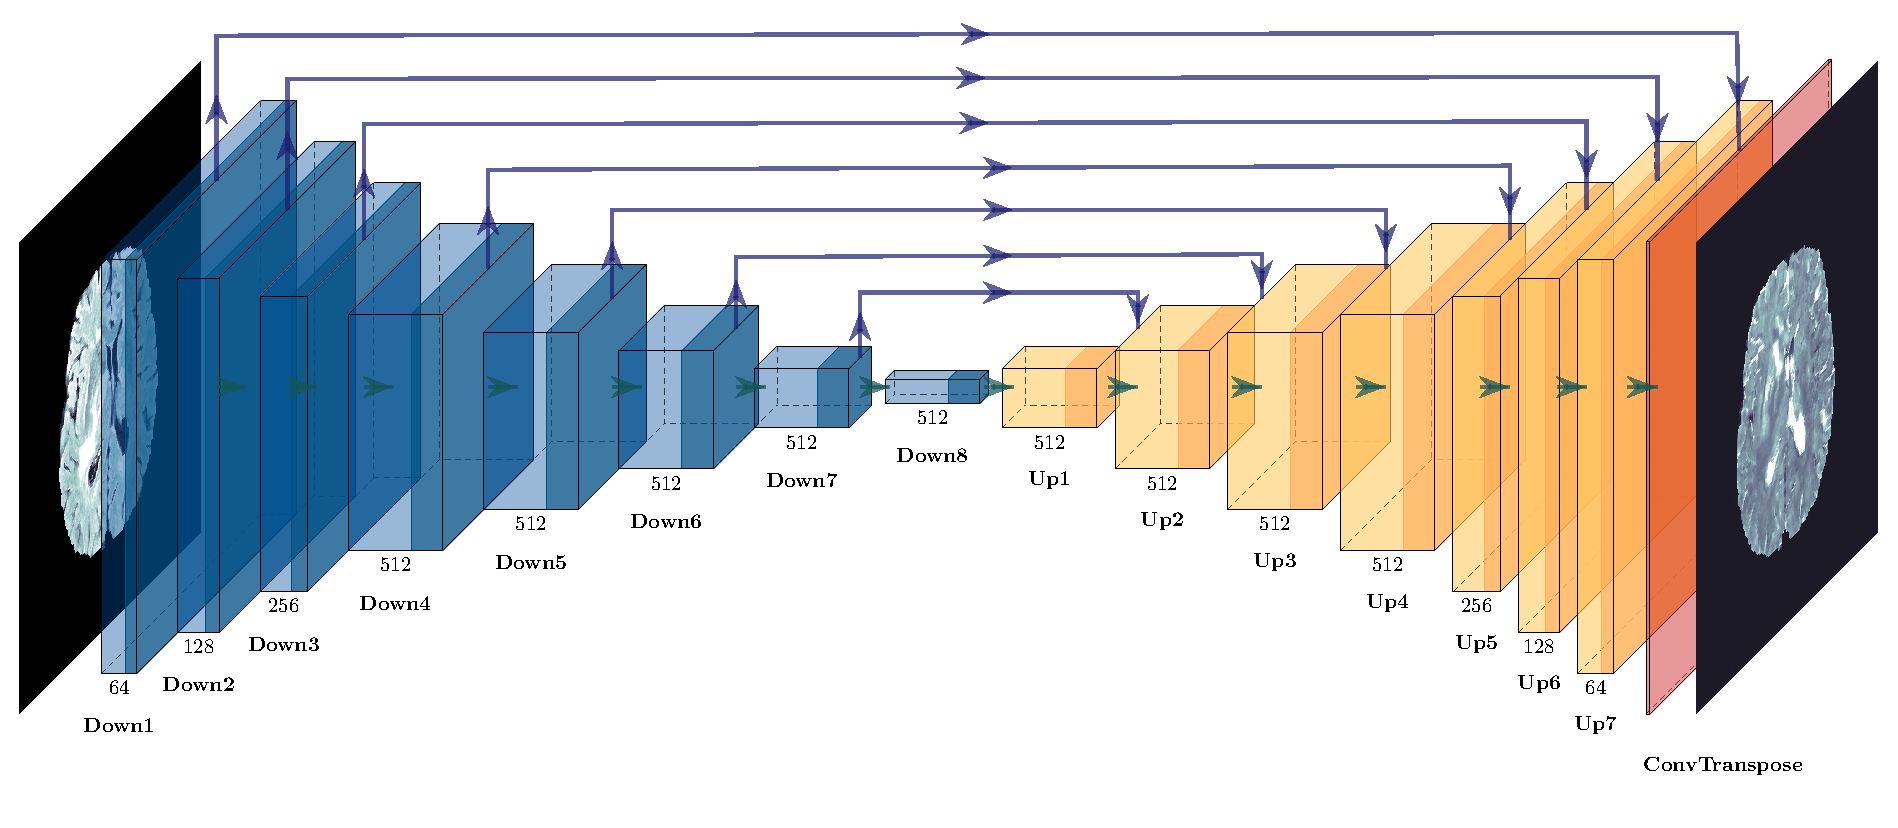
\includegraphics[height=0.266\textheight]{images/pix2pix_generator.pdf}
\caption[Generator architecture from pix2pix]{Generator architecture from pix2pix \cite{pix2pix}.}
\label{fig:pix2pix_generator}
\end{figure}

In Section \ref{sec:input_pipeline} we explained that it was necessary to add a padding to our images because otherwise they wouldn't have been compatible to the input of the images: the problem with U-Net comes from the nature of its mirrored architecture and more in particular from its downsampling and upsampling layers that allow to have only input images with dimensions that are power of 2. We choose then to pad our 180x180 images in order to obtain a width and height of 256, instead of applying a resize/crop to 128: transformation that wouldn't have preserved all the information in the images. 

\vspace{2mm} %5mm vertical space
The input fed to the model goes first through the contracting path: a typical convolutional neural network (Subsection \ref{sec:convolutional_neural_network}) composed by the repeated application of one the two main building blocks of the network, the \textbf{downsample block}, composed as follows:

\begin{itemize}
\item \textbf{Convolution}, that halves the dimensions of the input by convolving it through several filters with a fixed kernel size equal to 4 and stride of 2 for all the spatial dimensions.
\item \textbf{Batch Normalization} in every block (with the exception of the first one). This operations zero-centers and normalizes each input, trying to overcome to the problem of the vanishing gradient \cite[p.~728]{hands_on_ml}.
\item \textbf{Leaky ReLU}, an activation function similar to ReLU but with a small slope for negative values useful to avoid that some neurons "die" during training (meaning that they stop outputting anything other than 0) \cite[p.~720]{hands_on_ml}.
\end{itemize}
The repeated downsampling reduces the spatial information while increases the feature dimension, until the input arrives at the bottleneck where the output shape of the last downsampling block (\textit{Down7}) is [1x1x512].

\vspace{2mm} %5mm vertical space
The building block that characterizes the expanding path of the network is instead the \textbf{upsample block}, composed by four layers:

\begin{itemize}
\item \textbf{Transposed convolution} that goes in the opposite direction of what is done by the Convolution, by enlarging the spatial information: image is first stretched with the insertion of empty rows and then a regular convolution is computed. A kernel size of 4 and stride of 2 was set in this layer.
\item \textbf{Batch Normalization}
\item \textbf{Dropout}, useful for its regularization effect against some possible overfitting, it was applied in the first three upsampling blocks.
\item \textbf{ReLU} that has the advantage to not saturate for positive values (and it is fast to compute) \cite[p.~720]{hands_on_ml}
\end{itemize}

The last layer in the architecture of the generative part of \cite{pix2pix} is another transposed convolution that prepares the output of the model with tanh (hyperbolic tangent) as activation function, that returns values in a range between -1 and +1.
The output of the network is a batch of images, 32 in our case, with dimension 256x256x1.

\vspace{6mm} 
\noindent\textbf{Discriminator}

\vspace{2mm}
\noindent The PatchGAN \cite{patchgan} used to distinguish true images from fake images is similar to the well-known Convolutional Neural Network architecture (Section \ref{sec:convolutional_neural_network}), with the difference that the discriminator of pix2pix doesn't discriminate the whole image but small \textit{N}x\textit{N} patches of the input image: in this way the network can focus on capturing high frequencies details and assign to each patch a fake or true label. 

This means that the output of the discriminator we used, in pix2pix and in the other \ac{GAN}s we experimented with, isn't a 1x1 value but a 30x30 matrix, where each value contains the result of the discrimination over a 70x70 portion of the input image (the authors that developed \cite{pix2pix} suggest to use a patch of this size to obtain the best results from the \ac{GAN}).

\vspace{2mm} %5mm vertical space
Because of this, the network used is called 70x70 PatchGAN and takes two inputs, as illustrated in Figure~\ref{fig:pix2pix_discriminator}, each with shape [32, 256, 256, 1]: the first one is an input image while the second one is the target that can be an image coming from the dataset or a sample  generated by the \ac{GAN}. 

\begin{figure}[H]
\centering
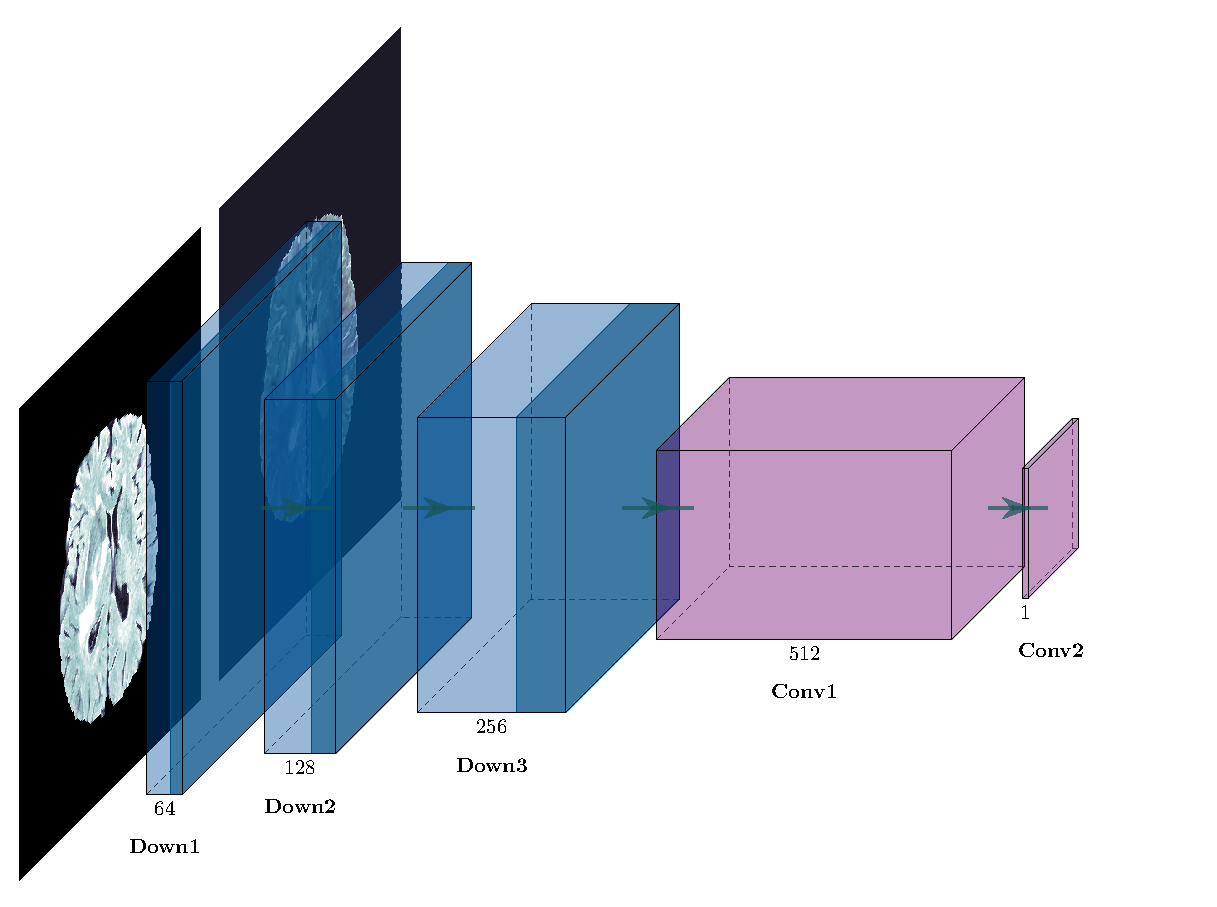
\includegraphics[height=0.3\textheight]{images/pix2pix_discriminator.pdf}
\caption[Discriminator architecture from pix2pix]{Discriminator architecture from pix2pix \cite{pix2pix}.}
\label{fig:pix2pix_discriminator}
\end{figure}

\vspace{2mm} %5mm vertical space
The discriminator architecture, differently from the one of the generator, has only a contracting path and is composed by three downsample blocks that allow to reduce the spatial dimensions of the image while increasing the feature dimension. Each one of these blocks is characterized by a different number of filters (64 the first block, 128 the second one and 256 the last one) and they are defined with the same layers that compose a downsample block in the generator (so batch normalization applied only in \textit{Down2} and \textit{Down3}.


These blocks are then followed by several layers: 

\begin{itemize}
\item \textbf{Zero Padding}, that doesn't increment the number of trainable parameters, because it simply adds zeros at the top, left, right and bottom of an image.
\item \textbf{Convolution} with 512 filters, kernel size equal to 4 and stride of 1.
\item \textbf{Batch Normalization}
\item \textbf{Leaky ReLU}
\item \textbf{Zero Padding}
\item Final \textbf{convolution} with 1 filter, again with kernels of 4x4 and stride set to 1.
\end{itemize}

\noindent The description of the training algorithm used by pix2pix can be found in Subsection \ref{subsec:training_algorithm} while the implementation details are discussed in Subsection \ref{subsec:implementation_details}.

\subsection{MI-pix2pix}
\label{subsec:mi_pix2pix_architecture}
MI-pix2pix is the second Generative Adversarial Network that we included in our experiments: it is a modified version of pix2pix \cite{pix2pix} adapted to a multi-input scenario in order to compare and evaluate the differences between an unimodal approach and its variant that takes multiple modalities of available information as input.

\vspace{6mm} 
\noindent\textbf{Generator}

\vspace{2mm}
\noindent The layers that compose the generator architecture (Figure~\ref{fig:MIpix2pix_generator}) are the same as the ones that define the pix2pix model with the only difference in the input shape, that is set to [32, 256, 256, 3], while the output shape remains equal to [32, 256, 256, 1]. For example a MI-pix2pix that has to synthesize the missing $T_{2}$ sequence of a subject will use the information from the other three modalities available: $T_{1}$, $T_{1c}$, $T_{flair}$ that are the inputs respectively of the first, second and third input channel.

\vspace{6mm} 
\noindent\textbf{Discriminator}

\vspace{2mm}
\noindent Also for the Discriminator we maintained the same architecture (Figure~\ref{fig:MIpix2pix_discriminator}) used in the unimodal version of pix2pix, but, since we are in a multi-modal setting, while the target has still a shape of [32, 256, 256, 1], the second input is a concatenation of the three modalities ([32, 256, 256, 3]) used to feed also the Generator.

\begin{figure}[H]
\centering
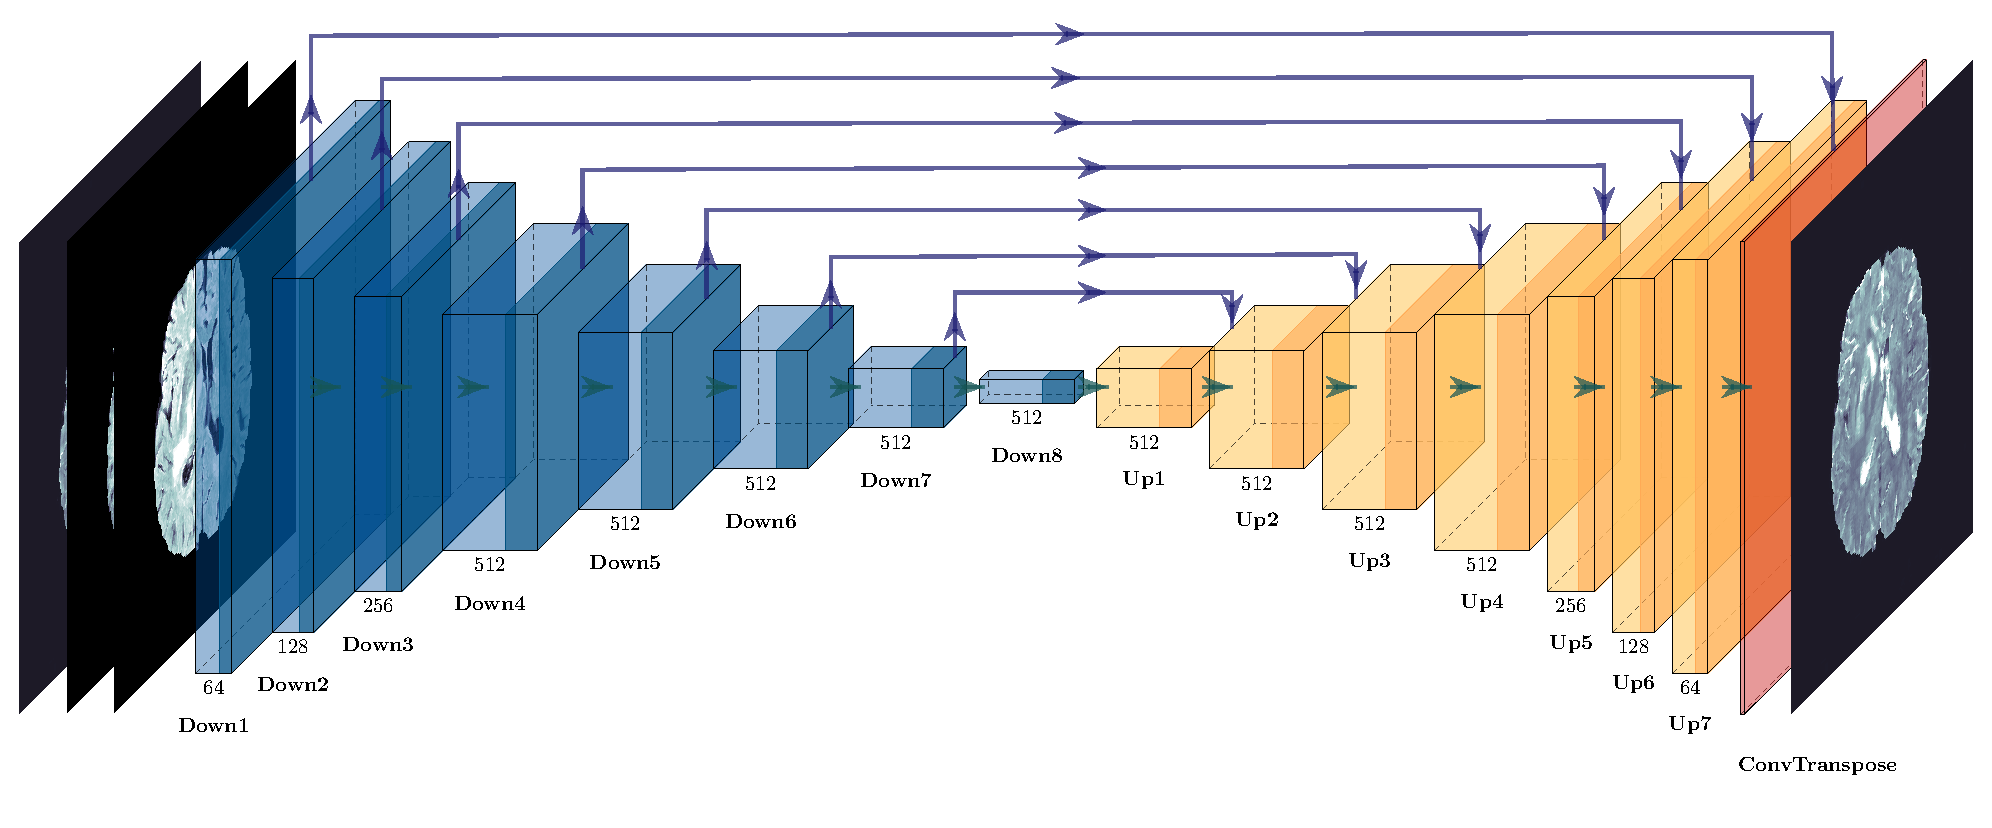
\includegraphics[height=0.263\textheight]{images/MIpix2pix_generator.pdf}
\caption[Generator architecture from MI-pix2pix]{Generator architecture from MI-pix2pix.}
\label{fig:MIpix2pix_generator}
\end{figure}

\begin{figure}[H]
\centering
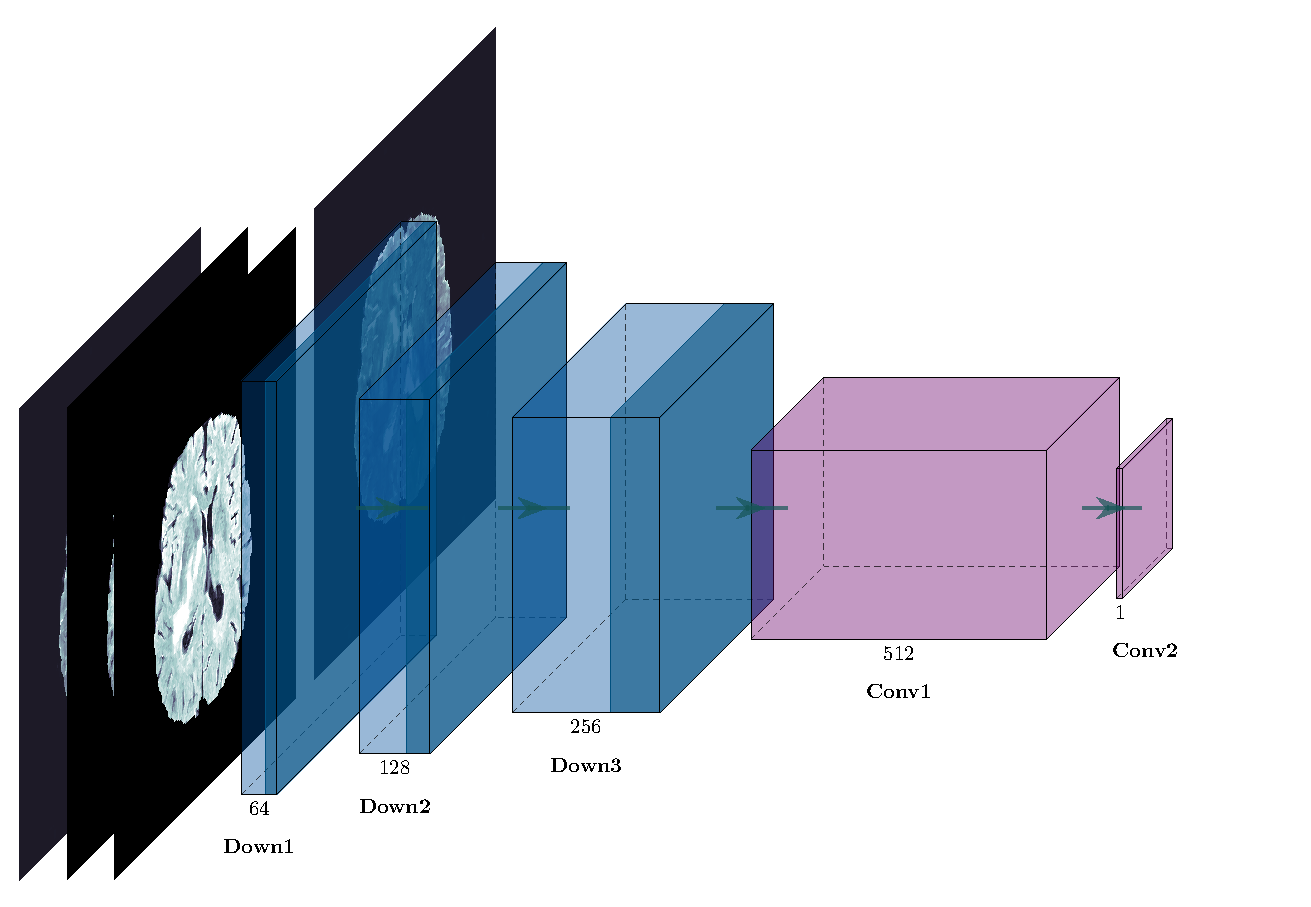
\includegraphics[height=0.335\textheight]{images/MIpix2pix_discriminator.pdf}
\caption[Discriminator architecture from MI-pix2pix]{Discriminator architecture from MI-pix2pix.}
\label{fig:MIpix2pix_discriminator}
\end{figure}



\noindent MI-pix2pix was very useful to understand whether a multi-modal approach can exploit the information coming from different \ac{MRI} sequences in a better way than what is done by pix2pix, since the two \ac{GAN}s share the same architecture and the same layers but receive a different number of images. The results of the comparison are presented in Chapter \ref{cha:5th_chapter}.

\vspace{2mm} %5mm vertical space
As for pix2pix, description of the training used can be found in Subsection \ref{subsec:training_algorithm} while the implementation details are discussed in Subsection \ref{subsec:implementation_details}.

\subsection{MI-GAN}
\label{subsec:mi_gan_architecture}
The third Generative Adversarial Network that we implemented is a multi-modal approach inspired by the work of Anmol Sharma and Ghassan Hamarhneh that in 2019 presented a multi-input multi-output \ac{GAN}, called MM-GAN, that seems to be, to the best of their knowledge, the first method capable of synthesizing multiple missing sequences using a combination of various input sequences (many-to-many) \cite{migan}.

\vspace{2mm} %5mm vertical space
Since the core of this work is on the generation of a single-output image, using different configurations and architecture of \ac{GAN}s, we focused our attention on a modified version multi-input single-output (many-to-one) of MM-GAN, called MI-GAN and implemented also by Sharma and Hamarhneh.

The focus of \cite{migan} was on the many-to-many approach though, and as a consequence many details about the MI-GAN model weren't given: because of this, our model was inspired by the MM-GAN but at the same time it presents some variations that we applied, both to the architecture and to the loss used in the training algorithm (Subsection \ref{subsec:training_algorithm}), in order to obtain a more stable training and satisfiable results in the generated samples.

\vspace{2mm} %5mm verticalspace
The layers that define the architecture of MI-GAN are almost the same proposed in \cite{migan} for the MM-GAN: the only variation applied was the replacement of every layer of Instance Normalization with a Batch Normalization, used also in pix2pix (Subsection \ref{subsec:pix2pix_architecture}) and in MI-pix2pix (Subsection \ref{subsec:mi_pix2pix_architecture}), after observing through various experiments that normalizing the activations of each channel across the whole batch was more effective, in terms of quality in the generated samples, instead of computing the mean/standard deviation and normalizing across each channel in each training image.

\vspace{6mm} 
\noindent\textbf{Generator}

\vspace{2mm}
\noindent The generator is a modified U-Net with concatenated skip connections and the typical U-shape architecture (Figure~\ref{fig:MIGAN_generator}), characterized by two known building blocks: one that downsamples its input and one that, through a transposed convolution, performs an upsampling. 

The \textbf{downsample block} is composed in a similar way to the one used in the previous model, with the addition of a dropout layer at the end of the block.

\begin{itemize}
\item \textbf{Convolution} with kernel size equal to 4 and stride of 2.
\item \textbf{Batch Normalization} in every block beside the first one.
\item \textbf{Leaky ReLU}
\item \textbf{Dropout} with the rate defining the fractions of the input dropped to 0, at each update during training time, set to 0.5. 
\end{itemize}

\begin{figure}[H]
\centering
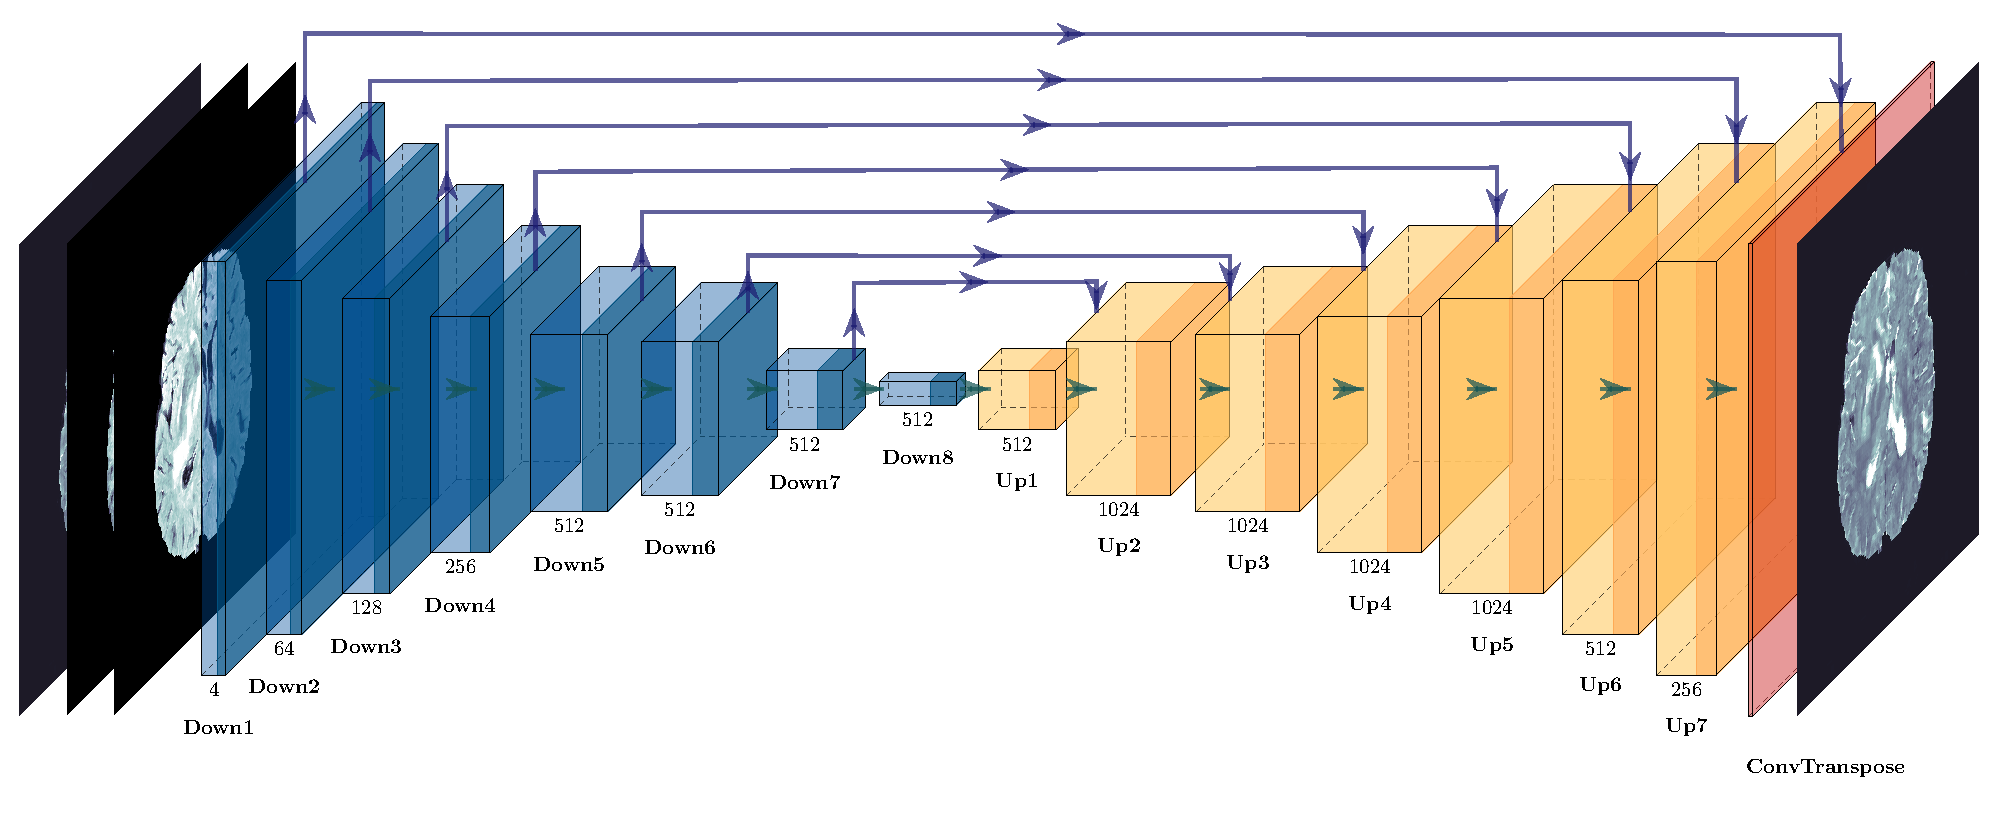
\includegraphics[height=0.263\textheight]{images/MIGAN_generator.pdf}
\caption[Generator architecture of MI-GAN]{Generator architecture of MI-GAN.}
\label{fig:MIGAN_generator}
\end{figure}

The \textbf{upsample block} instead, following the MM-GAN architecture, has the same layers seen in the pix2pix architecture with the difference that the dropout layer is applied after the ReLU activation function:

\begin{itemize}
\item \textbf{Transposed Convolution}
\item \textbf{Batch Normalization}
\item \textbf{ReLU}
\item \textbf{Dropout} (with 0.5 rate) applied to the first three upsample blocks.
\end{itemize}

At the end of the network, after the last upsample block, a transposed convolution with tanh as activation function is used to reduce the feature dimension and to enlarge the spatial dimensions of the image from 128x128 to the final shape of 256x256.

\vspace{5mm} %5mm vertical space
Regarding the problem of how many input and output channels use in the generator, we performed two experiments with the architecture above defined: in the first one, following \cite{migan} and adapting the MM-GAN network from a many-to-many to a many-to-one scenario, we trained a generator to produce 4 different modalities (but only the synthesized image of the missing sequence was used to compute the loss, while the other three were discarded) receiving as input a concatenation of 4 images.
These images given as input, in the case for example of $T_{1}$ missing, were the three remaining modalities \{$T_{2}$, $T_{1c}$, $T_{2flair}$\} and a zero-value image through the channel of the missing sequence (so the channel of $T_{1}$ was obscured).
The second approach we tested was about using a generator with the same input and output shape already used in MI-pix2pix: a single image with shape [32, 256, 256, 1] generated by a model that receives three 32x256x256 different modalities.

\vspace{5mm} %5mm vertical space
The results obtained led us to discard the first solution, probably more functional in a many-to-many scenario, and to choose the second approach that outperformed the other one both in a qualitatively (human perception of quality from the generated samples) and quantitatively (scores from the similarity/error metrics applied to the synthesized images) way.

\vspace{6mm} 
\noindent\textbf{Discriminator}

\vspace{2mm}
\noindent The experiments we did in order to find the best suitable network involved also the Discriminator: with the generator synthesizing 4 images, we implemented the model discussed in \cite{migan} that takes two inputs $X_t$ and $X_i$ and produces one output D($X_t$, $X_i$), each one of these with 4 channels, one per modality: assuming the discrimination of a $T_{1}'$ synthesized scan, the inputs were $X_t$: \{$T_{1}$, $T_{2}$, $T_{1c}$, $T_{2flair}$\} and $X_i$: \{$T_{1}'$, $T_{2}$, $T_{1c}$, $T_{2flair}$\}.

In second experiment, the one with the generator producing only one image, the two discriminator inputs, input and target, had respectively shape [32, 256, 256, 3] and [32, 256, 256, 1] with an output with dimensions equal to 32x15x15x1 (in the discrimination of a $T_{1}'$ scan, the inputs were \{$T_{2}$, $T_{1c}$, $T_{2flair}$\} and $T_{1}'$).
As said before, we choose to use the second solution, over the first one.

\vspace{5mm} %5mm vertical space
The discriminator is a PatchGAN \cite{patchgan} composed by four downsampling steps called \textbf{discriminator blocks}, similar to the ones used by the MM-GAN {\cite{migan}}. Each block contains, in order, the following layers:

\begin{itemize}
\item \textbf{Convolution}, with a number of filters ranging from 64 (first block) to 512 (last block).
\item \textbf{Batch Normalization} applied in the second, third and fourth block.
\item \textbf{Leaky ReLU}
\end{itemize}

At the end of these sequence of blocks, two more layers are applied (Figure~\ref{fig:MIGAN_discriminator}):

\begin{itemize}
\item \textbf{Zero Padding}
\item Final \textbf{Convolution} with kernel size to 4 and strides set to 1.
\end{itemize}

\noindent The description of the training algorithm as well as the loss formulation used by MI-GAN is in Section \ref{sec:training}, while the implementation details are discussed in Subsection \ref{subsec:implementation_details}.

\begin{figure}[H]
\centering
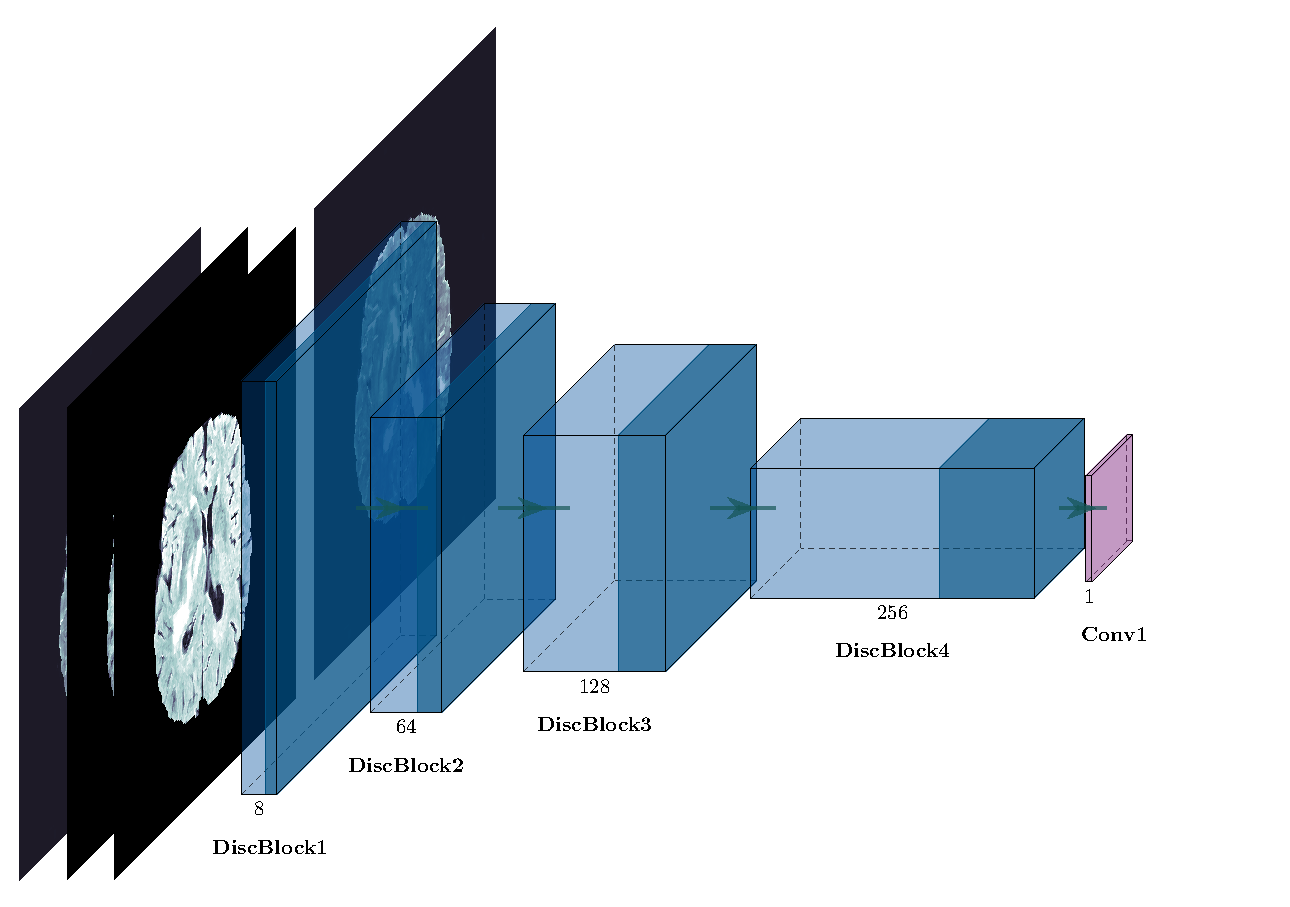
\includegraphics[height=0.335\textheight]{images/MIGAN_discriminator.pdf}
\caption[Discriminator architecture of MI-GAN]{Discriminator architecture of MI-GAN.}
\label{fig:MIGAN_discriminator}
\end{figure}

\section{Training}
\label{sec:training}
In a Generative Adversarial Network, generator and discriminator are trained simultaneously using \textit{Backpropagation}, with D that learns to recognize the true images from the fake ones and G that, based on the feedback received by the first neural network, learns to produce more realistic images in order to be able to fool D. In this adversarial setting, the competing behaviour of one against each other is defined by two different loss functions.

\subsection{Loss Formulation}
\label{subsec:loss_formulation}
The generator loss and discriminator loss used with MI-GAN (\ref{subsec:mi_gan_architecture}) are the ones proposed in \cite{pix2pix} and defined as follows: 

\begin{equation} \label{eq:losses_migan}
\begin{gathered}
L_G\leftarrow \lambda\mathcal{L}_{1}(G(x), y) + (1 - \lambda) \mathcal{L}_{2}(D(x, G(x)), L_{ar})  \\
L_D \leftarrow \mathcal{L}_{2}(D(x, y), L_{ar}) + \mathcal{L}_{2}(D(x, G(x)), L_r) 
\end{gathered}
\end{equation}

where $x$, the input, is a concatenation of three sequences while $G(x)$ represents the prediction generated by the \ac{GAN}.
$L_{ar}$ is a dummy ground truth tensor that is used by the generator loss to fool the discriminator by setting all the entries to one, in such a way that G is encouraged to generate modalities that can fool D.

$\mathcal{L}_{2}$ is the L2 norm (also known as mean squared error) while $\mathcal{L}_{1}$ instead is the mean absolute error (L1 norm) that is useful to the generated image because it allows to become structurally similar to the target image. This term was chosen as reconstruction loss term because of its ability to prevent too much blurring, as compared to using a L2 loss \cite{migan}.
$L_r$ is instead a tensor with its entries equal to zero, useful for D to distinguish the fake samples (associated to 0, by using $L_{r}$) from the true samples (associated to 1 through $L_{ar}$).

\vspace{5mm} %5mm vertical space
Pix2pix (\ref{subsec:pix2pix_architecture}) and MI-pix2pix (\ref{subsec:mi_pix2pix_architecture}) share the same objective function (Eqn.~\ref{eq:final_objective}), since they have an identical architecture and the only difference between the models is in the number of inputs that their generator can receive.

In the implementation of these two networks, we applied the same losses that are used in \cite{pix2pix_implementation}, similar to the ones adopted in the MI-GAN training algorithm: here, a binary crossentropy is used instead of the L2 term. 

The $L_D$ of pix2pix and MI-pix2pix is computed as the sum between the binary crossentropy of $(D(x,y), L_{ar})$ and the one of $D((x, y'), L_{r})$ where $y'$ is the generated image.
$L_G$, on the other hand, contains the reconstruction term between $y$ and $y'$, multiplied by an hyper parameter lambda and summed to the binary crossentropy of $D((x, y'), L_{r})$.

\subsection{Training Algorithm}
\label{subsec:training_algorithm}
Due to some implementation needs and to be able to define our own metrics (Section \ref{sec:evaluation_metrics} for details) and losses, we wrote a custom train step (where is contained the update of the weights) as well as evaluation loops instead of using the built-in training optimized by \textit{Tensorflow}. The two approaches work strictly in the same way across every kind of \textit{Keras} model, but implementing everything from scratch allowed us to have a lower-level training and full control on the evaluation step, as well as the possibility to being able to retrieve all the gradients of the trainable weights of a layer with respect to the loss.  

For implementing the training algorithm we followed the algorithm applied in \cite{pix2pix_implementation}, which uses \textit{Adam} \cite{kingma2014adam}, an adaptive learning rate method, as optimizer for both the networks.

\vspace{5mm} %5mm vertical space
During the training of our models, we didn't make use of the regularization technique called \textit{Early Stopping}, used to prevent overfitting in many \ac{DL} methods. This technique is based on the idea of stopping the training procedure before the model starts to overfit, by looking at the performances on the validation set, in particular at the validation loss: when its value, after an initial improvement of the learner's ability to generate/predict/classify, starts to increase, it means it is probably the right moment to stop the training because the models is incurring into a larger generalization error. In our case though, we observed that, often, after an abrupt increase of one of the two losses, the networks after few epochs were returning to a stable training level, without the need of killing the procedure and restarting again from the beginning. 

\begin{figure}[H]
\centering
\includegraphics[height=0.331\textheight]{images/loss_behaviour2.pdf}
\caption[Validation loss during MI-GAN training]{Typical behaviour of the validation losses through the epochs of MI-GAN training.}
\label{fig:loss_behaviour}
\end{figure}

Furthermore, our Generative Adversarial Networks continued to improve the overall quality of their generated image even if their losses values, the indicators used to understand when we should stop, had been stable for 10, 20, even 30 epochs: \ac{GAN}s took long time to train and long time to show some progress in the synthesized samples, that's why it was important to wait for a while before killing the training. The only exception is represented by the case in which the loss went rapidly to 0, sign that something wasn't working in the proper way and that the network had incurred in a failure to converge, that can happen for example when the discriminator loss drops to 0 because it is learning more rapidly with respect to the generator.

\vspace{5mm}
Figure~\ref{fig:epochs_behaviour} illustrates the differences between the original $T_{1c}$ slice and its prediction, from MI-GAN, after 5 and 20 epochs of training: it shows how much a \ac{GAN} can improve the quality of the generated images, adding low-level details and reducing the overall blurriness, even when the losses, both in the generator and in the discriminator, are not improving over time (Figure~\ref{fig:loss_behaviour}): proof that, during training, a visual understanding is much more meaningful than just looking at the values of the losses.


\begin{figure}[H]
\centering
\includegraphics[height=0.56\textheight]{images/t1c_through_epochs.pdf}
\caption[$T_{1c}$ predictions from MI-GAN]{Prediction of $T_{1c}$ slices on the validation set, using MI-GAN.}
\label{fig:epochs_behaviour}
\end{figure}
\newpage
\subsection{Implementation Details}
\label{subsec:implementation_details}

The hyperparameters used are the learning rate $\alpha$ set to 0.0002 and the exponential decay rate for the 1st moment estimates $\beta_1$ equal to 0.5 while the one for the 2nd moment estimates ($\beta_2$) was left to the default value of 0.999.

$\lambda$ has a value of 100 in the generator loss of pix2pix and MI-pix2pix, while is set to 0.9 in the loss of the MI-GAN generator. 
The MI-GAN discriminator loss instead is multiplied by 0.5, choice motivated by the need to slow down the rate at which D learns compared to G.

\vspace{5mm} %5mm vertical space
Furthermore, the transposed convolution layers in the generators architectures (whose shapes are summarized in Table~\ref{tab:resume_architectures_generators}) as well as the convolutions used by both generators and discriminators (Table~\ref{tab:resume_architectures_discriminators}) have a variable number of filters with dimension 4x4 and with kernel weights initialized using a normal distribution with 0 mean and standard deviation equal to 0.05.

\begin{table}[htbp!]
\centering
\begin{tabular}{ccc}
\toprule
Model & Inputs & Output\\
\midrule
pix2pix Generator & [32, 256, 256, 1] & [32, 256, 256, 1]\\
MI-pix2pix Generator & [32, 256, 256, 3] & [32, 256, 256, 1]\\
MI-GAN Generator & [32, 256, 256, 3] & [32, 256, 256, 1]\\
\bottomrule	
\end{tabular}
\caption[Generators input and output shapes used during training]{Generators input and output shapes used during training. 32 is the batch size we choose to use. The last input dimension is the number of channels, so it represents how many modalities can be fed to the model.}
\label{tab:resume_architectures_generators}
\end{table}

\begin{table}[H]
\centering
\begin{tabular}{ccc}
\toprule
Model & Inputs & Output\\
\midrule
pix2pix Discriminator & [32, 256, 256, 1],[32, 256, 256, 1] & [32, 30, 30, 1]\\
MI-pix2pix Discriminator & [32, 256, 256, 3],[32, 256, 256, 1] & [32, 30, 30, 1]\\
MI-GAN Discriminator & [32, 256, 256, 3],[32, 256, 256, 1] & [32, 15, 15, 1]\\
\bottomrule	
\end{tabular}
\caption[Discriminators input and output shapes used during training]{Discriminators input and output shapes used during training.}
\label{tab:resume_architectures_discriminators}
\end{table}

Python 3.6.9 is the main programming language of our work. We used \cite{pix2pix_implementation} as reference for the implementation of the pix2pix model that, as MI-pix2pix and MI-GAN, was built using mainly the library of Tensorflow 2.1.0. For our experiments we used \href{https://colab.research.google.com}{Google Colaboratory}, a hosted Jupyter notebook service, that offers free usage of its computing hardware consisting of a Tesla P100-PCIE-16GB GPU with 26 GB of RAM available and an Intel(R) Xeon(R) CPU @ 2.30GHz.
\newpage
\section{Evaluation Metrics}
\label{sec:evaluation_metrics}
In \autoref{subsec:training_algorithm} we discussed about how much is important to evaluate an image in a qualitatively way, by looking not only at the losses values reached by the networks through the epochs in the training phase but also at the quality of the generated samples. 
Beside the qualitative measure though, it was necessary to define some quantitative metrics that were able to understand how much error and similarity there were between our prediction and the original image. 

\vspace{5mm} %5mm vertical space
These metrics resulted particularly useful during training when there wasn't any visible difference in the quality of the synthesized modalities between two epochs as well as, on the other hand, human perception was very effective in the cases of images, from different epochs, with almost same values but with a clear difference in low-level details that the metrics couldn't capture.

\subsection{Evaluation of the Whole Image}
\label{subsec:eval_overall_area}
The first metrics we implemented were the ones to evaluate the whole area of the images produced by the \ac{GAN}s. In order to obtain results as more accurate as possible, we proceeded to crop and normalize both the prediction and the original image: we center-cropped the generated images of size 256x256 to the dimensions of 155x194, after calculating the largest bounding box able to contain each brain of the dataset \cite{migan}. 

This was motivated by the fact that computing, for example, the similarity between two images padded to have compatible size with the input of the networks returns a much higher value than the one obtained comparing two 155x194 slices: an high value due to the presence of many black pixels that risks to bias the performances on the metrics (Figure~\ref{fig:before_after_crop}).

\begin{figure}[H]
  \centering
  \subfloat{\includegraphics[height=0.24\textheight]{images/256x256.pdf}
  \label{fig:f1}}
  \hspace{1.6cm}
  \subfloat{\includegraphics[height=0.145\textheight]{images/155x194.pdf}\label{fig:f2}}
  \caption[$T2$ slice before and after crop to 155x194]{$T2$ slice before and after crop to 155x194, applied to remove as many not relevant pixels as possible before the calculation of the metrics.}
  \label{fig:before_after_crop}
\end{figure}

\vspace{5mm} %5mm vertical space
In order to obtain consistent results during the comparison and avoid to compute a metric between an original image that has intensity values ranging from 0 to 1 and a predicted image with a different range, happening especially during the evaluation of the model in the first epochs of the training (while at the end of the training the \ac{GAN} learns to synthesize images that lie in the same normalized range of the input image), we proceeded to apply a scaling.

The transformation applied to the original image and to its prediction is a \textbf{mean normalization}, whose formula, taken from \cite{mean_norm}, is the following:

\begin{equation} \label{eq:mean_normalization}
x' = \dfrac{x - \mathrm{average(x)}}{\max(x) - \min(x)}
\end{equation}

where \textit{x} is the original value, \textit{x'} is the normalized value. This method, similar to the min-max, allows the pixels to have approximately zero mean and dynamic range equal to 1. 

Differently from the normalization done, in the preprocessing step (Section \ref{sec:preprocessing}), to the whole volume, here the transformation is applied with respect to the slice (the min and max values are respectively the minimum and maximum intensity values of the slice, not of the whole volume). We didn't normalize with respect to the volume because our \ac{GAN}s are trained to predict a single image based on a single slice: therefore we considered this approach as a better method to evaluate our predictions.

%The metrics implemented to evaluate the overall area of the brain consider in the calculations not only the pixels relative to the brain but also the ones with zero-value: even if removing all the black pixels wouldn't have been wrong, we preferred the first approach since the \ac{GAN} generates 

\vspace{6mm} 
\noindent\textbf{Mean Squared Error}

\vspace{2mm}
\noindent Mean Squared Error (MSE), one of the metrics that we implemented, allows to estimate the error between its inputs. More specifically, MSE measures the average squared difference between the estimated pixels values and the intensity values belonging to the true image. It is computed as:

\begin{equation} \label{eq:mse}
MSE =  \frac{1}{N} \sum_{i=1}^{N} (y_i - y'_i)^2
\end{equation}

where $y_i$ is the original image while $y'_i$ is the synthesized image. 

To implement it, we used a function from the library of Tensorflow that computes a MSE per each pixel in the image (that is the same of doing just a squared difference between the true pixel and the predicted pixel, since N = 1). The function returns a matrix 155x194, whose values are then averaged to obtain the final mean squared error between $y_i$ and $y'_i$.

\newpage
\noindent\textbf{Peak Signal-to-Noise Ratio}

\vspace{2mm}
\noindent Peak signal-to-noise ratio, often abbreviated PSNR, is a metric that computes, in decibels (dB), the ratio between the maximum intensity value allowed in the image \cite{psnr} and the MSE and is defined as:

\begin{equation} \label{eq:psnr}
PSNR =  10\log_{10} \frac{I^2_{max}}{MSE}
\end{equation}

where $I_{max}$ is the dynamic range that corresponds to the maximum intensity value of the image when its range is [0, 1].
The higher the PSNR, the better is the quality of the predicted image, since the ratio has a measure of error, the MSE, as denominator. For the implementation of this metric we used a built-in function from Tensorflow that receives two images and directly computes the PSNR value.

\vspace{6mm} 
\noindent\textbf{Structural Similarity}


\vspace{2mm}
\noindent This metric is defined as the structural similarity (SSIM) index between two images, designed to improve on traditional metrics such as Mean Squared Error and Peak Signal-to-Noise Ratio. 
SSIM ranges from 0 to 1 and is a metric that doesn't compare the images just on a single statistic: its value of similarity is based on different factors such as the luminance, the contrast and the structure. Furthermore, the structural similarity is applied locally over the image due to the fact that pixels spatially close are the ones with stronger inter-dependencies, somehow similar to the way in which human perception works. SSIM is computed as:

\begin{equation} \label{eq:ssim}
SSIM =  \frac{(2\mu_x + \mu_y + c_1)(2\sigma_{xy} + c_2)}{(\mu^2_x + \mu^2_y + c_1)(\sigma^2_x + \sigma^2_y + c_2)}
\end{equation}

where $x, y$ are the two images to be compared, $\mu$ is the mean intensity, $\sigma^2$ the variance of the image and $\sigma_{xy}$ the covariance of $x, y$.

\vspace{5mm} %5mm vertical space
For calculating this metric we used the implementation provided by the Tensorflow library which in turn is based on the standard SSIM implementation from \cite{ssim}. The only parameter that we needed to specify was the dynamic range of the images (difference between the max and min allowed values), that in our case, thanks to the mean normalization, is equal to 1. 

The SSIM reported in Chapter \ref{cha:5th_chapter} are obtained by computing the mean and standard deviation over all the SSIM values calculated by comparing each original image in the test test with its prediction. 

\subsection{Evaluation of the Tumor Area}
\label{subsec:eval_tumor_area}

The most relevant part of the brain, to us and in general to the doctors that have to make a diagnosis, is the tumor. Because of this we implemented three more ways in which we could evaluate the results of our predictions, not anymore by looking at the whole brain area but by focusing on the tumor. 

The exact information of which pixels belong to the tumor and which do not is contained in the \textit{Ground Truth} volumes that show the segmentation of the malignant area of the brain.

\vspace{6mm} 
\noindent\textbf{MSE and PSNR} 

\vspace{2mm}
\noindent To compute the performances on the tumor area we implemented a modified version of the metrics used to evaluate the whole area: MSE and PSNR.
To do this, we had first to use the ground truth as a mask to isolate the interested area by setting to 0 all the pixels belonging to the healthy part of the brain.
Figure~\ref{fig:brain_masked} illustrates the result obtained by masking a $T_{2flair}$ slice with its ground truth.

\begin{figure}[H]
\centering
\includegraphics[height=0.30\textheight]{images/brain_tumor_masked.pdf}
\caption[$T_{2flair}$ slices masked with the ground truth]{$T_{2flair}$ slices and their masked versions, using the ground truth.}
\label{fig:brain_masked}
\end{figure}

After scaling with mean normalization (\ref{eq:mean_normalization}) and masking both the original image and the predicted missing modality with the ground truth, we proceeded to measure the quality of the images with the modified versions of MSE and PSNR.

\vspace{5mm} %5mm vertical space
The idea was to modify the MSE (and so the PSNR, that depends on the MSE) by including in the calculation only the pixels belonging to the tumor area, so without considering the pixels corresponding to the back pixels in the ground truth image.

It was necessary to not consider all these black pixels because they would have affected (and boosted) the metrics of similarity, by reaching higher values, as well as the error metrics, by dropping significantly to values close to 0.

We then computed the MSE between the masked images (target masked and prediction masked) by dividing the squared difference by the number of pixels in the ground truth with value different from 0, instead of dividing by the total number of pixels in the whole image. It was sufficient to apply only this slightly variation to the MSE Formula (\ref{eq:mse}), since the squared difference value wasn't affected by the presence of the black pixels: both the masked images had zero intensity in the dark area, resulting in a difference of values equal to 0.

\vspace{5mm} %5mm vertical space
It is also important to highlight that, even if every patient has a tumor, not all the slices extracted from a volume contain a malignant area. Because of this, we didn't include in the calculations the slices whose masked images were completely black, since we are interested in evaluating only the generated area on the tumor: keeping all the masked slices would have boosted, again, the metrics.

\vspace{6mm} 
\noindent\textbf{Dice Similarity Coefficient}

\vspace{2mm}
\noindent To understand the quality of the generation process, beside the human perception and the other quantitative metrics implemented, we proceeded to evaluate our generated images using segmentation models that extract the tumor area from the synthesized missing modalities. 
In particular, we tested the result of the $T_{2flair}$ segmentation model from \cite{giacomello2019brain} using as input the $T_{2flair}$ predictions (with dimensions 256x256) obtained from our trained models (pix2pix, MI-pix2pix and MI-GAN).

\vspace{5mm} %5mm vertical space
The metric we implemented to evaluate the tumor segmentation model is the Dice similarity coefficient (DSC), also known as Sørensen–Dice coefficient, that measures the similarity between two images. DSC ranges from 0 to 1 and is defined as:

\begin{equation} \label{eq:dsc}
DSC =  \frac{2TP}{2TP + FP + FN}
\end{equation}

where TP (True positives) represents the number of pixels in the segmentation image correctly classified as belonging to the tumor while FP (False positives) is the number of pixels misclassified as positive. FN (False negatives) is instead the number of positive pixels in the ground truth that are classified as negative in the segmentation.
To implement this metric, we first counted the TP, FP, FN per every subject and from these values we calculated the DSC with respect to the volume, using \ref{eq:dsc}, and then we averaged the computed values of the 28 volumes (from the test set) to obtain the final score, reported in Chapter \ref{cha:5th_chapter}. Figure~\ref{fig:segmentation_example} shows the segmentation obtained from $T_{2flair}$ slices using a segmentation model \cite{giacomello2019brain}: the DSC is computed between the ground truth and the segmentation.

\begin{figure}[H]
\centering
\includegraphics[height=0.36\textheight]{images/segmentation_example.pdf}
\caption[Comparison between Ground Truths and Segmentations]{Comparison between Ground Truths and segmentations of $T_{2flair}$ slices obtained using the segmentation model from \cite{giacomello2019brain}.}
\label{fig:segmentation_example}
\end{figure}

\section{Summary}
\label{sec:4th_section_summary}
In this chapter we first discussed about the input pipeline optimization of our models. We proceeded then to present a detailed description about the architectures of the models we implemented: pix2pix, MI-pix2pix, MI-GAN.

We gave an overview of the training algorithm, of the losses used in the update step and the implementation details of this work in order to allow the reproducibility of our results.

At the end of the chapter is described how we evaluated the synthesized missing modalities obtained from the \ac{GAN}s in order to measure, as accurately as possible, the quality of the generation in both the tumor area and the whole area of the brain.
\chapter{Results}
\label{cha:5th_chapter}
In this chapter we report the results from our work: in Section \ref{sec:quantitative_results} are summarized the quantitative performances obtained by all the model trained, while in Section \ref{sec:qualitative_results} we illustrate, in a qualitative way, the ability of our \ac{GAN}s to synthesize MRI sequences, using the modalities contained in BRATS2015. 

In Section \ref{sec:results_evaluation} we provide our discussion on the results by considering them in the same order they are presented.

\section{Quantitative Results}
\label{sec:quantitative_results}

In this section we show the quantitative results reached by all the models we experimented with.
In total we trained 14 models using the three \ac{GAN}s presented in Chapter \ref{cha:4th_chapter}. Subsection \ref{subsec:t1_gen} shows the results obtained by four of these models, trained to generate $T_1$ slices.
In Subsection \ref{subsec:t2_gen} we present the ones relative to the generation of $T_2$ while Subsections \ref{subsec:t1c_gen} and \ref{subsec:t2flair_gen} contain the performances of the generative models trained to synthesize, respectively, $T_{1c}$ and $T_{2flair}$ slices. The tables reported in these subsections present three metrics used for the evaluation of the whole image, MSE, PSNR and SSIM, but also $\mathrm{MSE_{tumor}}$ and $\mathrm{PSNR_{tumor}}$, computed considering only the generated tumor area.

\vspace{5mm} %5mm vertical space
The pix2pix models (Subsection \ref{subsec:pix2pix_architecture}) are called P2P (where P2P$(T_{1c \rightarrow 1})$ is trained to generate $T_1$ from $T_{1c}$) while, for example, MI-P2P{$_{T_2}$} is the MI-pix2pix \ac{GAN} (Subsection \ref{subsec:mi_pix2pix_architecture}) generating ${T_2}$ from ($T_{1}$, $T_{1c}$, $T_{2flair}$).

\vspace{5mm} %5mm vertical space
Moreover, we introduced some baselines in order to understand if our single-input models were actually learning to generate a missing modality $y'$ or if, instead, they were only exploiting the similarities between the input and the output: basically we wanted to evaluate if there was more similarity between the generated image $y'$ and $y$ than between $x$ and $y$, in order to understand if the \ac{GAN} was correctly elaborating the image received in input. Therefore, Baseline$(x,y)$ corresponds to the values calculated by applying the metrics between modality $x$ and modality $y$.

In the tables of the following subsections, values in boldface represent best performance values. The reported values are mean $\pm$ std.

%%%%%%%%%%%%%%% T1 generation %%%%%%%%%%%%%%%%
\subsection{Generation of \texorpdfstring{${T_1}$}{TEXT}}
\label{subsec:t1_gen}

Four models were trained to generate the missing modality $T_1$: two unimodal \ac{GAN}s with different inputs ($T_2$ and $T_{1c}$) and two multimodal models. We choose to train different pix2pix models to understand how much good could have performed a single-input network that receives an image highly similar to the target ($T_{1c}$) compared to $\mathrm{P2P \ (T_{2 \rightarrow 1})}$.
The results are presented in Table \ref{tab:t1}.

\begin{table}[H]
\centering
\fontsize{8}{18}\selectfont
\setlength{\tabcolsep}{3.2pt}
\begin{tabular}{l|c|c|c|c|c}
\toprule
\textbf{Model} & \textbf{MSE} & \textbf{PSNR} & \textbf{SSIM} & $\mathbf{MSE_{tumor}}$ & $\mathbf{PSNR_{tumor}}$\\
\hline
$\mathrm{Baseline\ (T_{2,1})}$ & $\mathrm{0.0396\pm0.0275}$ &
$\mathrm{15.3286\pm4.2134}$ &
$\mathrm{0.5054\pm0.2116}$ & $\mathrm{0.0594\pm0.0523}$ & $\mathrm{13.6678\pm3.6085}$\\

$\mathrm{P2P \ (T_{2 \rightarrow 1})}$ & $\mathrm{0.0060\pm0.0046}$ & $\mathrm{23.4967\pm3.6754}$  & $\mathrm{0.8112\pm0.1004}$ & $\mathrm{0.0199\pm0.0187}$ & $\mathrm{18.5047\pm3.7607}$\\

$\mathrm{Baseline\ (T_{1c,1})}$ & $\mathrm{0.0058\pm0.0050}$ & $\mathrm{23.8431\pm4.0912}$  & $\mathrm{0.8096\pm0.0984}$ & $\mathrm{0.0173\pm0.0216}$ & $\mathrm{20.1544\pm5.0543}$\\

$\mathrm{P2P \ (T_{1c \rightarrow 1})}$ & $\mathrm{0.0044\pm0.0041}$ & $\mathrm{25.0680\pm3.8652}$  & $\mathrm{0.8403\pm0.0856}$ & $\mathrm{0.0114\pm0.0143}$ & $\mathrm{21.4485\pm4.3380}$\\

$\mathrm{MI{-}P2P_{T_{1}}}$ & $\mathrm{0.0044\pm0.0040}$ & $\mathrm{24.9339\pm3.6983}$  & $\mathrm{0.8413\pm0.0838}$ & $\mathrm{0.0113\pm0.0099}$ & $\mathrm{20.8938\pm3.6111}$\\

$\mathrm{MI{-}GAN_{T_{1}}}$ & $\mathbf{0.0041\pm0.0038}$ & $\mathbf{25.2569\pm3.6512}$  & $\mathbf{0.8472\pm0.0830}$ & $\mathbf{0.0102\pm0.0097}$ & $\mathbf{21.5359\pm3.8620}$\\
\midrule
\end{tabular}
\caption[Generation of $T_1$: performances on the test set]{Generation of $T_{1}$: performances on the test set.}
\label{tab:t1}
\end{table}

%%%%%%%%%%%%%%% T2 generation %%%%%%%%%%%%%%%
\subsection{Generation of \texorpdfstring{${T_2}$}{TEXT}}
\label{subsec:t2_gen}

Also for the generation of $T_2$ we opted for training four models where two of these are unimodal \ac{GAN}s: the first one is a pix2pix trained to receive $T_1$ as input while the second one takes as input the $T_{2flair}$ modality, that captures more similar characteristics (of $T_2$) than $T_1$. The results are presented in Table \ref{tab:t2}.

\begin{table}[H]
\centering
\fontsize{8}{18}\selectfont
\setlength{\tabcolsep}{3.2pt}
\begin{tabular}{l|c|c|c|c|c}
\toprule
\textbf{Model} & \textbf{MSE} & \textbf{PSNR} & \textbf{SSIM} & $\mathbf{MSE_{tumor}}$ & $\mathbf{PSNR_{tumor}}$\\
\hline	
$\mathrm{Baseline\ (T_{1,2})}$ & $\mathrm{0.0396\pm0.0275}$  & $\mathrm{15.3286\pm4.2134}$ & $\mathrm{0.5054\pm0.2116}$ & $\mathrm{0.0594\pm0.0523}$ & $\mathrm{13.6678\pm3.6085}$\\

$\mathrm{P2P \ (T_{1 \rightarrow 2})}$ & $\mathrm{0.0100\pm0.0074}$ & $\mathrm{21.3182\pm3.8023}$  & $\mathrm{0.7521\pm0.1247}$ & $\mathrm{0.0476\pm0.0397}$ & $\mathrm{14.3652\pm3.3523}$\\

$\mathrm{Baseline\ (T_{2f,2})}$ & $\mathrm{0.0275\pm0.0199}$ & $\mathrm{16.8268\pm3.9727}$  & $\mathrm{0.6262\pm0.1597}$ & $\mathrm{0.0464\pm0.0500}$ & $\mathrm{15.1591\pm4.0428}$\\

$\mathrm{P2P \ (T_{2flair \rightarrow 2})}$ & $\mathrm{0.0087\pm0.0076}$ & $\mathrm{21.9227\pm3.7021}$  & $\mathrm{0.7567\pm0.1287}$ & $\mathrm{0.0256\pm0.0242}$ & $\mathrm{17.3035\pm3.4584}$\\

$\mathrm{MI{-}P2P_{T_{2}}}$ & $\mathbf{0.0073\pm0.0063}$ & $\mathbf{22.7645\pm3.8272}$  & $\mathbf{0.8005\pm0.1112}$ & $\mathrm{0.0207\pm0.0167}$ & $\mathbf{18.1305\pm3.5930}$\\

$\mathrm{MI{-}GAN_{T_{2}}}$ & $\mathrm{0.0077\pm0.0061}$ & $\mathrm{22.3719\pm3.5290}$  & $\mathrm{0.7835\pm0.1141}$ & $\mathbf{0.0205\pm0.0167}$ & $\mathrm{18.0725\pm3.3763}$\\
\midrule
\end{tabular}
\caption[Generation of $T_2$: performances on the test set]{Generation of $T_{2}$: performances on the test set.}
\label{tab:t2}
\end{table}

%%%%%%%%%%%%%%%%%%% T1c generation %%%%%%%%%%%%%%%%%
\subsection{Generation of \texorpdfstring{${T_{1c}}$}{TEXT}}
\label{subsec:t1c_gen}

Table \ref{tab:t1c} shows instead the performances obtained by three models trained to generate $T_{1c}$ slices: one pix2pix model and two multi-input models.
We choose $T_{1}$ as input modality for the unimodal \ac{GAN} because it is the more similar sequence, among the ones available, to the target $T_{1c}$.

\begin{table}[H]
\centering
\fontsize{8}{18}\selectfont
\setlength{\tabcolsep}{3.2pt}
\begin{tabular}{l|c|c|c|c|c}
\toprule
\textbf{Model} & \textbf{MSE} & \textbf{PSNR} & \textbf{SSIM} & $\mathbf{MSE_{tumor}}$ & $\mathbf{PSNR_{tumor}}$\\
\hline

\hline
$\mathrm{Baseline\ (T_{1,1c})}$ & $\mathrm{0.0058\pm0.0050}$ & $\mathrm{23.8431\pm4.0912}$  & $\mathrm{0.8096\pm0.0984}$ & $\mathrm{0.0173\pm0.0216}$ & $\mathrm{20.1544\pm5.0543}$\\


$\mathrm{P2P \ (T_{1 \rightarrow 1c})}$ & $\mathbf{0.0051\pm0.0048}$ & $\mathbf{24.6165\pm4.0755}$  & $\mathbf{0.8139\pm0.0996}$ & $\mathbf{0.0155\pm0.0199}$ & $\mathbf{20.6981\pm4.9762}$\\

$\mathrm{MI{-}P2P_{T_{1c}}}$ & $\mathrm{0.0052\pm0.0040}$ & $\mathrm{24.1597\pm3.8631}$  & $\mathrm{0.8110\pm0.0963}$ & $\mathrm{0.0168\pm0.0172}$ & $\mathrm{19.8441\pm4.6258}$\\

$\mathrm{MI{-}GAN_{T_{1c}}}$ & $\mathrm{0.0054\pm0.0040}$ & $\mathrm{23.9242\pm3.6958}$  & $\mathrm{0.8027\pm0.1003}$ & $\mathrm{0.0157\pm0.0162}$ & $\mathrm{19.9779\pm4.3568}$\\
\midrule
\end{tabular}
\caption[Generation of $T_{1c}$: performances on the test set]{Generation of $T_{1c}$: performances on the test set.}
\label{tab:t1c}
\end{table}

\subsection{Generation of \texorpdfstring{${T_{2flair}}$}{TEXT}}
\label{subsec:t2flair_gen}

Tables \ref{tab:t2flair} and \ref{tab:dice} summarize the performances reached by the models synthesizing $T_{2flair}$: in particular \ref{tab:dice} shows the additional metric we implemented to evaluate the quality of the generated tumor area using a single-input segmentation model from \cite{giacomello2019brain}. The DSC is calculated between the ground truth and the segmentation of our synthesized images. Furthermore, a reference DSC score is computed between the ground truth and the segmentation of the original slice from BRATS2015.

\vspace{5mm}
As in Subsection \ref{subsec:t1c_gen}, also here we choose to train only one pix2pix model, using as input $T_{2}$ that is the more similar sequence, among the ones available, to the target.

%%%%%%%%%%%%%%% T2flair generation %%%%%%%%%%%%%%%%%%%%
\begin{table}[H]
\centering
\fontsize{8}{18}\selectfont
\setlength{\tabcolsep}{3.2pt}
\begin{tabular}{c|c|c|c|c|c}
\toprule
\textbf{Model} & \textbf{MSE} & \textbf{PSNR} & \textbf{SSIM} & $\mathbf{MSE_{tumor}}$ & $\mathbf{PSNR_{tumor}}$\\
\hline
$\mathrm{Baseline\ (T_{2,2f})}$ & $\mathrm{0.0275\pm0.0199}$ & $\mathrm{16.8268\pm3.9727}$  & $\mathrm{0.6262\pm0.1597}$ & $\mathrm{0.0464\pm0.0500}$ & $\mathrm{15.1591\pm4.0428}$\\

$\mathrm{P2P \ (T_{2 \rightarrow 2flair})}$ & $\mathrm{0.0090\pm0.0065}$ & $\mathrm{21.5895\pm3.4831}$  & $\mathrm{0.7518\pm0.1211}$ & $\mathrm{0.0390\pm0.0463}$ & $\mathrm{15.9946\pm4.0459}$\\

$\mathrm{MI{-}P2P_{T_{2flair}}}$ & $\mathbf{0.0069\pm0.0049}$ & $\mathbf{22.8165\pm3.7317}$  & $\mathbf{0.7772\pm0.1094}$ & $\mathbf{0.0221\pm0.0375}$ & $\mathbf{19.0374\pm4.1582}$\\

$\mathrm{MI{-}GAN_{T_{2flair}}}$ & $\mathrm{0.0072\pm0.0050}$ & $\mathrm{22.5524\pm3.5655}$  & $\mathrm{0.7610\pm0.1175}$ & $\mathrm{0.0258\pm0.0285}$ & $\mathrm{17.4694\pm3.6137}$\\
\midrule
\end{tabular}
\caption[Generation of $T_{2flair}$: performances on the test set]{Generation of $T_{2flair}$: performances on the test set.}
\label{tab:t2flair}
\end{table}

%%%%%%%%%%%%%% DICE SCORE %%%%%%%%%%%%%%%%%%%%
\begin{table}[H]
\centering
\fontsize{11}{17}\selectfont
%\begin{tabular}{p{3.5cm}<{\centering}|p{3.5cm}<{\centering}}
\begin{tabular}{l|c}
\toprule
\textbf{Segmentation\  image\ } & $\mathbf{DSC_{tumor}}$\\
\hline
Original\ {${T_{2flair}}$} & $\mathrm{0.8053\pm0.1156}$\\
\hline
P2P$(T_{2 \rightarrow 2flair})$ & $\mathrm{0.6632\pm0.1608}$\\

MI-P2P{$_{T_{2flair}}$} & $\mathbf{0.7427\pm0.1810}$\\

MI-GAN{$_{T_{2flair}}$} & $\mathrm{0.6837\pm0.2136}$\\
\midrule
\end{tabular}
\caption[Segmentation performances (on test set) using  $T_{2flair}$ predictions]{DSC performances, on the test set, obtained by comparing the ground truth and the segmentations, using segmentation model in \cite{giacomello2019brain}, of $T_{2flair}$ predictions.}
\label{tab:dice}
\end{table}

\vspace{5mm}
\noindent Additionally, in Table \ref{tab:epochs_training_time} we report the time, in epochs, taken to train our models.

% pix2pix avg time= 65.5 epochs (but the best p2p took 34.25).
% MI-GAN avg time= 37.5 epochs
% MI-pix2pix avg time= 35.5 epochs
%%%%%%%%%%%%%%% Epochs training %%%%%%%%%%%%%%%%%%%%
\begin{table}[H]
\centering
\fontsize{11}{19}\selectfont
\begin{tabular}{l|c}
\toprule
\textbf{Model} & \textbf{Training time (epochs)}\\
\hline
P2P$(T_{2 \rightarrow 1})$ & 43\\
P2P$(T_{1c \rightarrow 1})$ & 55\\
\textrm{MI-P2P{$_{T_{1}}$}} & 40\\

MI-GAN{$_{T_{1}}$} & 30\\
\hline
P2P$(T_{1 \rightarrow 2})$ & 70\\

P2P$(T_{2flair \rightarrow 2})$ & 25\\

\textrm{MI-P2P{$_{T_{2}}$}} & 35\\

MI-GAN{$_{T_{2}}$} & 37\\
\hline
\textrm{P2P$(T_{1 \rightarrow 1c})$} & 42\\

MI-P2P{$_{T_{1c}}$} & 50\\

MI-GAN$_{T_{1c}}$ & 40\\
\hline
P2P$(T_{2 \rightarrow 2flair})$ & 27\\

\textrm{MI-P2P{$_{T_{2flair}}$}} & 35\\

MI-GAN{$_{T_{2flair}}$} & 25\\
\midrule
\end{tabular}
\caption[Training time (in epochs) of every model]{Training time (in epochs) of the 14 models trained in this work.}
\label{tab:epochs_training_time}
\end{table}
%%%%%%%%%%%%%%% Generated samples %%%%%%%%%%%%%%%%%%%%
\section{Qualitative Results}
\label{sec:qualitative_results}
This sections presents the qualitative results from  the missing modalities synthesized by the networks (\ref{subsec:generated_samples}) and the segmentation results using our predictions (\ref{subsec:segmentation_results}).
\subsection{Generated Samples}
\label{subsec:generated_samples}
Figures \ref{fig:pix2pix_t1} and \ref{fig:pix2pix_t2} illustrate the differences between the pix2pix models we trained to generate, respectively, $T_{1}$ and $T_{2}$ slices.

In Figures \ref{fig:t1_gen}, \ref{fig:t2_gen}, \ref{fig:t1c_gen}, \ref{fig:t2flair_gen} are shown the generated images outputted by the models trained to synthesize, respectively, $T_{1}$, $T_{2}$, $T_{1c}$ and $T_{2flair}$. 
Figures \ref{fig:t1_gen} and \ref{fig:t2_gen} contain predictions from MI-GAN, MI-pix2pix and only one of the two pix2pix models trained: we choose the one with more competitive results, compared to the other model.

\begin{figure}[H]
\centering
\includegraphics[width=0.49\textheight]{images/pix2pix.t1.pdf}
\caption[P2P$(T_{2 \rightarrow 1})$ and P2P$(T_{1c \rightarrow 1})$ predictions]{P2P$(T_{2 \rightarrow 1})$ and P2P$(T_{1c \rightarrow 1})$ predictions in two different subjects from the test set. $T_{1masked}$ is the original slice masked with the ground truth.}
\label{fig:pix2pix_t1}
\end{figure}

\begin{figure}[H]
\centering
\includegraphics[width=0.49\textheight]{images/pix2pix.t2.pdf}
\caption[P2P$(T_{1 \rightarrow 2})$ and P2P$(T_{2flair \rightarrow 2})$ predictions]{P2P$(T_{1 \rightarrow 2})$ and P2P$(T_{2flair \rightarrow 2})$ predictions in two different subjects from the test. $T_{2masked}$ is the original slice masked with the ground truth.}
\label{fig:pix2pix_t2}
\end{figure}

%The figures contain, from left to right: the original slice from the test set, the original slice masked with the ground truth (to extract the tumor area) and the two prediction of the models. 

%%%%%%%%%%%%%%% T1 generation %%%%%%%%%%%%%%%%%%%%
\newpage
\begin{figure}[H]
\centering

\vspace{20mm}

\includegraphics[width=0.635\textheight]{images/gen_t1.1.pdf}

\vspace{2mm}

\includegraphics[width=0.635\textheight]{images/gen_t1.2.pdf}
\caption[Qualitative results from the generation of $T_{1}$]{Comparison between the original slices from $T_{1}$ and its predictions using P2P$(T_{1c \rightarrow 1})$, MI-P2P{$_{T_{1}}$} and MI-GAN{$_{T_{1}}$}. Each row corresponds to a different subject from the test set.}
\label{fig:t1_gen}
\end{figure}

%%%%%%%%%%%%%%% T2 generation %%%%%%%%%%%%%%%%%%%%
\newpage
\begin{figure}[H]
\centering

\vspace{20mm}

\includegraphics[width=0.635\textheight]{images/gen_t2.1.pdf}

\vspace{2mm}

\includegraphics[width=0.635\textheight]{images/gen_t2.2.pdf}
\caption[Qualitative results from the generation of $T_{2}$]{Comparison between the original slices from $T_{2}$ and its predictions using P2P$(T_{2flair \rightarrow 2})$, MI-P2P{$_{T_{2}}$} and MI-GAN{$_{T_{2}}$}. Each row corresponds to a different subject from the test set.}
\label{fig:t2_gen}
\end{figure}

%%%%%%%%%%%%%%% T1c generation %%%%%%%%%%%%%%%%%%%%
\newpage
\begin{figure}[H]
\centering

\vspace{20mm}


\includegraphics[width=0.635\textheight]{images/gen_t1c.1.pdf}

\vspace{2mm} 

\includegraphics[width=0.635\textheight]{images/gen_t1c.2.pdf}
\caption[Qualitative results from the generation of $T_{1c}$]{Comparison between the original slices from $T_{1c}$ and its predictions, using P2P$(T_{1 \rightarrow 1c})$, MI-P2P{$_{T_{1c}}$} and MI-GAN{$_{T_{1c}}$}. Each row corresponds to a different subject from the test set.}
\label{fig:t1c_gen}
\end{figure}

%%%%%%%%%%%%%%% T2flair generation %%%%%%%%%%%%%%%%%%%%
\newpage
\begin{figure}[H]
\centering

\vspace{20mm}


\includegraphics[width=0.635\textheight]{images/gen_t2flair.1.pdf}

\vspace{2mm}

\includegraphics[width=0.635\textheight]{images/gen_t2flair.2.pdf}
\caption[Qualitative results from the generation of $T_{2flair}$]{Comparison between the original slices from $T_{2flair}$ and its predictions, using P2P$(T_{2 \rightarrow 2flair})$, MI-P2P{$_{T_{2flair}}$} and MI-GAN{$_{T_{2flair}}$}. Each row corresponds to a different subject from the test set.}
\label{fig:t2flair_gen}
\end{figure}

%%%%%%%%%%%%%%% Qualitative results segm. %%%%%%%%%%%%%%%%%%%%

\newpage
\subsection{Segmentation using GAN Predictions}
\label{subsec:segmentation_results}
In Figure \ref{fig:segmentation_qualitative_results} are illustrated the results obtained by segmenting our synthesized missing modalities. 


In particular we tested the $T_{2flair}$  single-input segmentation model from \cite{giacomello2019brain} using the predictions outputted by P2P$(T_{2 \rightarrow 2flair})$, MI-P2P{$_{T_{2flair}}$} and MI-GAN$_{T_{2flair}}$.
We also show the segmentation obtained using the original $T_{2flair}$ slice from BRATS2015 and the Ground Truth, representing the true tumor area segmented by a domain expert.

\begin{figure}[H]
\centering
\includegraphics[width=0.636\textheight]{images/segmentation_results1.pdf}
%\includegraphics[width=0.635\textheight]{images/segmentation_results2.pdf}
\caption[Segmentations using GAN predictions]{From left to right: ground truth and the segmentations from $T_{2flair}$, pix2pix, MI-pix2pix and MI-GAN. Each row corresponds to a different subject from the test set.}
\label{fig:segmentation_qualitative_results}
\end{figure}

\section{Results Evaluation}
\label{sec:results_evaluation}
We conduct the analysis of the results in the same order they are presented in the previous sections. The first part of our discussion considers the quantitative results presented in Section \ref{sec:quantitative_results}. After that, we do some considerations on the qualitative results from the trained models, presented in Section \ref{sec:qualitative_results}. 

\subsection{Quantitative Results Discussion}
\label{subsec:metrics_discussion}

\vspace{4mm} 
\noindent\textbf{Pix2pix vs Baseline}

\vspace{2mm}
\noindent Tables \ref{tab:t1}, \ref{tab:t2}, \ref{tab:t1c}, \ref{tab:t2flair} confirm what we expected about the processing ability of the Generative Adversarial Networks implemented in this work: all the Baseline$(x,y)$ scores reported are outperformed by the respective pix2pix models, that receive as input a modality $x$ and generate the missing modality $y'$. 
For example P2P$(T_{2 \rightarrow 2flair})$ performs better by 35\% in PSNR, 38\% in SSIM and 560\% in MSE with respect to Baseline$(T_{2}, T_{2flair})$, proving that our \ac{GAN}s aren't only outputting the input but they are extracting and processing the information of the image received, resulting in a higher similarity between the generated sample ($y'$) and the ground truth ($y$) than between $y$ and input $x$. 

\vspace{6mm} 
\noindent\textbf{Single-Input vs Multi-Input Synthesis}

\vspace{2mm}
\noindent We noticed that the multi-input models outperform the single-input models when the target missing modality are $T_{2}$ and $T_{2flair}$ while the unimodal generative models of the other two sequences we experimented with reach very competitive results with respect to the two multi-modal \ac{GAN}s. 

In particular, P2P$(T_{1 \rightarrow 1c})$ performs better than MI-GAN and MI-pix2pix in all the evaluation metrics considered: compared to the first model it shows improvement of 3\% in PSNR, 1\% in SSIM and 6\% in MSE.
These percentage increases can be attributed to the fact that $T_{1c}$ and $T_{1}$ are very similar, as confirmed by the values obtained by calculating the evaluation metrics between the two modalities (Baseline$(T_{1}, T_{1c})$). It means that in order to generate $T_{1c}$ slices, $T_{1}$ is the sequence with highest significance and the information that carries through the network is enough to produce a realistic synthesized image, without the contribution of $T_{2}$ and $T_{2flair}$.
This was confirmed one more time by looking at Table \ref{tab:t1} where P2P$(T_{1c \rightarrow 1})$ has better performances compared to MI-P2P{$_{T_{1}}$} and competitive results with respect to MI-P2P{$_{T_{1}}$}, in both the overall area of the brain and the tumor area. 

\vspace{5mm} %5mm vertical space
Results from Tables \ref{tab:t2} and \ref{tab:t2flair} reinforce the hypothesis that multi-modal models are objectively better than uni-modal models except in the case in which a modality capturing highly similar characteristics to the ones of the target image is received as input by a single-input \ac{GAN}.


MI-pix2pix outperformed pix2pix in the synthesis of both $T_{2}$ and $T_{2flair}$ (also the other many-to-one model, MI-GAN, showed better results with respect to pix2pix, in all the evaluation metrics): in particular, in the generation of $T_{2}$, MI-P2P{$_{T_{2flair}}$} outperformed  P2P$(T_{2flair \rightarrow 2})$ by 4\% in PSNR, 5\% in SSIM and 19\% in MSE despite the fact that $T_{2flair}$ is the closest sequence to $T_{2}$: this is because the input modality used, as confirmed by Baseline$(T_{2}, T_{2flair})$, doesn't contain enough information to produce, alone, a realistic image.

\vspace{5mm} %5mm vertical space
In Tables \ref{tab:t1} and \ref{tab:t2} we reported the performances scored by different pix2pix models. From the analysis we can confirm that, when the input modality is not as much informative as others, then the pix2pix model performs poorly, compared to all the other models.
A clear example of this is represented in the synthesis of $T_{1}$, that is more similar to $T_{1c}$ than to $T_{2}$: P2P$(T_{2 \rightarrow 1})$ is outperformed by P2P$(T_{1c \rightarrow 1})$ (by 7\% in PSNR, 4\% in SSIM, 27\% in MSE, 16\% in PSNR$_{tumor}$ and 43\% in MSE$_{tumor}$) and by the multi-modal models.

\vspace{6mm} 
\noindent\textbf{MI-pix2pix vs MI-GAN}

\vspace{2mm}
\noindent We can also notice that MI-pix2pix seems to perform slightly better than MI-GAN in all the modalities with the exception of $T_{1}$ where MI-GAN is the most competitive model: proof that the real discriminant in the performances is not the architecture (and the loss) used but whether the model is single-input (and which modality takes as input) or multi-input.

\vspace{6mm} 
\noindent\textbf{Whole image vs Tumor area}

\vspace{2mm}
\noindent Furthermore, we observe that the results from the metrics computed on the tumor area are consistent with the values obtained by the evaluation of the whole image, even if they are not directly comparable, since, for example, PSNR$_{tumor}$ was calculated considering only the tumor area while PSNR takes into account both the brain area and the black pixels: so an higher value from PSNR doesn't mean that the overall quality of the generated brain is better than the synthesized tumor area, since the obtained score is boosted by the presence of black pixels in both the images used for the comparison.

\vspace{6mm} 
\noindent\textbf{DSC performances}

\vspace{2mm}
\noindent From the DSC values in Table \ref{tab:dice} we notice that the segmentations obtained by using predictions from MI-pix2pix reach good performances with respect to the original segmented slice (-8\% in DSC$_{tumor}$): DSC ranges from a minimum value of 0 and a maximum value of 1 but it has to evaluated by comparing it to the result reached by the segmentation of original image. In this sense we are overall satisfied with the results.

\vspace{6mm} 
\noindent\textbf{Further comments}

\vspace{2mm}
\noindent For what concerns the time spent to train the models, reported in \ref{tab:epochs_training_time}, we observe that a more similar input image to the target doesn't always imply a faster convergence from the \ac{GAN} and, as a consequence, a shorter training: indeed P2P$(T_{1c \rightarrow 1})$ took more time (55) than P2P$(T_{2 \rightarrow 1})$ (43).

%It is worth to notice that

\subsection{Visual Acknowledgment}
\label{subsec:visual_acknowledgment}

\vspace{5mm} %5mm vertical space
The results discussed above indicate that unimodal \ac{GAN}s reach more competitive results when the input image used is the modality that presents the more similar characteristics to the ones of the target. This fact can be appreciated by a visual comparison of the predictions from the two models in Figures \ref{fig:pix2pix_t1} and \ref{fig:pix2pix_t2} where P2P$(T_{1c \rightarrow 1})$ and P2P$(T_{2flair \rightarrow 2})$ are able to synthesize a better tumor area than, respectively, P2P$(T_{2 \rightarrow 1})$ and P2P$(T_{1 \rightarrow 2})$.

\vspace{5mm} %5mm vertical space
Figures \ref{fig:t1_gen}, \ref{fig:t2_gen}, \ref{fig:t1c_gen}, \ref{fig:t2flair_gen} confirm the results observed through the evaluation metrics, even though we notice that in the case of the $T_{1}$ generation, where there isn't a model outperforming the others, it is objectively difficult to choose, qualitatively, one model over the others.
For example, in \ref{fig:t1_gen}, the multi-input predictions from the first subject (1st row) seem to be qualitatively better than the one outputted by single-input model. On the other hand, predictions from the last patient (6th row) show that pix2pix was able to generate an image richer of low-level details, less blurred and more similar to the original slice, compared to the multi-modal predictions. 

\vspace{5mm} %5mm vertical space
Additionally, from rows 1 and 3 of Figure \ref{fig:t1c_gen} we can notice that no one of the predictions were able to synthesize correctly the white area belonging to the tumor: this is due to the fact that the missing $T_{1c}$ is a unique modality, obtained with the injection of a contrast agent into the body, and it has highly specific information that it is not present in any other sequences. 

\vspace{5mm} %5mm vertical space
Our models demonstrated to be able to generalize well through the whole test set and the predictions generated show the capacity of these \ac{GAN}s to synthesize realistic missing modalities with good quality in the low-level details, even if with the presence of few blurred artifacts.

\vspace{5mm} %5mm vertical space
Figures \ref{fig:segmentation_qualitative_results} indicates that the results analysed in Table \ref{tab:dice} are consistent with the segmentations produced using our predictions. As expected, the segmentation using the prediction from the most competitive model in the generation of $T_{2flair}$ is not as good as the one produced using the original image but we observed some cases (\ref{fig:segmentation_qualitative_results}, 2nd row) in which the ground truth was more similar to the segmentation coming from our predictions than to $T_{2flair}$ segmented: this is motivated by the fact that our predictions processed and incorporated information belonging to other modalities and not present in the original $T_{2flair}$.

\section{Summary}
\label{sec:5th_section_summary}
In this chapter we presented our results reporting all the scores obtained by evaluating our models on the test set: we showed the performances of the model through all the evaluation metrics implemented.

Then, for providing a visual comparison of the generated images, we showed a set of predictions outputted by our \ac{GAN}s and, in addition,  the outputs of the segmentation model from \cite{giacomello2019brain} that took as input our $T_{2flair}$ predictions.

At the end of the chapter we discussed in detail the results, in both a quantitative and qualitative way and we made some considerations about the advantage of using multimodal networks instead of the unimodal ones in order to leverage the information contained in all the available sequences. Single-input though that demonstrated to reach competitive results, compared to the multi-input scenario, in the case in which is received as input an image that is highly similar with respect to the target sequence. By observing the results, we understood that the real discriminant in the performances was the number of sequences given as input to the models, rather than the architecture and loss used.

In the next chapter, we analyse our trained models by performing some experiments with the generator networks.
\chapter{Experiments}
\label{cha:6th_chapter}
This chapter describes the experiments we conducted in order to understand how the information is processed by the \ac{GAN}s implemented: in particular the focus was to investigate how the information passes through the generator network during the generative process.
Section \ref{sec:skip_analysis} contains a detailed study about the skip connections  while in Section \ref{sec:internal_analysis} we describe the analysis performed to observe the internal connections behaviour in the generator. In Section \ref{sec:experiments_discussion} we discuss the results.

We performed the experiments using the models trained to generate $T_{2flair}$. The results shown in this chapter are relative to the analyses of the MI-pix2pix generator network (since MI-p2p was the most competitive model in the synthesis of $T_{2flair}$). Further results from the experiments with pix2pix and MI-GAN can be found in Appendix \ref{cha:first_appendix}.

\section{Skip Connections Analysis}
\label{sec:skip_analysis}
Two experiments were performed in this section: in the first one (Subsection \ref{subsec:skips_turned_off}) we observed what happens to the output of the generator by sequentially turning off the skip connections (setting all the values in the skips to 0), from the innermost to the outermost and viceversa, while in the second experiment (Subsection \ref{subsec:skips_perturbed}) we replaced, again sequentially, the information passing through the skips of our analysed generator, with input image $A$, with the content from the skips of another generator, with input $B$ (where $A$ and $B$, from the same modality, belong to different subjects). 

\vspace{5mm}
Quantitative and qualitative results of the first experiment are presented in Table \ref{tab:quantitative_channels_off_mip2p} and Figure \ref{fig:qualitative_channels_off_mip2p} (where [1,1,1,1,0,0,0] means that the three outermost skip are off). Results from the second one are reported in Table \ref{tab:quantitative_channels_perturbed_mip2p} and Figure \ref{fig:qualitative_channels_perturbed_mip2p} where the configuration [AAAABBB] indicates that the generator was perturbed with image B in the three outermost skip connections.

Figure \ref{fig:config_skips} illustrates the setting in which the three outermost skip connections are turned off/perturbed (these connections are shown in red color), corresponding to the configurations mentioned above ([1,1,1,1,0,0,0]/[AAAABBB]).

\begin{figure}[H]
\centering
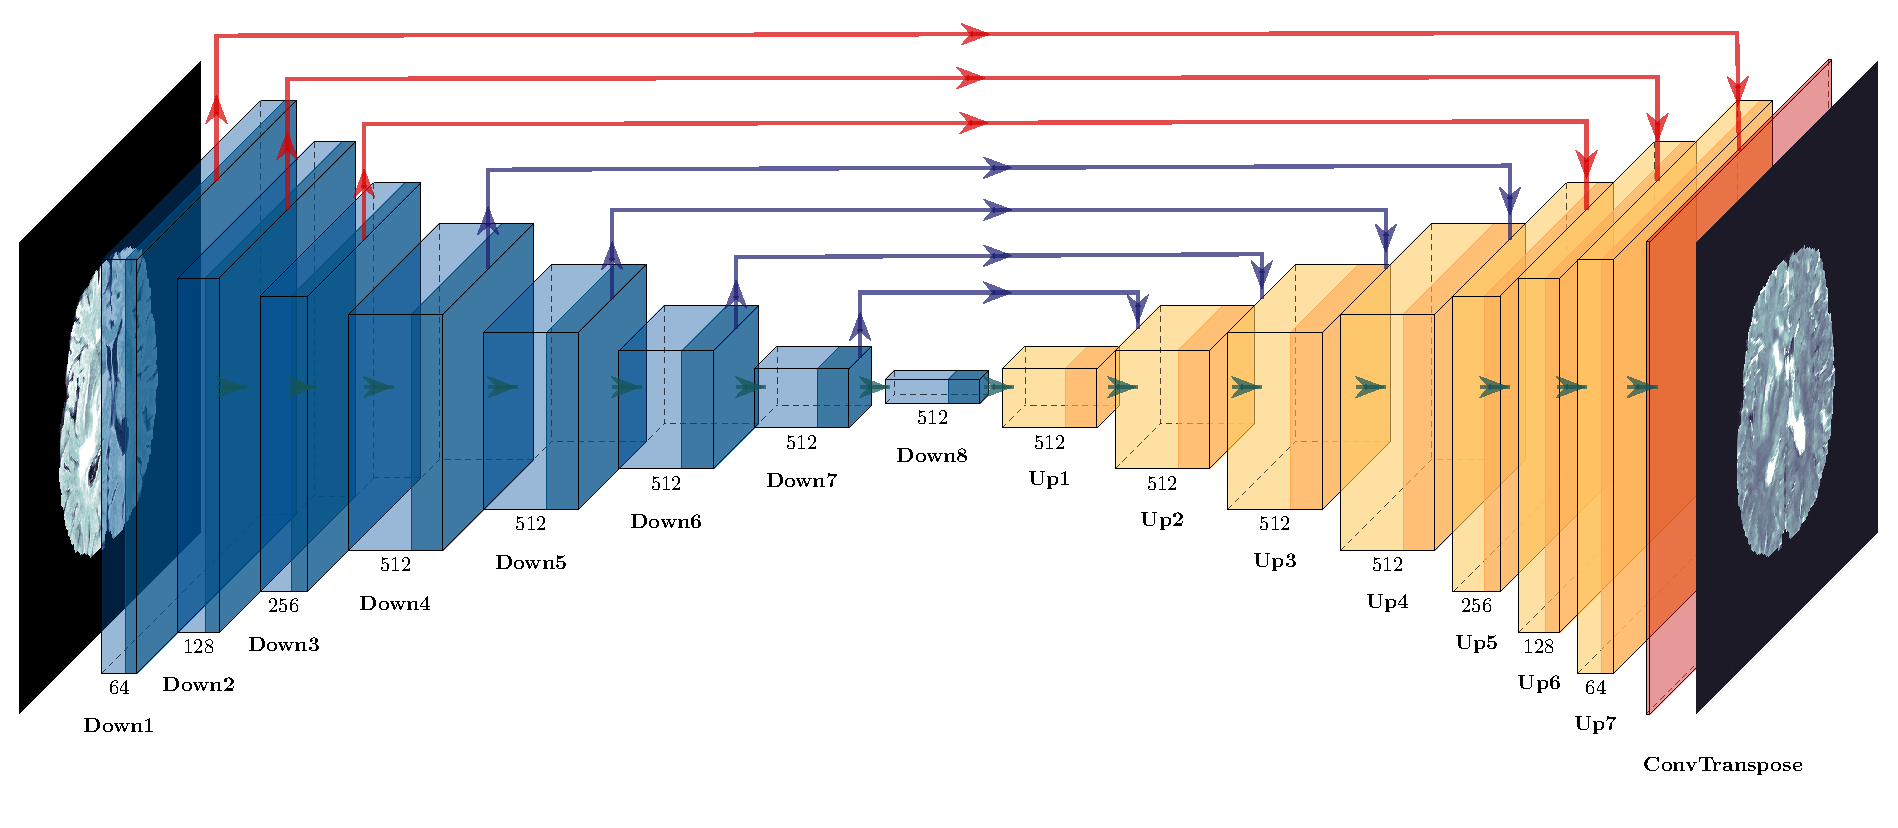
\includegraphics[height=0.266\textheight]{images/config_skips.pdf}
\caption[Configuration example in Skip Connections Analysis]{Example of network with the three outermost skip connections turned off/perturbed, corresponding to the configurations [1,1,1,1,0,0,0]/[AAAABBB].}
\label{fig:config_skips}
\end{figure}


%%%%%%%%%%%%%%%%  Channels off MI-p2p

\subsection{Channels Turned Off}
\label{subsec:skips_turned_off}
\begin{table}[H]
\centering
\fontsize{8.5}{16}\selectfont
\setlength{\tabcolsep}{4pt}
\begin{tabular}{l|c|c|c|c|c}
\toprule
\textbf{Skips off} & \textbf{MSE} & \textbf{PSNR} & \textbf{SSIM} & $\mathbf{MSE_{tumor}}$ & $\mathbf{PSNR_{tumor}}$\\
\hline

[1,1,1,1,1,1,1] & $\mathbf{0.0069\pm0.0049}$ & $\mathbf{22.8165\pm3.7317}$  & $\mathbf{0.7772\pm0.1094}$ & $\mathrm{0.0221\pm0.0375}$ & $\mathrm{19.0374\pm4.1582}$\\

[0,1,1,1,1,1,1] & $\mathrm{0.0071\pm0.0048}$ & $\mathrm{22.6609\pm3.7374}$  & $\mathrm{0.7718\pm0.1126}$ & $\mathbf{0.0209\pm0.0356}$ & $\mathbf{19.1225\pm4.0804}$\\

[0,0,1,1,1,1,1] & $\mathrm{0.0093\pm0.0053}$ & $\mathrm{21.3752\pm3.7214}$  & $\mathrm{0.7520\pm0.1163}$ & $\mathrm{0.0381\pm0.0251}$ & $\mathrm{14.8111\pm2.3423}$\\

[0,0,0,1,1,1,1] & $\mathrm{0.0103\pm0.0061}$ & $\mathrm{20.8808\pm3.6404}$  & $\mathrm{0.7217\pm0.1309}$ & $\mathrm{0.0374\pm0.0438}$ & $\mathrm{15.5332\pm3.1803}$\\

[0,0,0,0,1,1,1] & $\mathrm{0.0105\pm0.0059}$ & $\mathrm{20.8179\pm3.7360}$  & $\mathrm{0.7423\pm0.1175}$ & $\mathrm{0.0419\pm0.0235}$ & $\mathrm{14.3061\pm2.2416}$\\

[0,0,0,0,0,1,1] & $\mathrm{0.0147\pm0.0080}$ & $\mathrm{19.2806\pm3.4188}$  & $\mathrm{0.6610\pm0.1090}$ & $\mathrm{0.0779\pm0.0231}$ & $\mathrm{11.3254\pm1.6623}$\\

[0,0,0,0,0,0,1] & $\mathrm{0.0116\pm0.0060}$ & $\mathrm{20.1027\pm2.8014}$  & $\mathrm{0.5940\pm0.1035}$ & $\mathrm{0.0501\pm0.0212}$ & $\mathrm{13.3909\pm1.9644}$\\

[0,0,0,0,0,0,0] & $\mathrm{0.0987\pm0.0319}$ & $\mathrm{10.3797\pm1.8937}$  & $\mathrm{0.0202\pm0.0267}$ & $\mathrm{0.3230\pm0.1115}$ & $\mathrm{5.1401\pm1.4091}$\\
\hline
[1,1,1,1,1,1,1] & $\mathbf{0.0069\pm0.0049}$ & $\mathbf{22.8165\pm3.7317}$  & $\mathbf{0.7772\pm0.1094}$ & $\mathbf{0.0221\pm0.0375}$ & $\mathbf{19.0374\pm4.1582}$\\

[1,1,1,1,1,1,0] & $\mathrm{0.0105\pm0.0070}$ & $\mathrm{20.8009\pm3.3278}$  & $\mathrm{0.7434\pm0.1150}$ & $\mathrm{0.0332\pm0.0556}$ & $\mathrm{17.3071\pm4.3356}$\\

[1,1,1,1,1,0,0] & $\mathrm{0.0533\pm0.0256}$ & $\mathrm{13.4927\pm3.1335}$  & $\mathrm{0.3956\pm0.1498}$ & $\mathrm{0.1087\pm0.0973}$ & $\mathrm{10.8014\pm3.0530}$\\

[1,1,1,1,0,0,0] & $\mathrm{0.0846\pm0.0320}$ & $\mathrm{11.1146\pm1.9886}$  & $\mathrm{0.1106\pm0.0700}$ & $\mathrm{0.2253\pm0.1313}$ & $\mathrm{7.0131\pm2.0886}$\\

[1,1,1,0,0,0,0] & $\mathrm{0.0978\pm0.0336}$ & $\mathrm{10.4303\pm1.8611}$  & $\mathrm{0.0413\pm0.0491}$ & $\mathrm{0.3125\pm0.1390}$ & $\mathrm{5.3861\pm1.6662}$\\

[1,1,0,0,0,0,0] & $\mathrm{0.1050\pm0.0333}$ & $\mathrm{10.0808\pm1.7531}$  & $\mathrm{0.0134\pm0.0411}$ & $\mathrm{0.3362\pm0.1386}$ & $\mathrm{5.0176\pm1.5175}$\\

[1,0,0,0,0,0,0] & $\mathrm{0.0963\pm0.0315}$ & $\mathrm{10.4584\pm1.7412}$  & $\mathrm{0.0255\pm0.0419}$ & $\mathrm{0.3061\pm0.1227}$ & $\mathrm{5.4125\pm1.4862}$\\

[0,0,0,0,0,0,0] & $\mathrm{0.0987\pm0.0319}$ & $\mathrm{10.3797\pm1.8937}$  & $\mathrm{0.0202\pm0.0267}$ & $\mathrm{0.3230\pm0.1115}$ & $\mathrm{5.1401\pm1.4091}$\\
\midrule
\end{tabular}
\caption[Quantitative results from turning off the skips in MI-pix2pix]{Quantitative results from the Skip Connections Analysis on MI-P2P{$_{T_{2flair}}$}: skips are sequentially turned off.}
\label{tab:quantitative_channels_off_mip2p}
\end{table}

\begin{figure}[H]
\centering
\includegraphics[width=0.635\textheight]{images/skips_m2p.pdf}
\caption[Qualitative results from turning off the skips in MI-pix2pix]{Qualitative results from the Skip Connections Analysis on MI-P2P{$_{T_{2flair}}$}: skips are sequentially turned off. \textit{Prediction} corresponds to config.[1111111]}
\label{fig:qualitative_channels_off_mip2p}
\end{figure}

%\newpage
\subsection{Channels Perturbed}
\label{subsec:skips_perturbed}
%%%%%%%%%%%%%%%% Channels perturbed MI-p2p
\begin{table}[H]
\centering
\fontsize{8.5}{16}\selectfont
\setlength{\tabcolsep}{3.8pt}
\begin{tabular}{l|c|c|c|c|c}
\toprule
\textbf{Img.in Skips} & \textbf{MSE} & \textbf{PSNR} & \textbf{SSIM} & $\mathbf{MSE_{tumor}}$ & $\mathbf{PSNR_{tumor}}$\\
\hline

[AAAAAAA] & $\mathbf{0.0069\pm0.0049}$ & $\mathbf{22.8165\pm3.7317}$  & $\mathbf{0.7772\pm0.1094}$ & $\mathrm{0.0221\pm0.0375}$ & $\mathbf{19.0374\pm4.1582}$\\

[BAAAAAA] & $\mathrm{0.0071\pm0.0049}$ & $\mathrm{22.6889\pm3.7357}$  & $\mathrm{0.7753\pm0.1100}$ & $\mathbf{0.0213\pm0.0333}$ & $\mathrm{18.9774\pm4.0355}$\\

[BBAAAAA] & $\mathrm{0.0090\pm0.0054}$ & $\mathrm{21.5192\pm3.6746}$  & $\mathrm{0.7539\pm0.1145}$ & $\mathrm{0.0287\pm0.0330}$ & $\mathrm{16.7935\pm3.5473}$\\

[BBBAAAA] & $\mathrm{0.0113\pm0.0070}$ & $\mathrm{20.5749\pm3.6649}$  & $\mathrm{0.7329\pm0.1240}$ & $\mathrm{0.0429\pm0.0359}$ & $\mathrm{14.8824\pm3.4989}$\\

[BBBBAAA] & $\mathrm{0.0146\pm0.0085}$ & $\mathrm{19.2723\pm3.2735}$  & $\mathrm{0.7045\pm0.1187}$ & $\mathrm{0.0521\pm0.0425}$ & $\mathrm{14.0021\pm3.4752}$\\

[BBBBBAA] & $\mathrm{0.0372\pm0.0172}$ & $\mathrm{14.9083\pm2.6436}$  & $\mathrm{0.5024\pm0.1345}$ & $\mathrm{0.1032\pm0.0885}$ & $\mathrm{11.6955\pm4.6158}$\\

[BBBBBBA] & $\mathrm{0.0599\pm0.0282}$ & $\mathrm{12.9927\pm3.1396}$  & $\mathrm{0.4099\pm0.1852}$ & $\mathrm{0.1313\pm0.0917}$ & $\mathrm{9.9851\pm3.5551}$\\

[BBBBBBB] & $\mathrm{0.0921\pm0.0406}$ & $\mathrm{10.9644\pm2.5820}$  & $\mathrm{0.3257\pm0.1812}$ & $\mathrm{0.1871\pm0.1677}$ & $\mathrm{9.0777\pm4.4095}$\\
\hline
[AAAAAAA] & $\mathbf{0.0069\pm0.0049}$ & $\mathbf{22.8165\pm3.7317}$  & $\mathbf{0.7772\pm0.1094}$ & $\mathbf{0.0221\pm0.0375}$ & $\mathbf{19.0374\pm4.1582}$\\

[AAAAAAB] & $\mathrm{0.0122\pm0.0062}$ & $\mathrm{19.7162\pm2.3813}$  & $\mathrm{0.5947\pm0.1913}$ & $\mathrm{0.0272\pm0.0402}$ & $\mathrm{17.9227\pm4.1764}$\\

[AAAAABB] & $\mathrm{0.0318\pm0.0216}$ & $\mathrm{15.8378\pm2.7313}$  & $\mathrm{0.4635\pm0.1752}$ & $\mathrm{0.0584\pm0.0774}$ & $\mathrm{14.8665\pm4.7720}$\\

[AAAABBB] & $\mathrm{0.0734\pm0.0344}$ & $\mathrm{11.9599\pm2.5316}$  & $\mathrm{0.3481\pm0.1775}$ & $\mathrm{0.1300\pm0.1478}$ & $\mathrm{11.3327\pm5.0234}$\\

[AAABBBB] & $\mathrm{0.0820\pm0.0385}$ & $\mathrm{11.4885\pm2.5578}$  & $\mathrm{0.3384\pm0.1776}$ & $\mathrm{0.1800\pm0.1765}$ & $\mathrm{9.9064\pm5.2330}$\\

[AABBBBB] & $\mathrm{0.0863\pm0.0400}$ & $\mathrm{11.2936\pm2.6455}$  & $\mathrm{0.3300\pm0.1897}$ & $\mathrm{0.1705\pm0.1496}$ & $\mathrm{9.6293\pm4.6053}$\\

[ABBBBBB] & $\mathrm{0.0969\pm0.0378}$ & $\mathrm{10.6230\pm2.3366}$  & $\mathrm{0.3083\pm0.1755}$ & $\mathrm{0.1796\pm0.1473}$ & $\mathrm{9.1598\pm4.3589}$\\

[BBBBBBB] & $\mathrm{0.0921\pm0.0406}$ & $\mathrm{10.9644\pm2.5820}$  & $\mathrm{0.3257\pm0.1812}$ & $\mathrm{0.1871\pm0.1677}$ & $\mathrm{9.0777\pm4.4095}$\\
\midrule
\end{tabular}
\caption[Quantitative results from skips perturbation in MI-pix2pix]{Quantitative results from the Skip Connections Analysis on MI-P2P{$_{T_{2flair}}$}: skips are sequentially perturbed.}
\label{tab:quantitative_channels_perturbed_mip2p}
\end{table}

\begin{figure}[H]
\centering
\includegraphics[width=0.635\textheight]{images/a&b_mip2p.pdf}
\caption[Qualitative results from skips perturbation in MI-pix2pix]{Qualitative results from the Skip Connections Analysis on MI-P2P{$_{T_{2flair}}$}: skips are sequentially perturbed. \textit{Prediction} corresponds to config.[AAAAAAA]}
\label{fig:qualitative_channels_perturbed_mip2p}
\end{figure}


\section{Internal Connections Analysis}
\label{sec:internal_analysis}
In this section we present the analysis obtained by sequentially turning off the internal connections (or channels) of the generator network. 
The results are reported in Table \ref{tab:quantitative_internal_off_mip2p} and Figure \ref{fig:qualitative_internal_off_mip2p}, where, for example, a [1,1,1,1,1,0,0] configuration corresponds to switching off the 6th and 7th (and, as a consequence, the 9th and 10th, since the connections are switched in pairs) internal channels (Figure \ref{fig:config_internal}).


\begin{figure}[H]
\centering
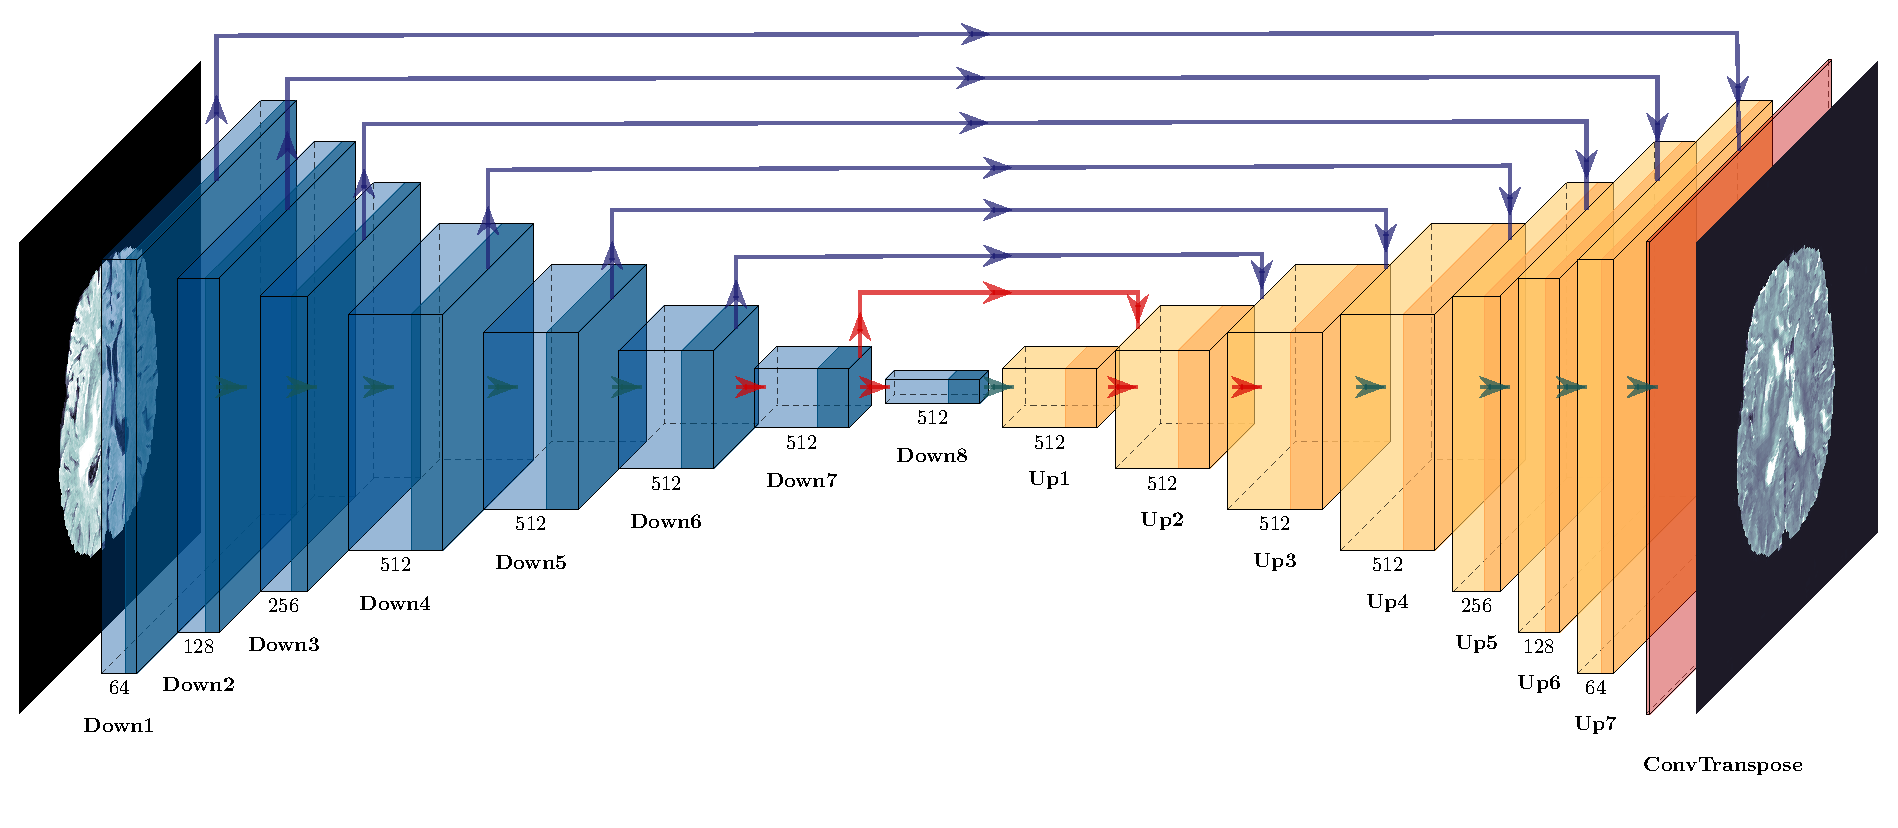
\includegraphics[height=0.266\textheight]{images/config_internal.pdf}
\caption[Configuration example in Internal Connections Analysis]{Example of network corresponding to the configuration [1,1,1,1,1,0,0] in the Internal Connections Analysis. In red the connections turned off.}
\label{fig:config_internal}
\end{figure}
\vspace{5mm}
It is worth to highlight that, even though this analysis focuses on the internal connections, when a pair of inner channels are off (except in the case of the 7th and 9th links), then also the entries of a skip connection are forced to 0, as it possible to observe in Figure \ref{fig:config_internal} where all the connections turned off are shown in red color.

%%%%%%%%%%%%%%%%  Internal connection analysis MI-p2p 
\begin{table}[H]
\centering
\fontsize{8.5}{16}\selectfont
\setlength{\tabcolsep}{4pt}
\begin{tabular}{c|c|c|c|c|c}
\toprule
\textbf{Internal off} & \textbf{MSE} & \textbf{PSNR} & \textbf{SSIM} & $\mathbf{MSE_{tumor}}$ & $\mathbf{PSNR_{tumor}}$\\
\hline

[1,1,1,1,1,1,1] & $\mathbf{0.0069\pm0.0049}$ & $\mathbf{22.8165\pm3.7317}$  & $\mathbf{0.7772\pm0.1094}$ & $\mathbf{0.0221\pm0.0375}$ & $\mathbf{19.0374\pm4.1582}$\\

[0,1,1,1,1,1,1] & $\mathrm{0.0103\pm0.0058}$ & $\mathrm{20.8939\pm3.7816}$  & $\mathrm{0.7062\pm0.1355}$ & $\mathrm{0.0406\pm0.0173}$ & $\mathrm{14.3578\pm2.0877}$\\

... & ... & ... & ... & ... & ... \\

[0,0,0,0,0,0,0] & $\mathrm{0.0103\pm0.0058}$ & $\mathrm{20.8939\pm3.7816}$  & $\mathrm{0.7062\pm0.1355}$ & $\mathrm{0.0406\pm0.0173}$ & $\mathrm{14.3578\pm2.0877}$\\
\hline
[1,1,1,1,1,1,1] & $\mathbf{0.0069\pm0.0049}$ & $\mathrm{22.8165\pm3.7317}$  & $\mathrm{0.7772\pm0.1094}$ & $\mathrm{0.0221\pm0.0375}$ & $\mathbf{19.0374\pm4.1582}$\\

[1,1,1,1,1,1,0] & $\mathbf{0.0069\pm0.0049}$ & $\mathbf{22.8750\pm3.7301}$  & $\mathbf{0.7794\pm0.1084}$ & $\mathbf{0.0218\pm0.0346}$ & $\mathrm{18.9272\pm4.0549}$\\

[1,1,1,1,1,0,0] & $\mathrm{0.0077\pm0.0048}$ & $\mathrm{22.2194\pm3.6022}$  & $\mathrm{0.7579\pm0.1165}$ & $\mathrm{0.0229\pm0.0384}$ & $\mathrm{18.4526\pm3.8248}$\\

[1,1,1,1,0,0,0] & $\mathrm{0.0095\pm0.0054}$ & $\mathrm{21.2806\pm3.7368}$  & $\mathrm{0.7505\pm0.1164}$ & $\mathrm{0.0393\pm0.0253}$ & $\mathrm{14.6543\pm2.3238}$\\

[1,1,1,0,0,0,0] & $\mathrm{0.0104\pm0.0062}$ & $\mathrm{20.8601\pm3.6599}$  & $\mathrm{0.7192\pm0.1326}$ & $\mathrm{0.0400\pm0.0454}$ & $\mathrm{15.1987\pm3.1458}$\\

[1,1,0,0,0,0,0] & $\mathrm{0.0108\pm0.0059}$ & $\mathrm{20.6812\pm3.7336}$  & $\mathrm{0.7403\pm0.1178}$ & $\mathrm{0.0444\pm0.0259}$ & $\mathrm{14.0582\pm2.2371}$\\

[1,0,0,0,0,0,0] & $\mathrm{0.0162\pm0.0086}$ & $\mathrm{18.8502\pm3.5119}$  & $\mathrm{0.6641\pm0.1233}$ & $\mathrm{0.0845\pm0.0249}$ & $\mathrm{10.9653\pm1.7048}$\\

[0,0,0,0,0,0,0] & $\mathrm{0.0103\pm0.0058}$ & $\mathrm{20.8939\pm3.7816}$  & $\mathrm{0.7062\pm0.1355}$ & $\mathrm{0.0406\pm0.0173}$ & $\mathrm{14.3578\pm2.0877}$\\
\midrule
\end{tabular}
\caption[Quantitative results from internal connections off in MI-pix2pix]{Quantitative results from the Internal Connections Analysis on MI-P2P{$_{T_{2flair}}$}: channels are sequentially turned off.}
\label{tab:quantitative_internal_off_mip2p}
\end{table}

\begin{figure}[H]
\includegraphics[width=0.635\textheight]{images/internal_mip2p.pdf}
\caption[Qualitative results from internal connections off in MI-pix2pix]{Qualitative results from the Internal Connections Analysis on MI-P2P{$_{T_{2flair}}$}: channels are sequentially turned off. \textit{Prediction} corresponds to config.[1111111]}


\centering
\label{fig:qualitative_internal_off_mip2p}
\end{figure}
\newpage
\section{Experiments Discussion}
\label{sec:experiments_discussion}
While in Subsection \ref{subsec:metrics_discussion} we demonstrated that the input received by our models isn't just outputted but it is elaborated, allowing to produce a completely new synthesized image, in Sections \ref{sec:skip_analysis} and \ref{sec:internal_analysis} we investigated about which connections, in a generator network, are used the most in this processing: in this section we discuss the results obtained from the experiments presented in the previous sections, eventually referring to the additional results reported in \autoref{cha:first_appendix}.

\vspace{5mm}
Table \ref{tab:quantitative_internal_off_mip2p}, reporting the quantitative results from the Internal Connection Analysis, shows that all the configurations with the the first (and the last, since they are turned off in pairs) internal channels off reach the exactly same performances in the evaluation metrics. This is due to the fact that all the entries of the connection between the last and the second-last layers are set to 0 and so the information coming from the input is sent to the output only through the outermost skip connection.

\vspace{5mm}
Looking at the values from Table \ref{tab:quantitative_internal_off_mip2p} it is possible to appreciate how the values in the performances don't deteriorate too much compared to the configuration with all the channels on. This is a first indicator about the importance of the skips connections in the generator networks: with all the internal connections off and with all the skips off with the exception of the outermost, the network is able to still obtain satisfiable results, with a worsening in the performance of 49\% in MSE, 8\% in PSNR, 9\% in SSIM, 84\% in $MSE_{tumor}$ and 25\% in $PSNR_{tumor}$. 

\vspace{5mm}
Observing Tables \ref{tab:quantitative_channels_off_mip2p} and \ref{tab:quantitative_channels_perturbed_mip2p} from the Skip Connection Analysis, we can confirm the major role played by the outermost skip connection in the generative process: when all the skips values are forced to 0 and the information passes only through internal connections, the network performs worse, compared to the [1111111] configuration, by a significant degradation of 1330\% in MSE, 55\% in PSNR, 97\% in SSIM, 1362\% in $MSE_{tumor}$ and 73\% in $PSNR_{tumor}$ (Figure \ref{fig:barplot_1}).

\begin{figure}
\centering
\includegraphics[width=0.635\textheight]{images/barplot_1.pdf}
\caption[Percentual degradation in the performances of MI-pix2pix]{Percentual degradation observed in the performances of MI-pix2pix, with respect to the configuration with all the connections, skips and internal, ON (Config. [1111111]).}
\label{fig:barplot_1}
\end{figure}


This degradation in the performances can be easily appreciated also by a visual comparison of the qualitative results shown in Figure \ref{fig:qualitative_channels_off_mip2p} and it reinforces the hypothesis that these connections are crucial for a generative model since they allow to recover the information lost in the contracting path through the many downsampling blocks.

\vspace{5mm}
The outermost skip is for sure the connection that brings the most significant source of information to the output image but in general, looking both at Figure \ref{fig:qualitative_channels_off_mip2p} and Table \ref{tab:quantitative_channels_off_mip2p}, we can observe how the scores obtained from the metrics drop to low values more rapidly by switching off the outer connections than switching first the inner ones, due to the fact the most external skips are crucial for a Generative Adversarial network.

\vspace{5mm}
The results we obtained in the second part (skips perturbed, Subsection \ref{subsec:skips_perturbed}) of the Skip Connections Analysis are consistent with what was observed in the first one (skips off, Subsection \ref{subsec:skips_turned_off}) and show a similar behaviour in the degradation of the performances. 
The qualitative results, instead, show even better what we said about the most external links: Figure \ref{fig:qualitative_channels_perturbed_mip2p} illustrates how the appearance belonging to the image $A$ is completely almost compromised after perturbing the generator with the replacement, in two outermost skip connections, of the content belonging to $A$ with the one produced by another network that takes as input $B$.

\vspace{5mm}
Further experiments on MI-GAN and pix2pix, that can be found in Appendix \ref{cha:first_appendix}, show that the unimodal model, compared to two multi-modal networks, seems to have more balance in the gap between the contributions of the skip connections to the generated image: the outermost skip connections remain the most significant for the generative process but to a lesser extent with respect to what we observed with the multi-input generator. 

\begin{figure}
\centering
\includegraphics[width=0.635\textheight]{images/barplot_2.pdf}
\caption[Percentual degradation in the performances of different models]{Percentual degradation observed in the performances of the different models when all the internal channels are turned off (and so every skip connections is off, except for the outermost one), with respect to the configuration with all the connections, skips and internal, ON (Config. [1111111]).}
\label{fig:barplot_2}
\end{figure}

This can be visually appreciated by a comparison between Figures \ref{fig:qualitative_channels_off_p2p} and \ref{fig:qualitative_channels_off_mip2p} but also by the quantitative results from the analysis on the internal connections, with pix2pix that, switching off all the connections except for the last skip channel, deteriorates more (238\% in MSE, 25\% in PSNR, 21\% in SSIM) than MI-pix2pix (49\% in MSE, 8\% in PSNR, 9\% in SSIM) and MI-GAN (72\% in MSE, 11\% in PSNR, 15\% in SSIM) (Figure \ref{fig:barplot_2}).


\section{Summary}
\label{sec:6th_section_summary}
In this chapter we presented the experiments conducted in order to investigate about which are the connections used the most during the generative process of the models we trained.

Then we reported and evaluated both the quantitative and the qualitative results reached with our tests, discussing the observed behaviour of the generator network and showing the insights provided by the Skip Connections Analysis and by the Internal Connections Analysis: the experiments performed led us to the conclusion that skip connections (in particular the outermost skip connections) have a crucial role in the generative process and by turning off or perturbing these channels, a significant degradation in the performances of the network is observed.

\vspace{5mm}
In the next chapter, we provide more general considerations on our work and we present the open problems as well as the possible future works.
\chapter{Conclusions and Future Work}
\label{cha:7th_chapter}
In this chapter we make our final considerations about this work: first by reporting our conclusions in Section \ref{sec:conclusions}, then by discussing the open problems and the possible applications in which the framework presented could be used (Section \ref{sec:future_work}).

\section{Conclusions}
\label{sec:conclusions}


In Chapter \ref{cha:5th_chapter} we showed the results obtained by using Generative Adversarial Networks to synthesize missing modalities after training the models with thousands of brain MRI slices: the generated images are highly accurate and realistic, compared to sequences belonging to the dataset, and in many cases it is objectively difficult to distinguish between true and fake images.

Because of this we are overall satisfied by the generation quality of the images and by the achieved results (measured by the different evaluation metrics implemented) that are extremely encouraging for future develops and demonstrate the applicability of \ac{GAN}s in neuroimaging. 
In Chapter \ref{cha:6th_chapter}, then, we also showed, through various experiments on the trained models, the effectiveness of the skip connections, crucial to recover spatial information otherwise lost in the downsampling part of the Generator network.

We found cases where the image wasn't a realistic copy of the ground truth, but not due to some bad implementation choices but because the missing modality generated is originally obtained using a contrast agent and so it has a highly specific information difficult to reproduce and not present in any other sequence. 

However, the models implemented are far from being perfect with the generated sequences that in some cases contained blurred artifacts or low-level details not perfectly defined.

\vspace{5mm}
In general, the multi-modal models tested have proved to be better than unimodal \ac{GAN}s (except in the case in which target and input images present highly similar characteristics), due to the fact that they can exploit the correlation between available sequences, allowing us to reduce the order of magnitude of required models (from 12 single-input single-output to 4 multi-input single-output). The results obtained in this work demonstrate the possibility of using successfully this generative framework as a part of a bigger pipeline that can generate and then segment the synthesized missing modality, giving to the doctors an additional aid for the diagnosis of brain tumors.
\section{Future Work}
\label{sec:future_work}
In this section we describe the open problems encountered during the work and we propose different solutions to improve the system designed and to make possible, in the future, its employment in medical imaging.

\subsection{Open Problems}
\label{subsec:open_problems}
%\vspace{6mm} 
\noindent\textbf{Data Availability}

\vspace{2mm}
\noindent The amount of data available is crucial for any deep learning setting and the scarcity of annotated samples represents a huge problem, especially, for all the systems working in the medical imaging domain. In our case, the first problem we had to deal with, working with a medical dataset, was that BRATS2015, built for a segmentation challenge, was composed by two parts: one intended for the training and one for the testing, without annotated and segmented samples. So we could use only the first set of data, since we needed ground truths to evaluate the tumor area and to assess the quality of the segmentation obtained with the \ac{GAN} predictions.

The second problem we faced was that our reduced dataset is composed by 35.072 slices per modality (with 28.160 used for the training) but all these images belong to the volumes of 274 subjects (training set reduced to 219 patients), so the samples in the dataset are not independent and most of these slices contain very similar information.

\vspace{6mm} 
\noindent\textbf{Evaluation Metrics}

\vspace{2mm}
\noindent 
Another common and open problem is the one related to evaluation of the results produced by a Generative Adversarial Network: many works, and so did we, adopt metrics such as PSNR and SSIM to quantitatively evaluate the generated image but the problem is that these measures don't correspond to the visual quality of the image. 

GAN evaluation is not a settled issue yet and researchers suggest to validate the quality of the prediction by using segmentation models, as we did in Subsection \ref{subsec:segmentation_results}, or, even better, to recruit domain experts that could evaluate the results generated by the network: this, unfortunately, is not always accomplishable since it is expensive and time-consuming \cite{Yi_2019}.

\subsection{Possible Applications and Future Develops}
\label{sec:possible_applications}
\vspace{6mm} 
\noindent\textbf{Improving the MSE and PSNR implemented }

\vspace{2mm}
\noindent 
In our work we calculated the MSE and PSNR over the whole image, considering the pixels belonging to the brain as well as the ones with zero value. The reasoning behind is that the \ac{GAN} learns to generate also the black pixels so it is not wrong to measure the similarity and the error over the overall area. 

An alternative approach could be to modify the MSE and the PSNR implementation considering only the pixels with value different from zero and the ones not belonging to the tumor: by doing this it would be possible to understand, through a direct comparison, if the generation quality in the malignant area is higher/equal/lower with respect to the rest of the brain.

\vspace{6mm} 
\noindent\textbf{Tweaking the model}

\vspace{2mm}
\noindent 
In our case we used the hyperparameters values defined by \cite{pix2pix} and \cite{migan}, since we couldn't find any improvements over the defined values. We believe that networks capabilities can be increased by tweaking the model to find the optimal parameters. 


\vspace{6mm} 
\noindent\textbf{Variable number of inputs to the multi-modal model}

\vspace{2mm}
\noindent 
One way to improve the multi-modal networks developed would be to train them to synthesize one image in the presence of a variable numbers of input sequences (while in our case, we need to use the slices from all the three different modalities, in order to be able to synthesize the missing image).

\vspace{6mm} 
\noindent\textbf{Multi-input Multi-output model}

\vspace{2mm}
\noindent 
It would be interesting, then, to study possible improvements in the direction of multi-input multi-output models, where some researchers have already started to experiment with, such as Sharma et al. with their proposed MM-GAN \cite{migan}.
\newpage
\vspace{6mm} 
\noindent\textbf{Possible Applications}

\vspace{2mm}
\noindent The most obvious application of our work, as discussed in previous sections, would be to use the developed network as a part of a bigger pipeline of downstream analysis, such as segmentation, in order to improve the daily workflow of the radiologists. Some segmentation models indeed depend on the implicit assumption that all the input sequences are available: because of this, if some modalities, due to various reasons, are missing, then a generative adversarial network trained on brain \ac{MRI} would be very useful to synthesize the images needed.

This generative framework has many possible applications in different medical settings and lots of studies have been focusing on how to get the most from these networks. For instance, \ac{GAN}s would be very useful in \ac{MRI} image restoration where artifacts due to errors/motions during the scan can be removed, avoiding to repeat the exams multiple times. However, it's important to underline that, as Yi et al. suggests in \cite{Yi_2019}, \ac{GAN}-based methods are still far from being adopted clinically: this field is still in its infancy and a lot of work has to be done yet.

% Appendici
\renewcommand{\chaptermark}[1]{\markboth{\appendixname\ \thechapter.\ #1}{}} % modifica l'intestazione con il nome/lettera dell'appendice
\fancyhead[LE,RO]{\leftmark}


% Acronimi
\chapter*{Acronyms}
\label{cha:acronyms}
\addcontentsline{toc}{chapter}{Acronyms}

\begin{acronym}[\qquad \qquad \qquad \quad]
\acro{AI}{Artificial Intelligence}
\acro{cGAN}{conditional GAN}
\acro{CNN}{Convolutional Neural Network}
\acro{CNNs}{Convolutional Neural Networks}
\acro{CSF}{Cerebrospinal fluid}
\acro{CT}{Computerized Tomography}
\acro{DL}{Deep Learning}
\acro{GAN}{Generative Adversarial Network}
\acro{GANs}{Generative Adversarial Networks}
\acro{GPU}{Graphics processing unit}
\acro{GPUs}{Graphics processing units}
\acro{MR}{Magnetic Resonance}
\acro{MRA}{Magnetic Resonance Angiohraphy}
\acro{MRI}{Magnetic Resonance Imaging}
\acro{NN}{Neural Network}
\acro{PET}{Positron Emission Tomography}

\end{acronym}


% modifica intestazione della bibliografia
\fancyhead[LE,RO]{\nouppercase{\leftmark}} % cancella il tutto maiuscolo


% bibliografia
%\input{chapters/bibliography}
% because the file is called 'bibliography.tex'

\bibliographystyle{IEEEtran}
\bibliography{chapters/bibliography}
% to remove Bibliography from list of contents, remove the relative package (tocbibind).
\appendix % trasforma i numeri in lettere per fare l'appendice
\chapter{Appendix: Further Results from Connections Analysis}
\label{cha:first_appendix}

In this Appendix we report additional (quantitative and qualitative) results obtained from the following experiments (in the same order as they are presented): 

\begin{itemize}
\item Skip Connections Analysis on P2P$(T_{2 \rightarrow 2flair})$ and MI-GAN{$_{T_{2flair}}$} with channels turned off.
\item Skip Connections Analysis on P2P$(T_{2 \rightarrow 2flair})$ and MI-GAN{$_{T_{2flair}}$} with channels perturbed.
\item Internal Connections Analysis on P2P$(T_{2 \rightarrow 2flair})$ and MI-GAN{$_{T_{2flair}}$} with channels turned off.
\end{itemize}

\noindent In the following tables, values in boldface represent best performance values. The reported values are mean $\pm$ std.

%%%%%%%%%%%%%%%%  Channels turned off p2p 

\newpage
\begin{table}[H]
\centering
\caption[Quantitative results from turning off the skips in pix2pix]{Quantitative results from the Skip Connections Analysis on P2P$(T_{2 \rightarrow 2flair})$: skips are sequentially turned off.}
\fontsize{8.5}{16}\selectfont
\setlength{\tabcolsep}{4pt}
\begin{tabular}{l|c|c|c|c|c}
\toprule
\textbf{Skips off} & \textbf{MSE} & \textbf{PSNR} & \textbf{SSIM} & $\mathbf{MSE_{tumor}}$ & $\mathbf{PSNR_{tumor}}$\\
\hline

[1,1,1,1,1,1,1] & $\mathrm{0.0090\pm0.0065}$ & $\mathbf{21.5895\pm3.4831}$  & $\mathbf{0.7518\pm0.1211}$ & $\mathbf{0.0390\pm0.0463}$ & $\mathrm{15.9946\pm4.0459}$\\

[0,1,1,1,1,1,1] & $\mathbf{0.0090\pm0.0062}$ & $\mathrm{21.5423\pm3.3860}$  & $\mathrm{0.7515\pm0.1204}$ & $\mathrm{0.0391\pm0.0473}$ & $\mathbf{16.0047\pm4.0874}$\\

[0,0,1,1,1,1,1] & $\mathrm{0.0099\pm0.0068}$ & $\mathrm{21.1858\pm3.6324}$  & $\mathrm{0.7436\pm0.1268}$ & $\mathrm{0.0464\pm0.0422}$ & $\mathrm{14.6891\pm3.6658}$\\

[0,0,0,1,1,1,1] & $\mathrm{0.0139\pm0.0086}$ & $\mathrm{19.7127\pm3.7077}$  & $\mathrm{0.7069\pm0.1398}$ & $\mathrm{0.0792\pm0.0634}$ & $\mathrm{12.0341\pm3.1018}$\\

[0,0,0,0,1,1,1] & $\mathrm{0.0147\pm0.0086}$ & $\mathrm{19.4145\pm3.5775}$  & $\mathrm{0.6591\pm0.1253}$ & $\mathrm{0.0845\pm0.0370}$ & $\mathrm{11.1662\pm2.0567}$\\

[0,0,0,0,0,1,1] & $\mathrm{0.0160\pm0.0104}$ & $\mathrm{19.0200\pm3.4598}$  & $\mathrm{0.6440\pm0.1113}$ & $\mathrm{0.0440\pm0.0255}$ & $\mathrm{14.2132\pm2.3999}$\\

[0,0,0,0,0,0,1] & $\mathrm{0.0494\pm0.0285}$ & $\mathrm{13.8789\pm2.8530}$  & $\mathrm{0.1962\pm0.0692}$ & $\mathrm{0.1423\pm0.0613}$ & $\mathrm{8.8606\pm1.9105}$\\

[0,0,0,0,0,0,0] & $\mathrm{0.1229\pm0.0630}$ & $\mathrm{9.7545\pm2.5459}$  & $\mathrm{-0.0072\pm0.0352}$ & $\mathrm{0.3883\pm0.1420}$ & $\mathrm{4.3978\pm1.6224}$\\
\hline
[1,1,1,1,1,1,1] & $\mathbf{0.0090\pm0.0065}$ & $\mathbf{21.5895\pm3.4831}$  & $\mathbf{0.7518\pm0.1211}$ & $\mathbf{0.0390\pm0.0463}$ & $\mathbf{15.9946\pm4.0459}$\\

[1,1,1,1,1,1,0] & $\mathrm{0.0155\pm0.0085}$ & $\mathrm{18.8593\pm2.9462}$  & $\mathrm{0.6954\pm0.1149}$ & $\mathrm{0.0682\pm0.0726}$ & $\mathrm{13.1789\pm3.6046}$\\

[1,1,1,1,1,0,0] & $\mathrm{0.0431\pm0.0194}$ & $\mathrm{14.1364\pm2.1434}$  & $\mathrm{0.3764\pm0.1560}$ & $\mathrm{0.1378\pm0.1250}$ & $\mathrm{9.9799\pm3.6409}$\\

[1,1,1,1,0,0,0] & $\mathrm{0.0380\pm0.0187}$ & $\mathrm{14.7498\pm2.2690}$  & $\mathrm{0.3761\pm0.1271}$ & $\mathrm{0.0915\pm0.0927}$ & $\mathrm{11.9744\pm3.7576}$\\

[1,1,1,0,0,0,0] & $\mathrm{0.0789\pm0.0286}$ & $\mathrm{11.3898\pm1.9330}$  & $\mathrm{0.1219\pm0.0759}$ & $\mathrm{0.1838\pm0.1397}$ & $\mathrm{8.3547\pm3.0633}$\\

[1,1,0,0,0,0,0] & $\mathrm{0.0982\pm0.0319}$ & $\mathrm{10.3641\pm1.7303}$  & $\mathrm{0.0404\pm0.0606}$ & $\mathrm{0.2792\pm0.1765}$ & $\mathrm{6.1384\pm2.1748}$\\

[1,0,0,0,0,0,0] & $\mathrm{0.0929\pm0.0335}$ & $\mathrm{10.5920\pm1.5696}$  & $\mathrm{0.0489\pm0.0610}$ & $\mathrm{0.2497\pm0.1228}$ & $\mathrm{6.4492\pm1.8823}$\\

[0,0,0,0,0,0,0] & $\mathrm{0.1229\pm0.0630}$ & $\mathrm{9.7545\pm2.5459}$  & $\mathrm{-0.0072\pm0.0352}$ & $\mathrm{0.3883\pm0.1420}$ & $\mathrm{4.3978\pm1.6224}$\\
\midrule
\end{tabular}
\label{tab:quantitative_channels_off_p2p}
\end{table}

\begin{figure}[H]
\centering
\caption[Qualitative results from turning off the skips in pix2pix]{Qualitative results from the Skip Connections Analysis on P2P$(T_{2 \rightarrow 2flair})$: skips are sequentially turned off. \textit{Prediction} corresponds to config.[1111111]}
\includegraphics[width=0.635\textheight]{images/skips_p2p.pdf}

\label{fig:qualitative_channels_off_p2p}
\end{figure}

%%%%%%%%%%%%%%%%  Channels turned off MI-GAN 

\newpage

\begin{table}[H]
\centering
\caption[Quantitative results from turning off the skips in MI-GAN]{Quantitative results from the Skip Connections Analysis on MI-GAN{$_{T_{2flair}}$}: skips are sequentially turned off.}
\fontsize{8.5}{16}\selectfont
\setlength{\tabcolsep}{4pt}
\begin{tabular}{l|c|c|c|c|c}
\toprule
\textbf{Skips off} & \textbf{MSE} & \textbf{PSNR} & \textbf{SSIM} & $\mathbf{MSE_{tumor}}$ & $\mathbf{PSNR_{tumor}}$\\
%\begin{tabular}[l]{@{}l@{}}\textbf{Channels}\\ %\textbf{activation}\end{tabular} & \textbf{MSE} & \textbf{PSNR} & %\textbf{SSIM} & $\mathbf{MSE_{tumor}}$ & $\mathbf{PSNR_{tumor}}$\\
\hline

[1,1,1,1,1,1,1] & $\mathbf{0.0072\pm0.0050}$ & $\mathbf{22.5524\pm3.5655}$  & $\mathbf{0.7610\pm0.1175}$ & $\mathbf{0.0258\pm0.0285}$ & $\mathbf{17.4694\pm3.6137}$\\

[0,1,1,1,1,1,1] & $\mathrm{0.0081\pm0.0051}$ & $\mathrm{21.9370\pm3.3825}$  & $\mathrm{0.7439\pm0.1210}$ & $\mathrm{0.0277\pm0.0305}$ & $\mathrm{17.1080\pm3.5332}$\\

[0,0,1,1,1,1,1] & $\mathrm{0.0100\pm0.0065}$ & $\mathrm{21.0970\pm3.6387}$  & $\mathrm{0.7375\pm0.1233}$ & $\mathrm{0.0346\pm0.0165}$ & $\mathrm{15.1511\pm2.3996}$\\

[0,0,0,1,1,1,1] & $\mathrm{0.0138\pm0.0069}$ & $\mathrm{19.3884\pm3.1246}$  & $\mathrm{0.6734\pm0.1387}$ & $\mathrm{0.0496\pm0.0448}$ & $\mathrm{14.2094\pm3.3076}$\\

[0,0,0,0,1,1,1] & $\mathrm{0.0109\pm0.0074}$ & $\mathrm{20.8007\pm3.7417}$  & $\mathrm{0.7324\pm0.1244}$ & $\mathrm{0.0331\pm0.0157}$ & $\mathrm{15.3792\pm2.5432}$\\

[0,0,0,0,0,1,1] & $\mathrm{0.0125\pm0.0072}$ & $\mathrm{19.8870\pm2.9944}$  & $\mathrm{0.5906\pm0.0975}$ & $\mathrm{0.0389\pm0.0172}$ & $\mathrm{14.5971\pm2.2820}$\\

[0,0,0,0,0,0,1] & $\mathrm{0.0273\pm0.0109}$ & $\mathrm{16.0275\pm1.8843}$  & $\mathrm{0.1886\pm0.0422}$ & $\mathrm{0.1012\pm0.0370}$ & $\mathrm{10.2183\pm1.5814}$\\

[0,0,0,0,0,0,0] & $\mathrm{0.1294\pm0.0434}$ & $\mathrm{9.2003\pm1.8129}$  & $\mathrm{0.0039\pm0.0061}$ & $\mathrm{0.3872\pm0.1252}$ & $\mathrm{4.3380\pm1.3904}$\\
\hline
[1,1,1,1,1,1,1] & $\mathbf{0.0072\pm0.0050}$ & $\mathbf{22.5524\pm3.5655}$  & $\mathbf{0.7610\pm0.1175}$ & $\mathbf{0.0258\pm0.0285}$ & $\mathbf{17.4694\pm3.6137}$\\

[1,1,1,1,1,1,0] & $\mathrm{0.0077\pm0.0051}$ & $\mathrm{22.1638\pm3.3988}$  & $\mathrm{0.7566\pm0.1170}$ & $\mathrm{0.0301\pm0.0335}$ & $\mathrm{16.7878\pm3.5362}$\\

[1,1,1,1,1,0,0] & $\mathrm{0.0424\pm0.0213}$ & $\mathrm{14.5579\pm3.3720}$  & $\mathrm{0.4903\pm0.1508}$ & $\mathrm{0.1013\pm0.0885}$ & $\mathrm{11.2495\pm3.3876}$\\

[1,1,1,1,0,0,0] & $\mathrm{0.0886\pm0.0293}$ & $\mathrm{10.8085\pm1.6658}$  & $\mathrm{0.0805\pm0.0646}$ & $\mathrm{0.2480\pm0.1308}$ & $\mathrm{6.4845\pm1.8742}$\\

[1,1,1,0,0,0,0] & $\mathrm{0.1157\pm0.0352}$ & $\mathrm{9.6557\pm1.8085}$  & $\mathrm{-0.0183\pm0.0419}$ & $\mathrm{0.3456\pm0.1628}$ & $\mathrm{4.9657\pm1.6754}$\\

[1,1,0,0,0,0,0] & $\mathrm{0.1266\pm0.0397}$ & $\mathrm{9.2731\pm1.8176}$  & $\mathrm{-0.0275\pm0.0328}$ & $\mathrm{0.3742\pm0.1696}$ & $\mathrm{4.6018\pm1.6302}$\\

[1,0,0,0,0,0,0] & $\mathrm{0.1176\pm0.0398}$ & $\mathrm{9.6350\pm1.9156}$  & $\mathrm{0.0060\pm0.0162}$ & $\mathrm{0.3659\pm0.1532}$ & $\mathrm{4.6860\pm1.6421}$\\

[0,0,0,0,0,0,0] & $\mathrm{0.1294\pm0.0434}$ & $\mathrm{9.2003\pm1.8129}$  & $\mathrm{0.0039\pm0.0061}$ & $\mathrm{0.3872\pm0.1252}$ & $\mathrm{4.3380\pm1.3904}$\\
\midrule
\end{tabular}
\label{tab:quantitative_channels_off_migan}
\end{table}

\begin{figure}[H]
\centering
\caption[Qualitative results from turning off the skips in MI-GAN]{Qualitative results from the Skip Connections Analysis on MI-GAN{$_{T_{2flair}}$}: skips are sequentially turned off. \textit{Prediction} corresponds to config.[1111111]}
\includegraphics[width=0.635\textheight]{images/skips_migan.pdf}
\label{fig:qualitative_channels_off_migan}
\end{figure}

%%%%%%%%%%%%%%%%  Channels perturbed p2p 

\begin{table}[H]
\centering
\caption[Quantitative results from skips perturbation in pix2pix]{Quantitative results from the Skip Connections Analysis on P2P$(T_{2 \rightarrow 2flair})$: skips are sequentially perturbed.}
\fontsize{8.5}{16}\selectfont
\setlength{\tabcolsep}{3.8pt}
\begin{tabular}{l|c|c|c|c|c}
\toprule
\textbf{Img.in Skips} & \textbf{MSE} & \textbf{PSNR} & \textbf{SSIM} & $\mathbf{MSE_{tumor}}$ & $\mathbf{PSNR_{tumor}}$\\
\hline

[AAAAAAA] & $\mathbf{0.0090\pm0.0065}$ & $\mathbf{21.5895\pm3.4831}$  & $\mathbf{0.7518\pm0.1211}$ & $\mathbf{0.0390\pm0.0463}$ & $\mathbf{15.9946\pm4.0459}$\\

[BAAAAAA] & $\mathrm{0.0091\pm0.0064}$ & $\mathrm{21.5235\pm3.4479}$  & $\mathrm{0.7513\pm0.1210}$ & $\mathrm{0.0396\pm0.0460}$ & $\mathrm{15.8619\pm3.9731}$\\

[BBAAAAA] & $\mathrm{0.0104\pm0.0069}$ & $\mathrm{20.8839\pm3.4477}$  & $\mathrm{0.7383\pm0.1270}$ & $\mathrm{0.0505\pm0.0435}$ & $\mathrm{14.2265\pm3.4858}$\\

[BBBAAAA] & $\mathrm{0.0158\pm0.0087}$ & $\mathrm{18.8661\pm3.0820}$  & $\mathrm{0.6812\pm0.1324}$ & $\mathrm{0.0802\pm0.0542}$ & $\mathrm{11.9409\pm3.2647}$\\

[BBBBAAA] & $\mathrm{0.0271\pm0.0137}$ & $\mathrm{16.3542\pm2.7462}$  & $\mathrm{0.5572\pm0.1547}$ & $\mathrm{0.0869\pm0.0610}$ & $\mathrm{11.6530\pm3.2698}$\\

[BBBBBAA] & $\mathrm{0.0315\pm0.0140}$ & $\mathrm{15.5757\pm2.5717}$  & $\mathrm{0.5172\pm0.1395}$ & $\mathrm{0.0774\pm0.0680}$ & $\mathrm{12.4861\pm3.6620}$\\

[BBBBBBA] & $\mathrm{0.0652\pm0.0291}$ & $\mathrm{12.5499\pm2.9432}$  & $\mathrm{0.3767\pm0.1851}$ & $\mathrm{0.1536\pm0.1036}$ & $\mathrm{9.1973\pm3.3652}$\\

[BBBBBBB] & $\mathrm{0.0889\pm0.0391}$ & $\mathrm{11.1201\pm2.5996}$  & $\mathrm{0.3243\pm0.1796}$ & $\mathrm{0.1904\pm0.1628}$ & $\mathrm{8.8932\pm4.3094}$\\
\hline
[AAAAAAA] & $\mathbf{0.0090\pm0.0065}$ & $\mathbf{21.5895\pm3.4831}$  & $\mathbf{0.7518\pm0.1211}$ & $\mathbf{0.0390\pm0.0463}$ & $\mathbf{15.9946\pm4.0459}$\\

[AAAAAAB] & $\mathrm{0.0143\pm0.0073}$ & $\mathrm{18.9923\pm2.2552}$  & $\mathrm{0.6101\pm0.1438}$ & $\mathrm{0.0572\pm0.0600}$ & $\mathrm{13.9484\pm3.6776}$\\

[AAAAABB] & $\mathrm{0.0515\pm0.0250}$ & $\mathrm{13.4727\pm2.4009}$  & $\mathrm{0.4279\pm0.1666}$ & $\mathrm{0.1078\pm0.1090}$ & $\mathrm{11.5761\pm4.4659}$\\

[AAAABBB] & $\mathrm{0.0494\pm0.0199}$ & $\mathrm{13.4762\pm2.0546}$  & $\mathrm{0.4102\pm0.1527}$ & $\mathrm{0.0797\pm0.0888}$ & $\mathrm{12.7056\pm3.9738}$\\

[AAABBBB] & $\mathrm{0.0772\pm0.0358}$ & $\mathrm{11.7477\pm2.5649}$  & $\mathrm{0.3429\pm0.1745}$ & $\mathrm{0.1470\pm0.1443}$ & $\mathrm{10.5189\pm4.9880}$\\

[AABBBBB] & $\mathrm{0.0849\pm0.0384}$ & $\mathrm{11.3273\pm2.5810}$  & $\mathrm{0.3230\pm0.1862}$ & $\mathrm{0.1747\pm0.1421}$ & $\mathrm{9.2217\pm4.1810}$\\

[ABBBBBB] & $\mathrm{0.0932\pm0.0361}$ & $\mathrm{10.7810\pm2.2974}$  & $\mathrm{0.3084\pm0.1730}$ & $\mathrm{0.1833\pm0.1458}$ & $\mathrm{8.9416\pm4.0940}$\\

[BBBBBBB] & $\mathrm{0.0889\pm0.0391}$ & $\mathrm{11.1201\pm2.5996}$  & $\mathrm{0.3243\pm0.1796}$ & $\mathrm{0.1904\pm0.1628}$ & $\mathrm{8.8932\pm4.3094}$\\
\midrule
\end{tabular}
\label{tab:quantitative_channels_perturbed_p2p}
\end{table}

\begin{figure}[H]
\centering
\caption[Qualitative results from skips perturbation in pix2pix]{Qualitative results from the Skip Connections Analysis on P2P$(T_{2 \rightarrow 2flair})$: skips are sequentially perturbed. \textit{Prediction} corresponds to config.[AAAAAAA]}
\includegraphics[width=0.635\textheight]{images/a&b_p2p.pdf}
\label{fig:qualitative_channels_perturbed_p2p}
\end{figure}

%%%%%%%%%%%%%%%%  Channels perturbed MI-GAN 

\begin{table}[H]
\centering
\caption[Quantitative results from skips perturbation in MI-GAN]{Quantitative results from the Skip Connections Analysis on MI-GAN{$_{T_{2flair}}$}: skips are sequentially perturbed.}
\fontsize{8.5}{16}\selectfont
\setlength{\tabcolsep}{3.8pt}
\begin{tabular}{l|c|c|c|c|c}
\toprule
\textbf{Img.in Skips} & \textbf{MSE} & \textbf{PSNR} & \textbf{SSIM} & $\mathbf{MSE_{tumor}}$ & $\mathbf{PSNR_{tumor}}$\\
\hline

[AAAAAAA] & $\mathbf{0.0072\pm0.0050}$ & $\mathbf{22.5524\pm3.5655}$  & $\mathbf{0.7610\pm0.1175}$ & $\mathbf{0.0258\pm0.0285}$ & $\mathbf{17.4694\pm3.6137}$\\

[BAAAAAA] & $\mathrm{0.0075\pm0.0050}$ & $\mathrm{22.3512\pm3.5176}$  & $\mathrm{0.7560\pm0.1174}$ & $\mathrm{0.0262\pm0.0282}$ & $\mathrm{17.2649\pm3.4428}$\\

[BBAAAAA] & $\mathrm{0.0092\pm0.0057}$ & $\mathrm{21.3856\pm3.5600}$  & $\mathrm{0.7361\pm0.1223}$ & $\mathrm{0.0358\pm0.0277}$ & $\mathrm{15.4185\pm2.9900}$\\

[BBBAAAA] & $\mathrm{0.0112\pm0.0070}$ & $\mathrm{20.5974\pm3.5783}$  & $\mathrm{0.7166\pm0.1312}$ & $\mathrm{0.0466\pm0.0308}$ & $\mathrm{14.2036\pm3.1104}$\\

[BBBBAAA] & $\mathrm{0.0139\pm0.0081}$ & $\mathrm{19.5630\pm3.4078}$  & $\mathrm{0.6884\pm0.1308}$ & $\mathrm{0.0544\pm0.0365}$ & $\mathrm{13.5932\pm3.1872}$\\

[BBBBBAA] & $\mathrm{0.0550\pm0.0331}$ & $\mathrm{13.4674\pm2.9789}$  & $\mathrm{0.4081\pm0.1542}$ & $\mathrm{0.1441\pm0.1447}$ & $\mathrm{10.7394\pm4.9478}$\\

[BBBBBBA] & $\mathrm{0.0779\pm0.0359}$ & $\mathrm{11.8374\pm3.0566}$  & $\mathrm{0.3581\pm0.1924}$ & $\mathrm{0.1724\pm0.1329}$ & $\mathrm{9.0690\pm3.9221}$\\

[BBBBBBB] & $\mathrm{0.0885\pm0.0395}$ & $\mathrm{11.1499\pm2.6073}$  & $\mathrm{0.3269\pm0.1817}$ & $\mathrm{0.1854\pm0.1660}$ & $\mathrm{9.0842\pm4.3384}$\\
\hline
[AAAAAAA] & $\mathbf{0.0072\pm0.0050}$ & $\mathbf{22.5524\pm3.5655}$  & $\mathbf{0.7610\pm0.1175}$ & $\mathbf{0.0258\pm0.0285}$ & $\mathbf{17.4694\pm3.6137}$\\

[AAAAAAB] & $\mathrm{0.0079\pm0.0050}$ & $\mathrm{21.8535\pm2.8257}$  & $\mathrm{0.7075\pm0.1378}$ & $\mathrm{0.0277\pm0.0293}$ & $\mathrm{17.0468\pm3.4481}$\\

[AAAAABB] & $\mathrm{0.0223\pm0.0210}$ & $\mathrm{18.3650\pm4.1216}$  & $\mathrm{0.6110\pm0.1769}$ & $\mathrm{0.0603\pm0.0783}$ & $\mathrm{14.8012\pm4.8060}$\\

[AAAABBB] & $\mathrm{0.0755\pm0.0366}$ & $\mathrm{11.8979\pm2.6665}$  & $\mathrm{0.3496\pm0.1840}$ & $\mathrm{0.1510\pm0.1787}$ & $\mathrm{11.0146\pm5.2233}$\\

[AAABBBB] & $\mathrm{0.0825\pm0.0391}$ & $\mathrm{11.4955\pm2.6361}$  & $\mathrm{0.3422\pm0.1808}$ & $\mathrm{0.1824\pm0.1783}$ & $\mathrm{9.8509\pm5.2288}$\\

[AABBBBB] & $\mathrm{0.0851\pm0.0401}$ & $\mathrm{11.3747\pm2.6967}$  & $\mathrm{0.3300\pm0.1918}$ & $\mathrm{0.1703\pm0.1484}$ & $\mathrm{9.6179\pm4.6436}$\\

[ABBBBBB] & $\mathrm{0.0932\pm0.0364}$ & $\mathrm{10.7946\pm2.3412}$  & $\mathrm{0.3106\pm0.1764}$ & $\mathrm{0.1799\pm0.1449}$ & $\mathrm{9.0683\pm4.2253}$\\

[BBBBBBB] & $\mathrm{0.0885\pm0.0395}$ & $\mathrm{11.1499\pm2.6073}$  & $\mathrm{0.3269\pm0.1817}$ & $\mathrm{0.1854\pm0.1660}$ & $\mathrm{9.0842\pm4.3384}$\\
\midrule
\end{tabular}
\label{tab:quantitative_channels_perturbed_migan}
\end{table}

\begin{figure}[H]
\centering
\caption[Qualitative results from skips perturbation in MI-GAN]{Qualitative results from the Skip Connections Analysis on MI-GAN{$_{T_{2flair}}$}: skips are sequentially perturbed. \textit{Prediction} corresponds to config.[AAAAAAA]}
\includegraphics[width=0.635\textheight]{images/a&b_migan.pdf}
\label{fig:qualitative_channels_perturbed_migan}
\end{figure}



%%%%%%%%%%%%%%%%  Internal connection analysis p2p 

\begin{table}[H]
\centering
\fontsize{8.5}{16}\selectfont
\setlength{\tabcolsep}{4pt}
\caption[Quantitative results from internal connections off in pix2pix]{Quantitative results from the Internal Connections Analysis on P2P$(T_{2 \rightarrow 2flair})$: channels are sequentially turned off.}
\begin{tabular}{c|c|c|c|c|c}
\toprule
\textbf{Internal off} & \textbf{MSE} & \textbf{PSNR} & \textbf{SSIM} & $\mathbf{MSE_{tumor}}$ & $\mathbf{PSNR_{tumor}}$\\
\hline

[1,1,1,1,1,1,1] & $\mathbf{0.0090\pm0.0065}$ & $\mathbf{21.5895\pm3.4831}$  & $\mathbf{0.7518\pm0.1211}$ & $\mathbf{0.0390\pm0.0463}$ & $\mathbf{15.9946\pm4.0459}$\\

[0,1,1,1,1,1,1] & $\mathrm{0.0304\pm0.0188}$ & $\mathrm{16.2855\pm3.9058}$  & $\mathrm{0.5935\pm0.1641}$ & $\mathrm{0.0728\pm0.0414}$ & $\mathrm{12.0387\pm2.4420}$\\

... & ... & ... & ... & ... & ... \\

[0,0,0,0,0,0,0] & $\mathrm{0.0304\pm0.0188}$ & $\mathrm{16.2855\pm3.9058}$  & $\mathrm{0.5935\pm0.1641}$ & $\mathrm{0.0728\pm0.0414}$ & $\mathrm{12.0387\pm2.4420}$\\
\hline
[1,1,1,1,1,1,1] & $\mathrm{0.0090\pm0.0065}$ & $\mathbf{21.5895\pm3.4831}$  & $\mathbf{0.7518\pm0.1211}$ & $\mathbf{0.0390\pm0.0463}$ & $\mathbf{15.9946\pm4.0459}$\\

[1,1,1,1,1,1,0] & $\mathrm{0.0091\pm0.0067}$ & $\mathrm{21.5496\pm3.5169}$  & $\mathrm{0.7507\pm0.1212}$ & $\mathrm{0.0394\pm0.0463}$ & $\mathrm{15.9192\pm4.0313}$\\

[1,1,1,1,1,0,0] & $\mathbf{0.0090\pm0.0063}$ & $\mathrm{21.5083\pm3.3431}$  & $\mathrm{0.7499\pm0.1209}$ & $\mathrm{0.0402\pm0.0481}$ & $\mathrm{15.8599\pm4.0589}$\\

[1,1,1,1,0,0,0] & $\mathrm{0.0097\pm0.0067}$ & $\mathrm{21.3205\pm3.6386}$  & $\mathrm{0.7459\pm0.1262}$ & $\mathrm{0.0433\pm0.0386}$ & $\mathrm{14.9701\pm3.6032}$\\

[1,1,1,0,0,0,0] & $\mathrm{0.0161\pm0.0088}$ & $\mathrm{18.8596\pm3.2816}$  & $\mathrm{0.6846\pm0.1396}$ & $\mathrm{0.1041\pm0.0702}$ & $\mathrm{10.6228\pm2.7887}$\\

[1,1,0,0,0,0,0] & $\mathrm{0.0138\pm0.0087}$ & $\mathrm{19.7032\pm3.7333}$  & $\mathrm{0.6989\pm0.1377}$ & $\mathrm{0.0661\pm0.0276}$ & $\mathrm{12.1871\pm1.9212}$\\

[1,0,0,0,0,0,0] & $\mathrm{0.0162\pm0.0113}$ & $\mathrm{19.0486\pm3.8177}$  & $\mathrm{0.6870\pm0.1343}$ & $\mathrm{0.0410\pm0.0271}$ & $\mathrm{14.6198\pm2.5092}$\\

[0,0,0,0,0,0,0] & $\mathrm{0.0304\pm0.0188}$ & $\mathrm{16.2855\pm3.9058}$  & $\mathrm{0.5935\pm0.1641}$ & $\mathrm{0.0728\pm0.0414}$ & $\mathrm{12.0387\pm2.4420}$\\
\midrule
\end{tabular}
\label{tab:quantitative_internal_off_p2p}
\end{table}

\begin{figure}[H]
\caption[Qualitative results from internal connections off in pix2pix]{Qualitative results from the Internal Connections Analysis on P2P$(T_{2 \rightarrow 2flair})$: channels are sequentially turned off. \textit{Prediction} corresponds to config.[1111111]}
\centering
\includegraphics[width=0.635\textheight]{images/internal_p2p.pdf}
\label{fig:qualitative_internal_off_p2p}
\end{figure}

%%%%%%%%%%%%%%%%  Internal connection analysis MI-GAN  

\begin{table}[H]
\centering
\caption[Quantitative results from internal connections off in MI-GAN]{Quantitative results from the Internal Connections Analysis on MI-GAN{$_{T_{2flair}}$}: channels are sequentially turned off.}
\fontsize{8.5}{16}\selectfont
\setlength{\tabcolsep}{4pt}
\begin{tabular}{c|c|c|c|c|c}
\toprule
\textbf{Internal off} & \textbf{MSE} & \textbf{PSNR} & \textbf{SSIM} & $\mathbf{MSE_{tumor}}$ & $\mathbf{PSNR_{tumor}}$\\
\hline

[1,1,1,1,1,1,1] & $\mathbf{0.0072\pm0.0050}$ & $\mathbf{22.5524\pm3.5655}$  & $\mathbf{0.7610\pm0.1175}$ & $\mathbf{0.0258\pm0.0285}$ & $\mathbf{17.4694\pm3.6137}$\\

[0,1,1,1,1,1,1] & $\mathrm{0.0124\pm0.0070}$ & $\mathrm{19.9894\pm3.2877}$  & $\mathrm{0.6496\pm0.1515}$ & $\mathrm{0.0391\pm0.0177}$ & $\mathrm{14.5517\pm2.1972}$\\

... & ... & ... & ... & ... & ... \\

[0,0,0,0,0,0,0] & $\mathrm{0.0124\pm0.0070}$ & $\mathrm{19.9894\pm3.2877}$  & $\mathrm{0.6496\pm0.1515}$ & $\mathrm{0.0391\pm0.0177}$ & $\mathrm{14.5517\pm2.1972}$\\
\hline
[1,1,1,1,1,1,1] & $\mathbf{0.0072\pm0.0050}$ & $\mathbf{22.5524\pm3.5655}$  & $\mathbf{0.7610\pm0.1175}$ & $\mathbf{0.0258\pm0.0285}$ & $\mathbf{17.4694\pm3.6137}$\\

[1,1,1,1,1,1,0] & $\mathrm{0.0073\pm0.0050}$ & $\mathrm{22.5220\pm3.5588}$  & $\mathrm{0.7604\pm0.1171}$ & $\mathrm{0.0262\pm0.0287}$ & $\mathrm{17.3608\pm3.5861}$\\

[1,1,1,1,1,0,0] & $\mathrm{0.0084\pm0.0051}$ & $\mathrm{21.6656\pm3.2445}$  & $\mathrm{0.7367\pm0.1215}$ & $\mathrm{0.0287\pm0.0311}$ & $\mathrm{16.8997\pm3.4755}$\\

[1,1,1,1,0,0,0] & $\mathrm{0.0100\pm0.0065}$ & $\mathrm{21.0881\pm3.6372}$  & $\mathrm{0.7374\pm0.1233}$ & $\mathrm{0.0347\pm0.0165}$ & $\mathrm{15.1478\pm2.3996}$\\

[1,1,1,0,0,0,0] & $\mathrm{0.0144\pm0.0072}$ & $\mathrm{19.1951\pm3.1252}$  & $\mathrm{0.6661\pm0.1422}$ & $\mathrm{0.0536\pm0.0470}$ & $\mathrm{13.8716\pm3.3014}$\\

[1,1,0,0,0,0,0] & $\mathrm{0.0107\pm0.0072}$ & $\mathrm{20.8187\pm3.6480}$  & $\mathrm{0.7339\pm0.1241}$ & $\mathrm{0.0363\pm0.0166}$ & $\mathrm{14.9462\pm2.4227}$\\

[1,0,0,0,0,0,0] & $\mathrm{0.0121\pm0.0070}$ & $\mathrm{20.1199\pm3.3328}$  & $\mathrm{0.6548\pm0.1258}$ & $\mathrm{0.0526\pm0.0197}$ & $\mathrm{13.1301\pm1.8387}$\\

[0,0,0,0,0,0,0] & $\mathrm{0.0124\pm0.0070}$ & $\mathrm{19.9894\pm3.2877}$  & $\mathrm{0.6496\pm0.1515}$ & $\mathrm{0.0391\pm0.0177}$ & $\mathrm{14.5517\pm2.1972}$\\
\midrule
\end{tabular}
\label{tab:quantitative_internal_off_migan}
\end{table}

\begin{figure}[H]
\centering
\caption[Qualitative results from internal connections off in MI-GAN]{Qualitative results from the Internal Connections Analysis on MI-GAN{$_{T_{2flair}}$}: channels are sequentially turned off. \textit{Prediction} corresponds to config.[1111111]}
\includegraphics[width=0.635\textheight]{images/internal_migan.pdf}
\label{fig:qualitative_internal_off_migan}
\end{figure}





%\bibliographystyle{ieeetr}

% from stackexchange:
%First of all, IEEE is really bad with conference style (I should probably say that the IEEEtran is getting old pretty fast.) and many conferences encourage the users to download the ieeeconf style from various sources.

%\bibliography{/directory_bibliografia_mendeley/library}

\end{document}